\documentclass[a4paper]{book}
\usepackage{makeidx}
\usepackage{natbib}
\usepackage{graphicx}
\usepackage{multicol}
\usepackage{float}
\usepackage{listings}
\usepackage{color}
\usepackage{ifthen}
\usepackage[table]{xcolor}
\usepackage{textcomp}
\usepackage{alltt}
\usepackage{ifpdf}
\ifpdf
\usepackage[pdftex,
            pagebackref=true,
            colorlinks=true,
            linkcolor=blue,
            unicode
           ]{hyperref}
\else
\usepackage[ps2pdf,
            pagebackref=true,
            colorlinks=true,
            linkcolor=blue,
            unicode
           ]{hyperref}
\usepackage{pspicture}
\fi
\usepackage[utf8]{inputenc}
\usepackage{mathptmx}
\usepackage[scaled=.90]{helvet}
\usepackage{courier}
\usepackage{sectsty}
\usepackage[titles]{tocloft}
\usepackage{doxygen}
\lstset{language=C++,inputencoding=utf8,basicstyle=\footnotesize,breaklines=true,breakatwhitespace=true,tabsize=8,numbers=left }
\makeindex
\setcounter{tocdepth}{3}
\renewcommand{\footrulewidth}{0.4pt}
\renewcommand{\familydefault}{\sfdefault}
\hfuzz=15pt
\setlength{\emergencystretch}{15pt}
\hbadness=750
\tolerance=750
\begin{document}
\hypersetup{pageanchor=false,citecolor=blue}
\begin{titlepage}
\vspace*{7cm}
\begin{center}
{\Large \-Rebound \-Rumble \\[1ex]\large 1.\-0.\-0 }\\
\vspace*{1cm}
{\large \-Generated by Doxygen 1.7.6.1}\\
\vspace*{0.5cm}
{\small Sat Jan 21 2012 15:39:24}\\
\end{center}
\end{titlepage}
\clearemptydoublepage
\pagenumbering{roman}
\tableofcontents
\clearemptydoublepage
\pagenumbering{arabic}
\hypersetup{pageanchor=true,citecolor=blue}
\chapter{\-Class \-Index}
\section{\-Class \-Hierarchy}
\-This inheritance list is sorted roughly, but not completely, alphabetically\-:\begin{DoxyCompactList}
\item \contentsline{section}{\-Accelerometer\-Subsystem}{\pageref{class_accelerometer_subsystem}}{}
\item \contentsline{section}{\-Ball\-Pickup}{\pageref{class_ball_pickup}}{}
\item \contentsline{section}{\-Ball\-Shooter}{\pageref{class_ball_shooter}}{}
\item \contentsline{section}{\-Ball\-Storage}{\pageref{class_ball_storage}}{}
\item \contentsline{section}{\-Camera}{\pageref{class_camera}}{}
\item \contentsline{section}{\-Camera\-Mount}{\pageref{class_camera_mount}}{}
\item \contentsline{section}{\-Command\-Base}{\pageref{class_command_base}}{}
\begin{DoxyCompactList}
\item \contentsline{section}{\-Example\-Command}{\pageref{class_example_command}}{}
\end{DoxyCompactList}
\item \contentsline{section}{\-Drive}{\pageref{class_drive}}{}
\item \contentsline{section}{\-Gyro\-Subsystem}{\pageref{class_gyro_subsystem}}{}
\item \contentsline{section}{\-O\-I}{\pageref{class_o_i}}{}
\item \contentsline{section}{\-Rebound\-Rumble\-Bot}{\pageref{class_rebound_rumble_bot}}{}
\item \contentsline{section}{\-Ultrasonic\-Sensor}{\pageref{class_ultrasonic_sensor}}{}
\item \contentsline{section}{\-Xbox\-Joystick}{\pageref{class_xbox_joystick}}{}
\end{DoxyCompactList}

\chapter{\-Class \-Index}
\section{\-Class \-List}
\-Here are the classes, structs, unions and interfaces with brief descriptions\-:\begin{DoxyCompactList}
\item\contentsline{section}{\hyperlink{class_accelerometer_subsystem}{\-Accelerometer\-Subsystem} \\*\-This class controls the \-Accelerometer. \-It contains all methods for interacting with and getting data from that sensor }{\pageref{class_accelerometer_subsystem}}{}
\item\contentsline{section}{\hyperlink{class_ball_pickup}{\-Ball\-Pickup} \\*\-This class controls the ball pickup mechanism on the robot. \-It contains all classes for interacting with the pickup device }{\pageref{class_ball_pickup}}{}
\item\contentsline{section}{\hyperlink{class_ball_shooter}{\-Ball\-Shooter} \\*\-This class contains all methods for interacting with the ball shooter mechanism on the robot }{\pageref{class_ball_shooter}}{}
\item\contentsline{section}{\hyperlink{class_ball_storage}{\-Ball\-Storage} \\*\-This class contains all the methods for interacting with the ball storage mechanism on the robot. \-At this point, it may not be necessary to have this class, as the configuration for the ball handling has not been decided }{\pageref{class_ball_storage}}{}
\item\contentsline{section}{\hyperlink{class_camera}{\-Camera} \\*\-Controls the camera and does the tracking and vision analysis }{\pageref{class_camera}}{}
\item\contentsline{section}{\hyperlink{class_camera_mount}{\-Camera\-Mount} \\*\-This class controls the pan and tilt mount for the camera on the robot }{\pageref{class_camera_mount}}{}
\item\contentsline{section}{\hyperlink{class_command_base}{\-Command\-Base} \\*\-The base for all commands. \-All atomic commands should subclass \hyperlink{class_command_base}{\-Command\-Base}. \hyperlink{class_command_base}{\-Command\-Base} stores creates and stores each control system. \-To access a subsystem elsewhere in your code in your code use \-Command\-Base.\-examplesubsystem }{\pageref{class_command_base}}{}
\item\contentsline{section}{\hyperlink{class_drive}{\-Drive} \\*\-The drive object for the robot. \-All methods for interacting with drive will go here }{\pageref{class_drive}}{}
\item\contentsline{section}{\hyperlink{class_example_command}{\-Example\-Command} }{\pageref{class_example_command}}{}
\item\contentsline{section}{\hyperlink{class_gyro_subsystem}{\-Gyro\-Subsystem} \\*\-This controls the gyro sensor that will go onto the robot. \-All methods for interacting with the gyro go here }{\pageref{class_gyro_subsystem}}{}
\item\contentsline{section}{\hyperlink{class_o_i}{\-O\-I} \\*\-All of the classes for interacting with the operator interface go here }{\pageref{class_o_i}}{}
\item\contentsline{section}{\hyperlink{class_rebound_rumble_bot}{\-Rebound\-Rumble\-Bot} \\*\-This class controls the entire robot, everything it does, and all of its interactions with the field, itself, and the operators }{\pageref{class_rebound_rumble_bot}}{}
\item\contentsline{section}{\hyperlink{class_ultrasonic_sensor}{\-Ultrasonic\-Sensor} \\*\-This class controls the \-Ultrasonic \-Range \-Finding \-Sensor on the robot. \-All methods for interacting with that sensor will go here }{\pageref{class_ultrasonic_sensor}}{}
\item\contentsline{section}{\hyperlink{class_xbox_joystick}{\-Xbox\-Joystick} }{\pageref{class_xbox_joystick}}{}
\end{DoxyCompactList}

\chapter{\-File \-Index}
\section{\-File \-List}
\-Here is a list of all files with brief descriptions\-:\begin{DoxyCompactList}
\item\contentsline{section}{\-Y\-:/\-Rebound\-Rumble-\/\-Trunk/\-Project/\hyperlink{_command_base_8cpp}{\-Command\-Base.\-cpp} }{\pageref{_command_base_8cpp}}{}
\item\contentsline{section}{\-Y\-:/\-Rebound\-Rumble-\/\-Trunk/\-Project/\hyperlink{_command_base_8h}{\-Command\-Base.\-h} }{\pageref{_command_base_8h}}{}
\item\contentsline{section}{\-Y\-:/\-Rebound\-Rumble-\/\-Trunk/\-Project/\hyperlink{_o_i_8cpp}{\-O\-I.\-cpp} }{\pageref{_o_i_8cpp}}{}
\item\contentsline{section}{\-Y\-:/\-Rebound\-Rumble-\/\-Trunk/\-Project/\hyperlink{_o_i_8h}{\-O\-I.\-h} }{\pageref{_o_i_8h}}{}
\item\contentsline{section}{\-Y\-:/\-Rebound\-Rumble-\/\-Trunk/\-Project/\hyperlink{_rebound_rumble_bot_8cpp}{\-Rebound\-Rumble\-Bot.\-cpp} }{\pageref{_rebound_rumble_bot_8cpp}}{}
\item\contentsline{section}{\-Y\-:/\-Rebound\-Rumble-\/\-Trunk/\-Project/\hyperlink{_robotmap_8h}{\-Robotmap.\-h} }{\pageref{_robotmap_8h}}{}
\item\contentsline{section}{\-Y\-:/\-Rebound\-Rumble-\/\-Trunk/\-Project/\-Classes/\hyperlink{_xbox_joystick_8cpp}{\-Xbox\-Joystick.\-cpp} }{\pageref{_xbox_joystick_8cpp}}{}
\item\contentsline{section}{\-Y\-:/\-Rebound\-Rumble-\/\-Trunk/\-Project/\-Classes/\hyperlink{_xbox_joystick_8h}{\-Xbox\-Joystick.\-h} }{\pageref{_xbox_joystick_8h}}{}
\item\contentsline{section}{\-Y\-:/\-Rebound\-Rumble-\/\-Trunk/\-Project/\-Commands/\hyperlink{_example_command_8cpp}{\-Example\-Command.\-cpp} }{\pageref{_example_command_8cpp}}{}
\item\contentsline{section}{\-Y\-:/\-Rebound\-Rumble-\/\-Trunk/\-Project/\-Commands/\hyperlink{_example_command_8h}{\-Example\-Command.\-h} }{\pageref{_example_command_8h}}{}
\item\contentsline{section}{\-Y\-:/\-Rebound\-Rumble-\/\-Trunk/\-Project/\-P\-P\-C603gnu/\-Command\-Based\-Robot\-Template/\-Debug/\hyperlink{ctdt_8c}{ctdt.\-c} }{\pageref{ctdt_8c}}{}
\item\contentsline{section}{\-Y\-:/\-Rebound\-Rumble-\/\-Trunk/\-Project/\-P\-P\-C603gnu/\-Command\-Bassed\-Robot\-Template\-\_\-partial\-Image/\-Debug/\-Objects/\-Rebound\-Rumble\-Bot/\hyperlink{_command_base_8d}{\-Command\-Base.\-d} }{\pageref{_command_base_8d}}{}
\item\contentsline{section}{\-Y\-:/\-Rebound\-Rumble-\/\-Trunk/\-Project/\-P\-P\-C603gnu/\-Command\-Bassed\-Robot\-Template\-\_\-partial\-Image/\-Debug/\-Objects/\-Rebound\-Rumble\-Bot/\hyperlink{_o_i_8d}{\-O\-I.\-d} }{\pageref{_o_i_8d}}{}
\item\contentsline{section}{\-Y\-:/\-Rebound\-Rumble-\/\-Trunk/\-Project/\-P\-P\-C603gnu/\-Command\-Bassed\-Robot\-Template\-\_\-partial\-Image/\-Debug/\-Objects/\-Rebound\-Rumble\-Bot/\hyperlink{_rebound_rumble_bot_8d}{\-Rebound\-Rumble\-Bot.\-d} }{\pageref{_rebound_rumble_bot_8d}}{}
\item\contentsline{section}{\-Y\-:/\-Rebound\-Rumble-\/\-Trunk/\-Project/\-P\-P\-C603gnu/\-Command\-Bassed\-Robot\-Template\-\_\-partial\-Image/\-Debug/\-Objects/\-Rebound\-Rumble\-Bot/\-Classes/\hyperlink{_xbox_joystick_8d}{\-Xbox\-Joystick.\-d} }{\pageref{_xbox_joystick_8d}}{}
\item\contentsline{section}{\-Y\-:/\-Rebound\-Rumble-\/\-Trunk/\-Project/\-P\-P\-C603gnu/\-Command\-Bassed\-Robot\-Template\-\_\-partial\-Image/\-Debug/\-Objects/\-Rebound\-Rumble\-Bot/\-Commands/\hyperlink{_example_command_8d}{\-Example\-Command.\-d} }{\pageref{_example_command_8d}}{}
\item\contentsline{section}{\-Y\-:/\-Rebound\-Rumble-\/\-Trunk/\-Project/\-P\-P\-C603gnu/\-Command\-Bassed\-Robot\-Template\-\_\-partial\-Image/\-Debug/\-Objects/\-Rebound\-Rumble\-Bot/\-Subsystems/\hyperlink{_accelerometer_subsystem_8d}{\-Accelerometer\-Subsystem.\-d} }{\pageref{_accelerometer_subsystem_8d}}{}
\item\contentsline{section}{\-Y\-:/\-Rebound\-Rumble-\/\-Trunk/\-Project/\-P\-P\-C603gnu/\-Command\-Bassed\-Robot\-Template\-\_\-partial\-Image/\-Debug/\-Objects/\-Rebound\-Rumble\-Bot/\-Subsystems/\hyperlink{_ball_pickup_8d}{\-Ball\-Pickup.\-d} }{\pageref{_ball_pickup_8d}}{}
\item\contentsline{section}{\-Y\-:/\-Rebound\-Rumble-\/\-Trunk/\-Project/\-P\-P\-C603gnu/\-Command\-Bassed\-Robot\-Template\-\_\-partial\-Image/\-Debug/\-Objects/\-Rebound\-Rumble\-Bot/\-Subsystems/\hyperlink{_ball_shooter_8d}{\-Ball\-Shooter.\-d} }{\pageref{_ball_shooter_8d}}{}
\item\contentsline{section}{\-Y\-:/\-Rebound\-Rumble-\/\-Trunk/\-Project/\-P\-P\-C603gnu/\-Command\-Bassed\-Robot\-Template\-\_\-partial\-Image/\-Debug/\-Objects/\-Rebound\-Rumble\-Bot/\-Subsystems/\hyperlink{_ball_storage_8d}{\-Ball\-Storage.\-d} }{\pageref{_ball_storage_8d}}{}
\item\contentsline{section}{\-Y\-:/\-Rebound\-Rumble-\/\-Trunk/\-Project/\-P\-P\-C603gnu/\-Command\-Bassed\-Robot\-Template\-\_\-partial\-Image/\-Debug/\-Objects/\-Rebound\-Rumble\-Bot/\-Subsystems/\hyperlink{_camera_8d}{\-Camera.\-d} }{\pageref{_camera_8d}}{}
\item\contentsline{section}{\-Y\-:/\-Rebound\-Rumble-\/\-Trunk/\-Project/\-P\-P\-C603gnu/\-Command\-Bassed\-Robot\-Template\-\_\-partial\-Image/\-Debug/\-Objects/\-Rebound\-Rumble\-Bot/\-Subsystems/\hyperlink{_camera_mount_8d}{\-Camera\-Mount.\-d} }{\pageref{_camera_mount_8d}}{}
\item\contentsline{section}{\-Y\-:/\-Rebound\-Rumble-\/\-Trunk/\-Project/\-P\-P\-C603gnu/\-Command\-Bassed\-Robot\-Template\-\_\-partial\-Image/\-Debug/\-Objects/\-Rebound\-Rumble\-Bot/\-Subsystems/\hyperlink{_drive_8d}{\-Drive.\-d} }{\pageref{_drive_8d}}{}
\item\contentsline{section}{\-Y\-:/\-Rebound\-Rumble-\/\-Trunk/\-Project/\-P\-P\-C603gnu/\-Command\-Bassed\-Robot\-Template\-\_\-partial\-Image/\-Debug/\-Objects/\-Rebound\-Rumble\-Bot/\-Subsystems/\hyperlink{_gyro_subsystem_8d}{\-Gyro\-Subsystem.\-d} }{\pageref{_gyro_subsystem_8d}}{}
\item\contentsline{section}{\-Y\-:/\-Rebound\-Rumble-\/\-Trunk/\-Project/\-P\-P\-C603gnu/\-Command\-Bassed\-Robot\-Template\-\_\-partial\-Image/\-Debug/\-Objects/\-Rebound\-Rumble\-Bot/\-Subsystems/\hyperlink{_ultrasonic_sensor_8d}{\-Ultrasonic\-Sensor.\-d} }{\pageref{_ultrasonic_sensor_8d}}{}
\item\contentsline{section}{\-Y\-:/\-Rebound\-Rumble-\/\-Trunk/\-Project/\-Subsystems/\hyperlink{_accelerometer_subsystem_8cpp}{\-Accelerometer\-Subsystem.\-cpp} }{\pageref{_accelerometer_subsystem_8cpp}}{}
\item\contentsline{section}{\-Y\-:/\-Rebound\-Rumble-\/\-Trunk/\-Project/\-Subsystems/\hyperlink{_accelerometer_subsystem_8h}{\-Accelerometer\-Subsystem.\-h} }{\pageref{_accelerometer_subsystem_8h}}{}
\item\contentsline{section}{\-Y\-:/\-Rebound\-Rumble-\/\-Trunk/\-Project/\-Subsystems/\hyperlink{_ball_pickup_8cpp}{\-Ball\-Pickup.\-cpp} }{\pageref{_ball_pickup_8cpp}}{}
\item\contentsline{section}{\-Y\-:/\-Rebound\-Rumble-\/\-Trunk/\-Project/\-Subsystems/\hyperlink{_ball_pickup_8h}{\-Ball\-Pickup.\-h} }{\pageref{_ball_pickup_8h}}{}
\item\contentsline{section}{\-Y\-:/\-Rebound\-Rumble-\/\-Trunk/\-Project/\-Subsystems/\hyperlink{_ball_shooter_8cpp}{\-Ball\-Shooter.\-cpp} }{\pageref{_ball_shooter_8cpp}}{}
\item\contentsline{section}{\-Y\-:/\-Rebound\-Rumble-\/\-Trunk/\-Project/\-Subsystems/\hyperlink{_ball_shooter_8h}{\-Ball\-Shooter.\-h} }{\pageref{_ball_shooter_8h}}{}
\item\contentsline{section}{\-Y\-:/\-Rebound\-Rumble-\/\-Trunk/\-Project/\-Subsystems/\hyperlink{_ball_storage_8cpp}{\-Ball\-Storage.\-cpp} }{\pageref{_ball_storage_8cpp}}{}
\item\contentsline{section}{\-Y\-:/\-Rebound\-Rumble-\/\-Trunk/\-Project/\-Subsystems/\hyperlink{_ball_storage_8h}{\-Ball\-Storage.\-h} }{\pageref{_ball_storage_8h}}{}
\item\contentsline{section}{\-Y\-:/\-Rebound\-Rumble-\/\-Trunk/\-Project/\-Subsystems/\hyperlink{_camera_8cpp}{\-Camera.\-cpp} }{\pageref{_camera_8cpp}}{}
\item\contentsline{section}{\-Y\-:/\-Rebound\-Rumble-\/\-Trunk/\-Project/\-Subsystems/\hyperlink{_camera_8h}{\-Camera.\-h} }{\pageref{_camera_8h}}{}
\item\contentsline{section}{\-Y\-:/\-Rebound\-Rumble-\/\-Trunk/\-Project/\-Subsystems/\hyperlink{_camera_mount_8cpp}{\-Camera\-Mount.\-cpp} }{\pageref{_camera_mount_8cpp}}{}
\item\contentsline{section}{\-Y\-:/\-Rebound\-Rumble-\/\-Trunk/\-Project/\-Subsystems/\hyperlink{_camera_mount_8h}{\-Camera\-Mount.\-h} }{\pageref{_camera_mount_8h}}{}
\item\contentsline{section}{\-Y\-:/\-Rebound\-Rumble-\/\-Trunk/\-Project/\-Subsystems/\hyperlink{_drive_8cpp}{\-Drive.\-cpp} }{\pageref{_drive_8cpp}}{}
\item\contentsline{section}{\-Y\-:/\-Rebound\-Rumble-\/\-Trunk/\-Project/\-Subsystems/\hyperlink{_drive_8h}{\-Drive.\-h} }{\pageref{_drive_8h}}{}
\item\contentsline{section}{\-Y\-:/\-Rebound\-Rumble-\/\-Trunk/\-Project/\-Subsystems/\hyperlink{_gyro_subsystem_8cpp}{\-Gyro\-Subsystem.\-cpp} }{\pageref{_gyro_subsystem_8cpp}}{}
\item\contentsline{section}{\-Y\-:/\-Rebound\-Rumble-\/\-Trunk/\-Project/\-Subsystems/\hyperlink{_gyro_subsystem_8h}{\-Gyro\-Subsystem.\-h} }{\pageref{_gyro_subsystem_8h}}{}
\item\contentsline{section}{\-Y\-:/\-Rebound\-Rumble-\/\-Trunk/\-Project/\-Subsystems/\hyperlink{_ultrasonic_sensor_8cpp}{\-Ultrasonic\-Sensor.\-cpp} }{\pageref{_ultrasonic_sensor_8cpp}}{}
\item\contentsline{section}{\-Y\-:/\-Rebound\-Rumble-\/\-Trunk/\-Project/\-Subsystems/\hyperlink{_ultrasonic_sensor_8h}{\-Ultrasonic\-Sensor.\-h} }{\pageref{_ultrasonic_sensor_8h}}{}
\end{DoxyCompactList}

\chapter{\-Class \-Documentation}
\hypertarget{class_accelerometer_subsystem}{\section{\-Accelerometer\-Subsystem \-Class \-Reference}
\label{class_accelerometer_subsystem}\index{\-Accelerometer\-Subsystem@{\-Accelerometer\-Subsystem}}
}


\-This class controls the \-Accelerometer. \-It contains all methods for interacting with and getting data from that sensor.  




{\ttfamily \#include $<$\-Accelerometer\-Subsystem.\-h$>$}

\subsection*{\-Public \-Member \-Functions}
\begin{DoxyCompactItemize}
\item 
\hyperlink{class_accelerometer_subsystem_ae611390c27299f5a869c1f0769064ec9}{\-Accelerometer\-Subsystem} ()
\item 
void \hyperlink{class_accelerometer_subsystem_aa4d688287d6d12e34cacf4b3ae5cf0c7}{\-Init\-Default\-Command} ()
\end{DoxyCompactItemize}


\subsection{\-Detailed \-Description}
\-This class controls the \-Accelerometer. \-It contains all methods for interacting with and getting data from that sensor. 

\begin{DoxyAuthor}{\-Author}
\-Arthur \-Lockman 
\end{DoxyAuthor}


\-Definition at line 13 of file \-Accelerometer\-Subsystem.\-h.



\subsection{\-Constructor \& \-Destructor \-Documentation}
\hypertarget{class_accelerometer_subsystem_ae611390c27299f5a869c1f0769064ec9}{\index{\-Accelerometer\-Subsystem@{\-Accelerometer\-Subsystem}!\-Accelerometer\-Subsystem@{\-Accelerometer\-Subsystem}}
\index{\-Accelerometer\-Subsystem@{\-Accelerometer\-Subsystem}!AccelerometerSubsystem@{\-Accelerometer\-Subsystem}}
\subsubsection[{\-Accelerometer\-Subsystem}]{\setlength{\rightskip}{0pt plus 5cm}{\bf \-Accelerometer\-Subsystem\-::\-Accelerometer\-Subsystem} (
\begin{DoxyParamCaption}
{}
\end{DoxyParamCaption}
)}}\label{class_accelerometer_subsystem_ae611390c27299f5a869c1f0769064ec9}


\-Definition at line 4 of file \-Accelerometer\-Subsystem.\-cpp.



\subsection{\-Member \-Function \-Documentation}
\hypertarget{class_accelerometer_subsystem_aa4d688287d6d12e34cacf4b3ae5cf0c7}{\index{\-Accelerometer\-Subsystem@{\-Accelerometer\-Subsystem}!\-Init\-Default\-Command@{\-Init\-Default\-Command}}
\index{\-Init\-Default\-Command@{\-Init\-Default\-Command}!AccelerometerSubsystem@{\-Accelerometer\-Subsystem}}
\subsubsection[{\-Init\-Default\-Command}]{\setlength{\rightskip}{0pt plus 5cm}void {\bf \-Accelerometer\-Subsystem\-::\-Init\-Default\-Command} (
\begin{DoxyParamCaption}
{}
\end{DoxyParamCaption}
)}}\label{class_accelerometer_subsystem_aa4d688287d6d12e34cacf4b3ae5cf0c7}


\-Definition at line 8 of file \-Accelerometer\-Subsystem.\-cpp.



\-The documentation for this class was generated from the following files\-:\begin{DoxyCompactItemize}
\item 
\-Y\-:/\-Rebound\-Rumble-\/\-Trunk/\-Project/\-Subsystems/\hyperlink{_accelerometer_subsystem_8h}{\-Accelerometer\-Subsystem.\-h}\item 
\-Y\-:/\-Rebound\-Rumble-\/\-Trunk/\-Project/\-Subsystems/\hyperlink{_accelerometer_subsystem_8cpp}{\-Accelerometer\-Subsystem.\-cpp}\end{DoxyCompactItemize}

\hypertarget{class_ball_pickup}{\section{\-Ball\-Pickup \-Class \-Reference}
\label{class_ball_pickup}\index{\-Ball\-Pickup@{\-Ball\-Pickup}}
}


\-This class controls the ball pickup mechanism on the robot. \-It contains all classes for interacting with the pickup device.  




{\ttfamily \#include $<$\-Ball\-Pickup.\-h$>$}

\subsection*{\-Public \-Member \-Functions}
\begin{DoxyCompactItemize}
\item 
\hyperlink{class_ball_pickup_a0601d5e61803f168db1735014bbdfdf7}{\-Ball\-Pickup} ()
\item 
void \hyperlink{class_ball_pickup_a2300c89c595ca92a5af4171eec0854cc}{\-Init\-Default\-Command} ()
\end{DoxyCompactItemize}


\subsection{\-Detailed \-Description}
\-This class controls the ball pickup mechanism on the robot. \-It contains all classes for interacting with the pickup device. 

\begin{DoxyAuthor}{\-Author}
\-Arthur \-Lockman 
\end{DoxyAuthor}


\-Definition at line 14 of file \-Ball\-Pickup.\-h.



\subsection{\-Constructor \& \-Destructor \-Documentation}
\hypertarget{class_ball_pickup_a0601d5e61803f168db1735014bbdfdf7}{\index{\-Ball\-Pickup@{\-Ball\-Pickup}!\-Ball\-Pickup@{\-Ball\-Pickup}}
\index{\-Ball\-Pickup@{\-Ball\-Pickup}!BallPickup@{\-Ball\-Pickup}}
\subsubsection[{\-Ball\-Pickup}]{\setlength{\rightskip}{0pt plus 5cm}{\bf \-Ball\-Pickup\-::\-Ball\-Pickup} (
\begin{DoxyParamCaption}
{}
\end{DoxyParamCaption}
)}}\label{class_ball_pickup_a0601d5e61803f168db1735014bbdfdf7}


\-Definition at line 4 of file \-Ball\-Pickup.\-cpp.



\subsection{\-Member \-Function \-Documentation}
\hypertarget{class_ball_pickup_a2300c89c595ca92a5af4171eec0854cc}{\index{\-Ball\-Pickup@{\-Ball\-Pickup}!\-Init\-Default\-Command@{\-Init\-Default\-Command}}
\index{\-Init\-Default\-Command@{\-Init\-Default\-Command}!BallPickup@{\-Ball\-Pickup}}
\subsubsection[{\-Init\-Default\-Command}]{\setlength{\rightskip}{0pt plus 5cm}void {\bf \-Ball\-Pickup\-::\-Init\-Default\-Command} (
\begin{DoxyParamCaption}
{}
\end{DoxyParamCaption}
)}}\label{class_ball_pickup_a2300c89c595ca92a5af4171eec0854cc}


\-Definition at line 8 of file \-Ball\-Pickup.\-cpp.



\-The documentation for this class was generated from the following files\-:\begin{DoxyCompactItemize}
\item 
\-Y\-:/\-Rebound\-Rumble-\/\-Trunk/\-Project/\-Subsystems/\hyperlink{_ball_pickup_8h}{\-Ball\-Pickup.\-h}\item 
\-Y\-:/\-Rebound\-Rumble-\/\-Trunk/\-Project/\-Subsystems/\hyperlink{_ball_pickup_8cpp}{\-Ball\-Pickup.\-cpp}\end{DoxyCompactItemize}

\hypertarget{class_ball_shooter}{\section{\-Ball\-Shooter \-Class \-Reference}
\label{class_ball_shooter}\index{\-Ball\-Shooter@{\-Ball\-Shooter}}
}


\-This class contains all methods for interacting with the ball shooter mechanism on the robot.  




{\ttfamily \#include $<$\-Ball\-Shooter.\-h$>$}

\subsection*{\-Public \-Member \-Functions}
\begin{DoxyCompactItemize}
\item 
\hyperlink{class_ball_shooter_a22e6d3e7b5bacf2a6d3d4f6642e4a7fe}{\-Ball\-Shooter} ()
\item 
void \hyperlink{class_ball_shooter_a108ca65388c87a12f7a1d2cf6ae5d5b5}{\-Init\-Default\-Command} ()
\end{DoxyCompactItemize}


\subsection{\-Detailed \-Description}
\-This class contains all methods for interacting with the ball shooter mechanism on the robot. 

\begin{DoxyAuthor}{\-Author}
\-Arthur \-Lockman 
\end{DoxyAuthor}


\-Definition at line 13 of file \-Ball\-Shooter.\-h.



\subsection{\-Constructor \& \-Destructor \-Documentation}
\hypertarget{class_ball_shooter_a22e6d3e7b5bacf2a6d3d4f6642e4a7fe}{\index{\-Ball\-Shooter@{\-Ball\-Shooter}!\-Ball\-Shooter@{\-Ball\-Shooter}}
\index{\-Ball\-Shooter@{\-Ball\-Shooter}!BallShooter@{\-Ball\-Shooter}}
\subsubsection[{\-Ball\-Shooter}]{\setlength{\rightskip}{0pt plus 5cm}{\bf \-Ball\-Shooter\-::\-Ball\-Shooter} (
\begin{DoxyParamCaption}
{}
\end{DoxyParamCaption}
)}}\label{class_ball_shooter_a22e6d3e7b5bacf2a6d3d4f6642e4a7fe}


\-Definition at line 4 of file \-Ball\-Shooter.\-cpp.



\subsection{\-Member \-Function \-Documentation}
\hypertarget{class_ball_shooter_a108ca65388c87a12f7a1d2cf6ae5d5b5}{\index{\-Ball\-Shooter@{\-Ball\-Shooter}!\-Init\-Default\-Command@{\-Init\-Default\-Command}}
\index{\-Init\-Default\-Command@{\-Init\-Default\-Command}!BallShooter@{\-Ball\-Shooter}}
\subsubsection[{\-Init\-Default\-Command}]{\setlength{\rightskip}{0pt plus 5cm}void {\bf \-Ball\-Shooter\-::\-Init\-Default\-Command} (
\begin{DoxyParamCaption}
{}
\end{DoxyParamCaption}
)}}\label{class_ball_shooter_a108ca65388c87a12f7a1d2cf6ae5d5b5}


\-Definition at line 8 of file \-Ball\-Shooter.\-cpp.



\-The documentation for this class was generated from the following files\-:\begin{DoxyCompactItemize}
\item 
\-Y\-:/\-Rebound\-Rumble-\/\-Trunk/\-Project/\-Subsystems/\hyperlink{_ball_shooter_8h}{\-Ball\-Shooter.\-h}\item 
\-Y\-:/\-Rebound\-Rumble-\/\-Trunk/\-Project/\-Subsystems/\hyperlink{_ball_shooter_8cpp}{\-Ball\-Shooter.\-cpp}\end{DoxyCompactItemize}

\hypertarget{class_ball_storage}{\section{\-Ball\-Storage \-Class \-Reference}
\label{class_ball_storage}\index{\-Ball\-Storage@{\-Ball\-Storage}}
}


\-This class contains all the methods for interacting with the ball storage mechanism on the robot. \-At this point, it may not be necessary to have this class, as the configuration for the ball handling has not been decided.  




{\ttfamily \#include $<$\-Ball\-Storage.\-h$>$}

\subsection*{\-Public \-Member \-Functions}
\begin{DoxyCompactItemize}
\item 
\hyperlink{class_ball_storage_aa86fd072fc8f0230bf76548e97d161cf}{\-Ball\-Storage} ()
\item 
void \hyperlink{class_ball_storage_ac80e7e98470c11c7d10a617262876bc1}{\-Init\-Default\-Command} ()
\end{DoxyCompactItemize}


\subsection{\-Detailed \-Description}
\-This class contains all the methods for interacting with the ball storage mechanism on the robot. \-At this point, it may not be necessary to have this class, as the configuration for the ball handling has not been decided. 

\begin{DoxyAuthor}{\-Author}
\-Arthur \-Lockman 
\end{DoxyAuthor}


\-Definition at line 16 of file \-Ball\-Storage.\-h.



\subsection{\-Constructor \& \-Destructor \-Documentation}
\hypertarget{class_ball_storage_aa86fd072fc8f0230bf76548e97d161cf}{\index{\-Ball\-Storage@{\-Ball\-Storage}!\-Ball\-Storage@{\-Ball\-Storage}}
\index{\-Ball\-Storage@{\-Ball\-Storage}!BallStorage@{\-Ball\-Storage}}
\subsubsection[{\-Ball\-Storage}]{\setlength{\rightskip}{0pt plus 5cm}{\bf \-Ball\-Storage\-::\-Ball\-Storage} (
\begin{DoxyParamCaption}
{}
\end{DoxyParamCaption}
)}}\label{class_ball_storage_aa86fd072fc8f0230bf76548e97d161cf}


\-Definition at line 4 of file \-Ball\-Storage.\-cpp.



\subsection{\-Member \-Function \-Documentation}
\hypertarget{class_ball_storage_ac80e7e98470c11c7d10a617262876bc1}{\index{\-Ball\-Storage@{\-Ball\-Storage}!\-Init\-Default\-Command@{\-Init\-Default\-Command}}
\index{\-Init\-Default\-Command@{\-Init\-Default\-Command}!BallStorage@{\-Ball\-Storage}}
\subsubsection[{\-Init\-Default\-Command}]{\setlength{\rightskip}{0pt plus 5cm}void {\bf \-Ball\-Storage\-::\-Init\-Default\-Command} (
\begin{DoxyParamCaption}
{}
\end{DoxyParamCaption}
)}}\label{class_ball_storage_ac80e7e98470c11c7d10a617262876bc1}


\-Definition at line 8 of file \-Ball\-Storage.\-cpp.



\-The documentation for this class was generated from the following files\-:\begin{DoxyCompactItemize}
\item 
\-Y\-:/\-Rebound\-Rumble-\/\-Trunk/\-Project/\-Subsystems/\hyperlink{_ball_storage_8h}{\-Ball\-Storage.\-h}\item 
\-Y\-:/\-Rebound\-Rumble-\/\-Trunk/\-Project/\-Subsystems/\hyperlink{_ball_storage_8cpp}{\-Ball\-Storage.\-cpp}\end{DoxyCompactItemize}

\hypertarget{class_camera}{\section{\-Camera \-Class \-Reference}
\label{class_camera}\index{\-Camera@{\-Camera}}
}


\-Controls the camera and does the tracking and vision analysis.  




{\ttfamily \#include $<$\-Camera.\-h$>$}

\subsection*{\-Public \-Member \-Functions}
\begin{DoxyCompactItemize}
\item 
\hyperlink{class_camera_a01f94c3543f56ede7af49dc778f19331}{\-Camera} ()
\item 
void \hyperlink{class_camera_a03b157bef15cc6b3673e91585fb1e68e}{\-Init\-Default\-Command} ()
\item 
double \hyperlink{class_camera_aeee5ea524488ed68c30c0fb422035ed1}{\-Get\-Distance\-To\-Target} ()
\end{DoxyCompactItemize}


\subsection{\-Detailed \-Description}
\-Controls the camera and does the tracking and vision analysis. 

\begin{DoxyAuthor}{\-Author}
\-Arthur \-Lockman 
\end{DoxyAuthor}


\-Definition at line 12 of file \-Camera.\-h.



\subsection{\-Constructor \& \-Destructor \-Documentation}
\hypertarget{class_camera_a01f94c3543f56ede7af49dc778f19331}{\index{\-Camera@{\-Camera}!\-Camera@{\-Camera}}
\index{\-Camera@{\-Camera}!Camera@{\-Camera}}
\subsubsection[{\-Camera}]{\setlength{\rightskip}{0pt plus 5cm}{\bf \-Camera\-::\-Camera} (
\begin{DoxyParamCaption}
{}
\end{DoxyParamCaption}
)}}\label{class_camera_a01f94c3543f56ede7af49dc778f19331}
\-Create the camera object. 

\-Definition at line 7 of file \-Camera.\-cpp.



\subsection{\-Member \-Function \-Documentation}
\hypertarget{class_camera_aeee5ea524488ed68c30c0fb422035ed1}{\index{\-Camera@{\-Camera}!\-Get\-Distance\-To\-Target@{\-Get\-Distance\-To\-Target}}
\index{\-Get\-Distance\-To\-Target@{\-Get\-Distance\-To\-Target}!Camera@{\-Camera}}
\subsubsection[{\-Get\-Distance\-To\-Target}]{\setlength{\rightskip}{0pt plus 5cm}double {\bf \-Camera\-::\-Get\-Distance\-To\-Target} (
\begin{DoxyParamCaption}
{}
\end{DoxyParamCaption}
)}}\label{class_camera_aeee5ea524488ed68c30c0fb422035ed1}
\-Returns the distance to the target. \begin{DoxyReturn}{\-Returns}
double \-Distance, in feet. 
\end{DoxyReturn}


\-Definition at line 33 of file \-Camera.\-cpp.

\hypertarget{class_camera_a03b157bef15cc6b3673e91585fb1e68e}{\index{\-Camera@{\-Camera}!\-Init\-Default\-Command@{\-Init\-Default\-Command}}
\index{\-Init\-Default\-Command@{\-Init\-Default\-Command}!Camera@{\-Camera}}
\subsubsection[{\-Init\-Default\-Command}]{\setlength{\rightskip}{0pt plus 5cm}void {\bf \-Camera\-::\-Init\-Default\-Command} (
\begin{DoxyParamCaption}
{}
\end{DoxyParamCaption}
)}}\label{class_camera_a03b157bef15cc6b3673e91585fb1e68e}


\-Definition at line 12 of file \-Camera.\-cpp.



\-The documentation for this class was generated from the following files\-:\begin{DoxyCompactItemize}
\item 
\-Y\-:/\-Rebound\-Rumble-\/\-Trunk/\-Project/\-Subsystems/\hyperlink{_camera_8h}{\-Camera.\-h}\item 
\-Y\-:/\-Rebound\-Rumble-\/\-Trunk/\-Project/\-Subsystems/\hyperlink{_camera_8cpp}{\-Camera.\-cpp}\end{DoxyCompactItemize}

\hypertarget{class_camera_mount}{\section{\-Camera\-Mount \-Class \-Reference}
\label{class_camera_mount}\index{\-Camera\-Mount@{\-Camera\-Mount}}
}


\-This class controls the pan and tilt mount for the camera on the robot.  




{\ttfamily \#include $<$\-Camera\-Mount.\-h$>$}

\subsection*{\-Public \-Member \-Functions}
\begin{DoxyCompactItemize}
\item 
\hyperlink{class_camera_mount_a7a90f0a11eefa50fc182321d505df539}{\-Camera\-Mount} ()
\item 
void \hyperlink{class_camera_mount_ae229336117cd1ac9c59737dd3f593d60}{\-Init\-Default\-Command} ()
\end{DoxyCompactItemize}


\subsection{\-Detailed \-Description}
\-This class controls the pan and tilt mount for the camera on the robot. 

\begin{DoxyAuthor}{\-Author}
\-Arthur \-Lockman 
\end{DoxyAuthor}


\-Definition at line 13 of file \-Camera\-Mount.\-h.



\subsection{\-Constructor \& \-Destructor \-Documentation}
\hypertarget{class_camera_mount_a7a90f0a11eefa50fc182321d505df539}{\index{\-Camera\-Mount@{\-Camera\-Mount}!\-Camera\-Mount@{\-Camera\-Mount}}
\index{\-Camera\-Mount@{\-Camera\-Mount}!CameraMount@{\-Camera\-Mount}}
\subsubsection[{\-Camera\-Mount}]{\setlength{\rightskip}{0pt plus 5cm}{\bf \-Camera\-Mount\-::\-Camera\-Mount} (
\begin{DoxyParamCaption}
{}
\end{DoxyParamCaption}
)}}\label{class_camera_mount_a7a90f0a11eefa50fc182321d505df539}


\-Definition at line 4 of file \-Camera\-Mount.\-cpp.



\subsection{\-Member \-Function \-Documentation}
\hypertarget{class_camera_mount_ae229336117cd1ac9c59737dd3f593d60}{\index{\-Camera\-Mount@{\-Camera\-Mount}!\-Init\-Default\-Command@{\-Init\-Default\-Command}}
\index{\-Init\-Default\-Command@{\-Init\-Default\-Command}!CameraMount@{\-Camera\-Mount}}
\subsubsection[{\-Init\-Default\-Command}]{\setlength{\rightskip}{0pt plus 5cm}void {\bf \-Camera\-Mount\-::\-Init\-Default\-Command} (
\begin{DoxyParamCaption}
{}
\end{DoxyParamCaption}
)}}\label{class_camera_mount_ae229336117cd1ac9c59737dd3f593d60}


\-Definition at line 8 of file \-Camera\-Mount.\-cpp.



\-The documentation for this class was generated from the following files\-:\begin{DoxyCompactItemize}
\item 
\-Y\-:/\-Rebound\-Rumble-\/\-Trunk/\-Project/\-Subsystems/\hyperlink{_camera_mount_8h}{\-Camera\-Mount.\-h}\item 
\-Y\-:/\-Rebound\-Rumble-\/\-Trunk/\-Project/\-Subsystems/\hyperlink{_camera_mount_8cpp}{\-Camera\-Mount.\-cpp}\end{DoxyCompactItemize}

\hypertarget{class_command_base}{\section{\-Command\-Base \-Class \-Reference}
\label{class_command_base}\index{\-Command\-Base@{\-Command\-Base}}
}


\-The base for all commands. \-All atomic commands should subclass \hyperlink{class_command_base}{\-Command\-Base}. \hyperlink{class_command_base}{\-Command\-Base} stores creates and stores each control system. \-To access a subsystem elsewhere in your code in your code use \-Command\-Base.\-examplesubsystem.  




{\ttfamily \#include $<$\-Command\-Base.\-h$>$}

\-Inheritance diagram for \-Command\-Base\-:\begin{figure}[H]
\begin{center}
\leavevmode
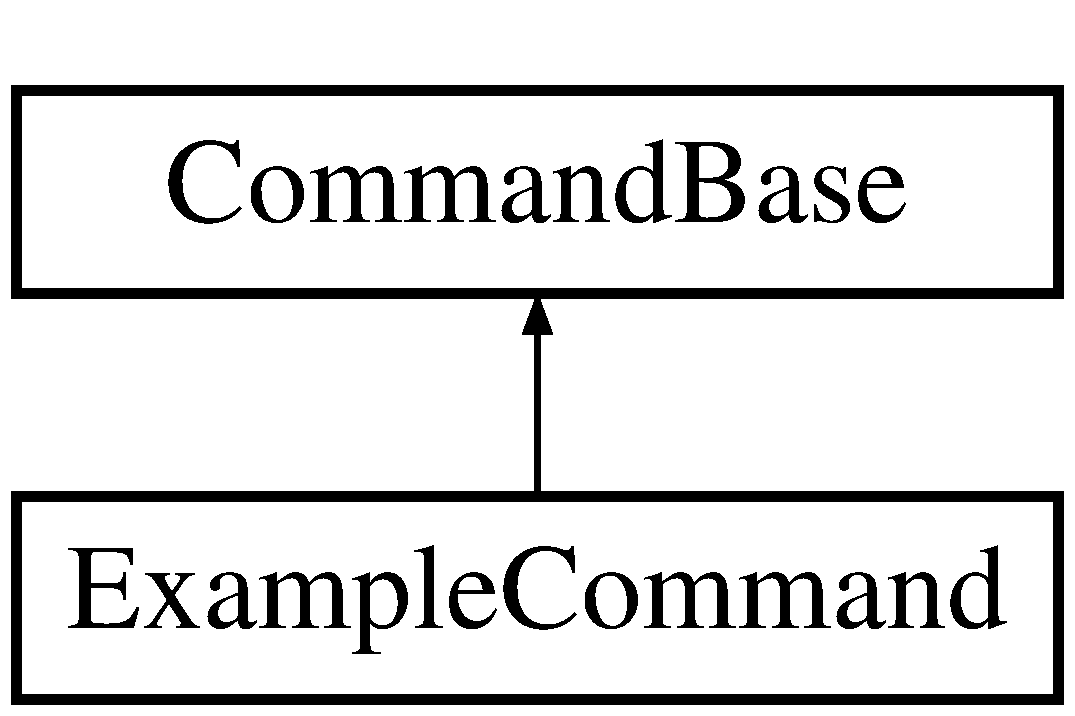
\includegraphics[height=2.000000cm]{class_command_base}
\end{center}
\end{figure}
\subsection*{\-Public \-Member \-Functions}
\begin{DoxyCompactItemize}
\item 
\hyperlink{class_command_base_a329ddd4c5a6ffd6c9d775a08c361823b}{\-Command\-Base} (const char $\ast$name)
\item 
\hyperlink{class_command_base_af42de9fe79dc64fce99580ee1e2f678f}{\-Command\-Base} ()
\end{DoxyCompactItemize}
\subsection*{\-Static \-Public \-Member \-Functions}
\begin{DoxyCompactItemize}
\item 
static void \hyperlink{class_command_base_a4dbfcd3b6ae92d752bc36a29dd1e1a5a}{init} ()
\end{DoxyCompactItemize}
\subsection*{\-Static \-Public \-Attributes}
\begin{DoxyCompactItemize}
\item 
static \hyperlink{class_drive}{\-Drive} $\ast$ \hyperlink{class_command_base_ad3e30f2241b0fc05c2dde2f20c1110c8}{s\-\_\-drive} = \-N\-U\-L\-L
\item 
static \hyperlink{class_ball_pickup}{\-Ball\-Pickup} $\ast$ \hyperlink{class_command_base_a06014394e7c262f1ef010dc2fe1b17a9}{s\-\_\-ball\-Pickup} = \-N\-U\-L\-L
\item 
static \hyperlink{class_ball_shooter}{\-Ball\-Shooter} $\ast$ \hyperlink{class_command_base_ac48c9220b0d3a09b0b058875eff8c650}{s\-\_\-ball\-Shooter} = \-N\-U\-L\-L
\item 
static \hyperlink{class_ball_storage}{\-Ball\-Storage} $\ast$ \hyperlink{class_command_base_a6e7f4b4c66e09b1d1d2e9496d0b018da}{s\-\_\-ball\-Storage} = \-N\-U\-L\-L
\item 
static \hyperlink{class_camera}{\-Camera} $\ast$ \hyperlink{class_command_base_a9586e8acac30698641eddb49066e1d47}{s\-\_\-camera} = \-N\-U\-L\-L
\item 
static \hyperlink{class_camera_mount}{\-Camera\-Mount} $\ast$ \hyperlink{class_command_base_a73790b416a401faa311259bd45f7aa47}{s\-\_\-camera\-Mount} = \-N\-U\-L\-L
\item 
static \hyperlink{class_gyro_subsystem}{\-Gyro\-Subsystem} $\ast$ \hyperlink{class_command_base_ab41fbac4795141797607460fedd04181}{s\-\_\-gyro} = \-N\-U\-L\-L
\item 
static \hyperlink{class_ultrasonic_sensor}{\-Ultrasonic\-Sensor} $\ast$ \hyperlink{class_command_base_a668786f77a2e65cd4f6beef52ba1538b}{s\-\_\-ultrasonic\-Sensor} = \-N\-U\-L\-L
\item 
static \hyperlink{class_accelerometer_subsystem}{\-Accelerometer\-Subsystem} $\ast$ \hyperlink{class_command_base_a2fd849df3b42d41c784179506228e841}{s\-\_\-accelerometer} = \-N\-U\-L\-L
\item 
static \hyperlink{class_o_i}{\-O\-I} $\ast$ \hyperlink{class_command_base_ae6807501159925367f8008fc0534eda5}{oi} = \-N\-U\-L\-L
\end{DoxyCompactItemize}


\subsection{\-Detailed \-Description}
\-The base for all commands. \-All atomic commands should subclass \hyperlink{class_command_base}{\-Command\-Base}. \hyperlink{class_command_base}{\-Command\-Base} stores creates and stores each control system. \-To access a subsystem elsewhere in your code in your code use \-Command\-Base.\-examplesubsystem. 

\begin{DoxyAuthor}{\-Author}
\-Arthur \-Lockman 
\end{DoxyAuthor}


\-Definition at line 24 of file \-Command\-Base.\-h.



\subsection{\-Constructor \& \-Destructor \-Documentation}
\hypertarget{class_command_base_a329ddd4c5a6ffd6c9d775a08c361823b}{\index{\-Command\-Base@{\-Command\-Base}!\-Command\-Base@{\-Command\-Base}}
\index{\-Command\-Base@{\-Command\-Base}!CommandBase@{\-Command\-Base}}
\subsubsection[{\-Command\-Base}]{\setlength{\rightskip}{0pt plus 5cm}{\bf \-Command\-Base\-::\-Command\-Base} (
\begin{DoxyParamCaption}
\item[{const char $\ast$}]{name}
\end{DoxyParamCaption}
)}}\label{class_command_base_a329ddd4c5a6ffd6c9d775a08c361823b}


\-Definition at line 4 of file \-Command\-Base.\-cpp.

\hypertarget{class_command_base_af42de9fe79dc64fce99580ee1e2f678f}{\index{\-Command\-Base@{\-Command\-Base}!\-Command\-Base@{\-Command\-Base}}
\index{\-Command\-Base@{\-Command\-Base}!CommandBase@{\-Command\-Base}}
\subsubsection[{\-Command\-Base}]{\setlength{\rightskip}{0pt plus 5cm}{\bf \-Command\-Base\-::\-Command\-Base} (
\begin{DoxyParamCaption}
{}
\end{DoxyParamCaption}
)}}\label{class_command_base_af42de9fe79dc64fce99580ee1e2f678f}


\-Definition at line 9 of file \-Command\-Base.\-cpp.



\subsection{\-Member \-Function \-Documentation}
\hypertarget{class_command_base_a4dbfcd3b6ae92d752bc36a29dd1e1a5a}{\index{\-Command\-Base@{\-Command\-Base}!init@{init}}
\index{init@{init}!CommandBase@{\-Command\-Base}}
\subsubsection[{init}]{\setlength{\rightskip}{0pt plus 5cm}void {\bf \-Command\-Base\-::init} (
\begin{DoxyParamCaption}
{}
\end{DoxyParamCaption}
)\hspace{0.3cm}{\ttfamily  \mbox{[}static\mbox{]}}}}\label{class_command_base_a4dbfcd3b6ae92d752bc36a29dd1e1a5a}


\-Definition at line 27 of file \-Command\-Base.\-cpp.



\subsection{\-Member \-Data \-Documentation}
\hypertarget{class_command_base_ae6807501159925367f8008fc0534eda5}{\index{\-Command\-Base@{\-Command\-Base}!oi@{oi}}
\index{oi@{oi}!CommandBase@{\-Command\-Base}}
\subsubsection[{oi}]{\setlength{\rightskip}{0pt plus 5cm}{\bf \-O\-I} $\ast$ {\bf \-Command\-Base\-::oi} = \-N\-U\-L\-L\hspace{0.3cm}{\ttfamily  \mbox{[}static\mbox{]}}}}\label{class_command_base_ae6807501159925367f8008fc0534eda5}


\-Definition at line 43 of file \-Command\-Base.\-h.

\hypertarget{class_command_base_a2fd849df3b42d41c784179506228e841}{\index{\-Command\-Base@{\-Command\-Base}!s\-\_\-accelerometer@{s\-\_\-accelerometer}}
\index{s\-\_\-accelerometer@{s\-\_\-accelerometer}!CommandBase@{\-Command\-Base}}
\subsubsection[{s\-\_\-accelerometer}]{\setlength{\rightskip}{0pt plus 5cm}{\bf \-Accelerometer\-Subsystem} $\ast$ {\bf \-Command\-Base\-::s\-\_\-accelerometer} = \-N\-U\-L\-L\hspace{0.3cm}{\ttfamily  \mbox{[}static\mbox{]}}}}\label{class_command_base_a2fd849df3b42d41c784179506228e841}


\-Definition at line 40 of file \-Command\-Base.\-h.

\hypertarget{class_command_base_a06014394e7c262f1ef010dc2fe1b17a9}{\index{\-Command\-Base@{\-Command\-Base}!s\-\_\-ball\-Pickup@{s\-\_\-ball\-Pickup}}
\index{s\-\_\-ball\-Pickup@{s\-\_\-ball\-Pickup}!CommandBase@{\-Command\-Base}}
\subsubsection[{s\-\_\-ball\-Pickup}]{\setlength{\rightskip}{0pt plus 5cm}{\bf \-Ball\-Pickup} $\ast$ {\bf \-Command\-Base\-::s\-\_\-ball\-Pickup} = \-N\-U\-L\-L\hspace{0.3cm}{\ttfamily  \mbox{[}static\mbox{]}}}}\label{class_command_base_a06014394e7c262f1ef010dc2fe1b17a9}


\-Definition at line 33 of file \-Command\-Base.\-h.

\hypertarget{class_command_base_ac48c9220b0d3a09b0b058875eff8c650}{\index{\-Command\-Base@{\-Command\-Base}!s\-\_\-ball\-Shooter@{s\-\_\-ball\-Shooter}}
\index{s\-\_\-ball\-Shooter@{s\-\_\-ball\-Shooter}!CommandBase@{\-Command\-Base}}
\subsubsection[{s\-\_\-ball\-Shooter}]{\setlength{\rightskip}{0pt plus 5cm}{\bf \-Ball\-Shooter} $\ast$ {\bf \-Command\-Base\-::s\-\_\-ball\-Shooter} = \-N\-U\-L\-L\hspace{0.3cm}{\ttfamily  \mbox{[}static\mbox{]}}}}\label{class_command_base_ac48c9220b0d3a09b0b058875eff8c650}


\-Definition at line 34 of file \-Command\-Base.\-h.

\hypertarget{class_command_base_a6e7f4b4c66e09b1d1d2e9496d0b018da}{\index{\-Command\-Base@{\-Command\-Base}!s\-\_\-ball\-Storage@{s\-\_\-ball\-Storage}}
\index{s\-\_\-ball\-Storage@{s\-\_\-ball\-Storage}!CommandBase@{\-Command\-Base}}
\subsubsection[{s\-\_\-ball\-Storage}]{\setlength{\rightskip}{0pt plus 5cm}{\bf \-Ball\-Storage} $\ast$ {\bf \-Command\-Base\-::s\-\_\-ball\-Storage} = \-N\-U\-L\-L\hspace{0.3cm}{\ttfamily  \mbox{[}static\mbox{]}}}}\label{class_command_base_a6e7f4b4c66e09b1d1d2e9496d0b018da}


\-Definition at line 35 of file \-Command\-Base.\-h.

\hypertarget{class_command_base_a9586e8acac30698641eddb49066e1d47}{\index{\-Command\-Base@{\-Command\-Base}!s\-\_\-camera@{s\-\_\-camera}}
\index{s\-\_\-camera@{s\-\_\-camera}!CommandBase@{\-Command\-Base}}
\subsubsection[{s\-\_\-camera}]{\setlength{\rightskip}{0pt plus 5cm}{\bf \-Camera} $\ast$ {\bf \-Command\-Base\-::s\-\_\-camera} = \-N\-U\-L\-L\hspace{0.3cm}{\ttfamily  \mbox{[}static\mbox{]}}}}\label{class_command_base_a9586e8acac30698641eddb49066e1d47}


\-Definition at line 36 of file \-Command\-Base.\-h.

\hypertarget{class_command_base_a73790b416a401faa311259bd45f7aa47}{\index{\-Command\-Base@{\-Command\-Base}!s\-\_\-camera\-Mount@{s\-\_\-camera\-Mount}}
\index{s\-\_\-camera\-Mount@{s\-\_\-camera\-Mount}!CommandBase@{\-Command\-Base}}
\subsubsection[{s\-\_\-camera\-Mount}]{\setlength{\rightskip}{0pt plus 5cm}{\bf \-Camera\-Mount} $\ast$ {\bf \-Command\-Base\-::s\-\_\-camera\-Mount} = \-N\-U\-L\-L\hspace{0.3cm}{\ttfamily  \mbox{[}static\mbox{]}}}}\label{class_command_base_a73790b416a401faa311259bd45f7aa47}


\-Definition at line 37 of file \-Command\-Base.\-h.

\hypertarget{class_command_base_ad3e30f2241b0fc05c2dde2f20c1110c8}{\index{\-Command\-Base@{\-Command\-Base}!s\-\_\-drive@{s\-\_\-drive}}
\index{s\-\_\-drive@{s\-\_\-drive}!CommandBase@{\-Command\-Base}}
\subsubsection[{s\-\_\-drive}]{\setlength{\rightskip}{0pt plus 5cm}{\bf \-Drive} $\ast$ {\bf \-Command\-Base\-::s\-\_\-drive} = \-N\-U\-L\-L\hspace{0.3cm}{\ttfamily  \mbox{[}static\mbox{]}}}}\label{class_command_base_ad3e30f2241b0fc05c2dde2f20c1110c8}


\-Definition at line 32 of file \-Command\-Base.\-h.

\hypertarget{class_command_base_ab41fbac4795141797607460fedd04181}{\index{\-Command\-Base@{\-Command\-Base}!s\-\_\-gyro@{s\-\_\-gyro}}
\index{s\-\_\-gyro@{s\-\_\-gyro}!CommandBase@{\-Command\-Base}}
\subsubsection[{s\-\_\-gyro}]{\setlength{\rightskip}{0pt plus 5cm}{\bf \-Gyro\-Subsystem} $\ast$ {\bf \-Command\-Base\-::s\-\_\-gyro} = \-N\-U\-L\-L\hspace{0.3cm}{\ttfamily  \mbox{[}static\mbox{]}}}}\label{class_command_base_ab41fbac4795141797607460fedd04181}


\-Definition at line 38 of file \-Command\-Base.\-h.

\hypertarget{class_command_base_a668786f77a2e65cd4f6beef52ba1538b}{\index{\-Command\-Base@{\-Command\-Base}!s\-\_\-ultrasonic\-Sensor@{s\-\_\-ultrasonic\-Sensor}}
\index{s\-\_\-ultrasonic\-Sensor@{s\-\_\-ultrasonic\-Sensor}!CommandBase@{\-Command\-Base}}
\subsubsection[{s\-\_\-ultrasonic\-Sensor}]{\setlength{\rightskip}{0pt plus 5cm}{\bf \-Ultrasonic\-Sensor} $\ast$ {\bf \-Command\-Base\-::s\-\_\-ultrasonic\-Sensor} = \-N\-U\-L\-L\hspace{0.3cm}{\ttfamily  \mbox{[}static\mbox{]}}}}\label{class_command_base_a668786f77a2e65cd4f6beef52ba1538b}


\-Definition at line 39 of file \-Command\-Base.\-h.



\-The documentation for this class was generated from the following files\-:\begin{DoxyCompactItemize}
\item 
\-Y\-:/\-Rebound\-Rumble-\/\-Trunk/\-Project/\hyperlink{_command_base_8h}{\-Command\-Base.\-h}\item 
\-Y\-:/\-Rebound\-Rumble-\/\-Trunk/\-Project/\hyperlink{_command_base_8cpp}{\-Command\-Base.\-cpp}\end{DoxyCompactItemize}

\hypertarget{class_drive}{\section{\-Drive \-Class \-Reference}
\label{class_drive}\index{\-Drive@{\-Drive}}
}


\-The drive object for the robot. \-All methods for interacting with drive will go here.  




{\ttfamily \#include $<$\-Drive.\-h$>$}

\subsection*{\-Public \-Member \-Functions}
\begin{DoxyCompactItemize}
\item 
\hyperlink{class_drive_af18ec3b1c1c6603185fd4f2c9d5d6ac6}{\-Drive} ()
\item 
void \hyperlink{class_drive_abd6c9c8a666e4faaa47fc84a3e0a33bf}{\-Init\-Default\-Command} ()
\end{DoxyCompactItemize}


\subsection{\-Detailed \-Description}
\-The drive object for the robot. \-All methods for interacting with drive will go here. 

\begin{DoxyAuthor}{\-Author}
\-Arthur \-Lockman 
\end{DoxyAuthor}


\-Definition at line 13 of file \-Drive.\-h.



\subsection{\-Constructor \& \-Destructor \-Documentation}
\hypertarget{class_drive_af18ec3b1c1c6603185fd4f2c9d5d6ac6}{\index{\-Drive@{\-Drive}!\-Drive@{\-Drive}}
\index{\-Drive@{\-Drive}!Drive@{\-Drive}}
\subsubsection[{\-Drive}]{\setlength{\rightskip}{0pt plus 5cm}{\bf \-Drive\-::\-Drive} (
\begin{DoxyParamCaption}
{}
\end{DoxyParamCaption}
)}}\label{class_drive_af18ec3b1c1c6603185fd4f2c9d5d6ac6}


\-Definition at line 4 of file \-Drive.\-cpp.



\subsection{\-Member \-Function \-Documentation}
\hypertarget{class_drive_abd6c9c8a666e4faaa47fc84a3e0a33bf}{\index{\-Drive@{\-Drive}!\-Init\-Default\-Command@{\-Init\-Default\-Command}}
\index{\-Init\-Default\-Command@{\-Init\-Default\-Command}!Drive@{\-Drive}}
\subsubsection[{\-Init\-Default\-Command}]{\setlength{\rightskip}{0pt plus 5cm}void {\bf \-Drive\-::\-Init\-Default\-Command} (
\begin{DoxyParamCaption}
{}
\end{DoxyParamCaption}
)}}\label{class_drive_abd6c9c8a666e4faaa47fc84a3e0a33bf}


\-Definition at line 9 of file \-Drive.\-cpp.



\-The documentation for this class was generated from the following files\-:\begin{DoxyCompactItemize}
\item 
\-Y\-:/\-Rebound\-Rumble-\/\-Trunk/\-Project/\-Subsystems/\hyperlink{_drive_8h}{\-Drive.\-h}\item 
\-Y\-:/\-Rebound\-Rumble-\/\-Trunk/\-Project/\-Subsystems/\hyperlink{_drive_8cpp}{\-Drive.\-cpp}\end{DoxyCompactItemize}

\hypertarget{class_example_command}{\section{\-Example\-Command \-Class \-Reference}
\label{class_example_command}\index{\-Example\-Command@{\-Example\-Command}}
}


{\ttfamily \#include $<$\-Example\-Command.\-h$>$}

\-Inheritance diagram for \-Example\-Command\-:\begin{figure}[H]
\begin{center}
\leavevmode
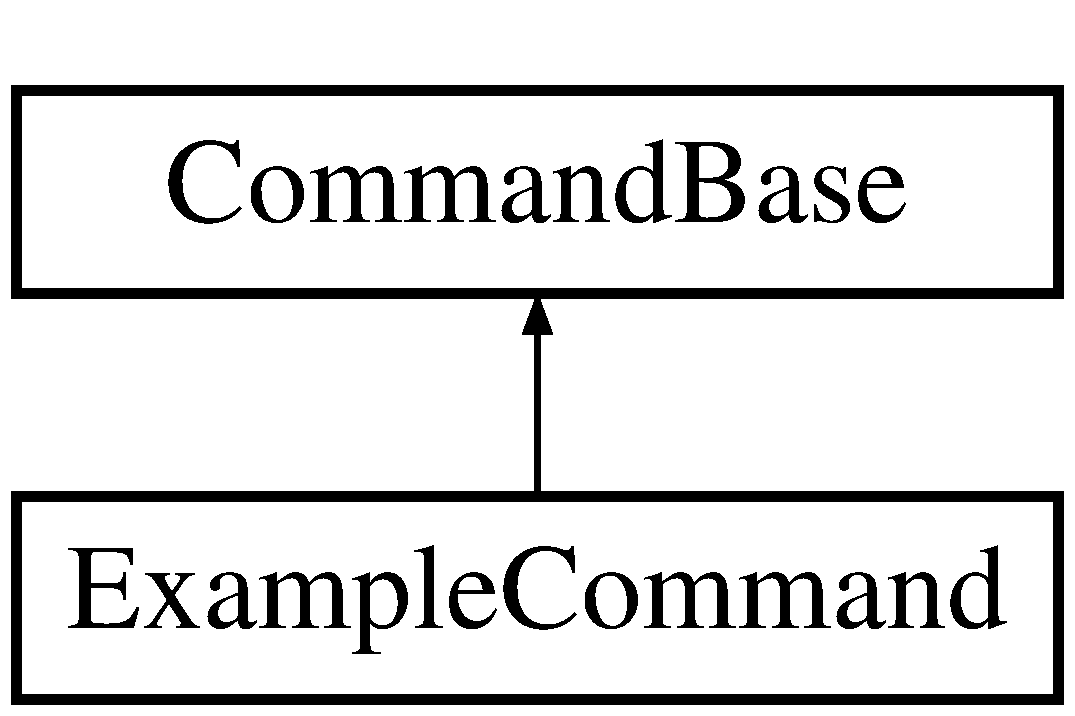
\includegraphics[height=2.000000cm]{class_example_command}
\end{center}
\end{figure}
\subsection*{\-Public \-Member \-Functions}
\begin{DoxyCompactItemize}
\item 
\hyperlink{class_example_command_ad91449e429d7da554dd5d984a0874a24}{\-Example\-Command} ()
\item 
virtual void \hyperlink{class_example_command_a212ebaa8787be1d969df8baad33e773e}{\-Initialize} ()
\item 
virtual void \hyperlink{class_example_command_a660f54d7a94499d134eda80c0247a86d}{\-Execute} ()
\item 
virtual bool \hyperlink{class_example_command_a3fb5743096b8ecf222dac4217df29f3f}{\-Is\-Finished} ()
\item 
virtual void \hyperlink{class_example_command_a462af4143f6a5d62ffcfa7c1bb2d045f}{\-End} ()
\item 
virtual void \hyperlink{class_example_command_a3a7220e2adf254aa788a837e38064c9e}{\-Interrupted} ()
\end{DoxyCompactItemize}


\subsection{\-Detailed \-Description}
\begin{DoxyAuthor}{\-Author}
\-Example\-Author 
\end{DoxyAuthor}


\-Definition at line 11 of file \-Example\-Command.\-h.



\subsection{\-Constructor \& \-Destructor \-Documentation}
\hypertarget{class_example_command_ad91449e429d7da554dd5d984a0874a24}{\index{\-Example\-Command@{\-Example\-Command}!\-Example\-Command@{\-Example\-Command}}
\index{\-Example\-Command@{\-Example\-Command}!ExampleCommand@{\-Example\-Command}}
\subsubsection[{\-Example\-Command}]{\setlength{\rightskip}{0pt plus 5cm}{\bf \-Example\-Command\-::\-Example\-Command} (
\begin{DoxyParamCaption}
{}
\end{DoxyParamCaption}
)}}\label{class_example_command_ad91449e429d7da554dd5d984a0874a24}


\-Definition at line 3 of file \-Example\-Command.\-cpp.



\subsection{\-Member \-Function \-Documentation}
\hypertarget{class_example_command_a462af4143f6a5d62ffcfa7c1bb2d045f}{\index{\-Example\-Command@{\-Example\-Command}!\-End@{\-End}}
\index{\-End@{\-End}!ExampleCommand@{\-Example\-Command}}
\subsubsection[{\-End}]{\setlength{\rightskip}{0pt plus 5cm}void {\bf \-Example\-Command\-::\-End} (
\begin{DoxyParamCaption}
{}
\end{DoxyParamCaption}
)\hspace{0.3cm}{\ttfamily  \mbox{[}virtual\mbox{]}}}}\label{class_example_command_a462af4143f6a5d62ffcfa7c1bb2d045f}


\-Definition at line 24 of file \-Example\-Command.\-cpp.

\hypertarget{class_example_command_a660f54d7a94499d134eda80c0247a86d}{\index{\-Example\-Command@{\-Example\-Command}!\-Execute@{\-Execute}}
\index{\-Execute@{\-Execute}!ExampleCommand@{\-Example\-Command}}
\subsubsection[{\-Execute}]{\setlength{\rightskip}{0pt plus 5cm}void {\bf \-Example\-Command\-::\-Execute} (
\begin{DoxyParamCaption}
{}
\end{DoxyParamCaption}
)\hspace{0.3cm}{\ttfamily  \mbox{[}virtual\mbox{]}}}}\label{class_example_command_a660f54d7a94499d134eda80c0247a86d}


\-Definition at line 14 of file \-Example\-Command.\-cpp.

\hypertarget{class_example_command_a212ebaa8787be1d969df8baad33e773e}{\index{\-Example\-Command@{\-Example\-Command}!\-Initialize@{\-Initialize}}
\index{\-Initialize@{\-Initialize}!ExampleCommand@{\-Example\-Command}}
\subsubsection[{\-Initialize}]{\setlength{\rightskip}{0pt plus 5cm}void {\bf \-Example\-Command\-::\-Initialize} (
\begin{DoxyParamCaption}
{}
\end{DoxyParamCaption}
)\hspace{0.3cm}{\ttfamily  \mbox{[}virtual\mbox{]}}}}\label{class_example_command_a212ebaa8787be1d969df8baad33e773e}


\-Definition at line 9 of file \-Example\-Command.\-cpp.

\hypertarget{class_example_command_a3a7220e2adf254aa788a837e38064c9e}{\index{\-Example\-Command@{\-Example\-Command}!\-Interrupted@{\-Interrupted}}
\index{\-Interrupted@{\-Interrupted}!ExampleCommand@{\-Example\-Command}}
\subsubsection[{\-Interrupted}]{\setlength{\rightskip}{0pt plus 5cm}void {\bf \-Example\-Command\-::\-Interrupted} (
\begin{DoxyParamCaption}
{}
\end{DoxyParamCaption}
)\hspace{0.3cm}{\ttfamily  \mbox{[}virtual\mbox{]}}}}\label{class_example_command_a3a7220e2adf254aa788a837e38064c9e}


\-Definition at line 30 of file \-Example\-Command.\-cpp.

\hypertarget{class_example_command_a3fb5743096b8ecf222dac4217df29f3f}{\index{\-Example\-Command@{\-Example\-Command}!\-Is\-Finished@{\-Is\-Finished}}
\index{\-Is\-Finished@{\-Is\-Finished}!ExampleCommand@{\-Example\-Command}}
\subsubsection[{\-Is\-Finished}]{\setlength{\rightskip}{0pt plus 5cm}bool {\bf \-Example\-Command\-::\-Is\-Finished} (
\begin{DoxyParamCaption}
{}
\end{DoxyParamCaption}
)\hspace{0.3cm}{\ttfamily  \mbox{[}virtual\mbox{]}}}}\label{class_example_command_a3fb5743096b8ecf222dac4217df29f3f}


\-Definition at line 19 of file \-Example\-Command.\-cpp.



\-The documentation for this class was generated from the following files\-:\begin{DoxyCompactItemize}
\item 
\-Y\-:/\-Rebound\-Rumble-\/\-Trunk/\-Project/\-Commands/\hyperlink{_example_command_8h}{\-Example\-Command.\-h}\item 
\-Y\-:/\-Rebound\-Rumble-\/\-Trunk/\-Project/\-Commands/\hyperlink{_example_command_8cpp}{\-Example\-Command.\-cpp}\end{DoxyCompactItemize}

\hypertarget{class_gyro_subsystem}{\section{\-Gyro\-Subsystem \-Class \-Reference}
\label{class_gyro_subsystem}\index{\-Gyro\-Subsystem@{\-Gyro\-Subsystem}}
}


\-This controls the gyro sensor that will go onto the robot. \-All methods for interacting with the gyro go here.  




{\ttfamily \#include $<$\-Gyro\-Subsystem.\-h$>$}

\subsection*{\-Public \-Member \-Functions}
\begin{DoxyCompactItemize}
\item 
\hyperlink{class_gyro_subsystem_ac60bb063901c17dd9f827fafc5f52011}{\-Gyro\-Subsystem} ()
\item 
void \hyperlink{class_gyro_subsystem_a4f80be505ad1347cfddb52903d347569}{\-Init\-Default\-Command} ()
\end{DoxyCompactItemize}


\subsection{\-Detailed \-Description}
\-This controls the gyro sensor that will go onto the robot. \-All methods for interacting with the gyro go here. 

\begin{DoxyAuthor}{\-Author}
\-Arthur \-Lockman 
\end{DoxyAuthor}


\-Definition at line 13 of file \-Gyro\-Subsystem.\-h.



\subsection{\-Constructor \& \-Destructor \-Documentation}
\hypertarget{class_gyro_subsystem_ac60bb063901c17dd9f827fafc5f52011}{\index{\-Gyro\-Subsystem@{\-Gyro\-Subsystem}!\-Gyro\-Subsystem@{\-Gyro\-Subsystem}}
\index{\-Gyro\-Subsystem@{\-Gyro\-Subsystem}!GyroSubsystem@{\-Gyro\-Subsystem}}
\subsubsection[{\-Gyro\-Subsystem}]{\setlength{\rightskip}{0pt plus 5cm}{\bf \-Gyro\-Subsystem\-::\-Gyro\-Subsystem} (
\begin{DoxyParamCaption}
{}
\end{DoxyParamCaption}
)}}\label{class_gyro_subsystem_ac60bb063901c17dd9f827fafc5f52011}


\-Definition at line 4 of file \-Gyro\-Subsystem.\-cpp.



\subsection{\-Member \-Function \-Documentation}
\hypertarget{class_gyro_subsystem_a4f80be505ad1347cfddb52903d347569}{\index{\-Gyro\-Subsystem@{\-Gyro\-Subsystem}!\-Init\-Default\-Command@{\-Init\-Default\-Command}}
\index{\-Init\-Default\-Command@{\-Init\-Default\-Command}!GyroSubsystem@{\-Gyro\-Subsystem}}
\subsubsection[{\-Init\-Default\-Command}]{\setlength{\rightskip}{0pt plus 5cm}void {\bf \-Gyro\-Subsystem\-::\-Init\-Default\-Command} (
\begin{DoxyParamCaption}
{}
\end{DoxyParamCaption}
)}}\label{class_gyro_subsystem_a4f80be505ad1347cfddb52903d347569}


\-Definition at line 8 of file \-Gyro\-Subsystem.\-cpp.



\-The documentation for this class was generated from the following files\-:\begin{DoxyCompactItemize}
\item 
\-Y\-:/\-Rebound\-Rumble-\/\-Trunk/\-Project/\-Subsystems/\hyperlink{_gyro_subsystem_8h}{\-Gyro\-Subsystem.\-h}\item 
\-Y\-:/\-Rebound\-Rumble-\/\-Trunk/\-Project/\-Subsystems/\hyperlink{_gyro_subsystem_8cpp}{\-Gyro\-Subsystem.\-cpp}\end{DoxyCompactItemize}

\hypertarget{class_o_i}{\section{\-O\-I \-Class \-Reference}
\label{class_o_i}\index{\-O\-I@{\-O\-I}}
}


\-All of the classes for interacting with the operator interface go here.  




{\ttfamily \#include $<$\-O\-I.\-h$>$}

\subsection*{\-Public \-Member \-Functions}
\begin{DoxyCompactItemize}
\item 
\hyperlink{class_o_i_a77c2c4630ca19e64a7885154f3dc202f}{\-O\-I} ()
\begin{DoxyCompactList}\small\item\em \-Constructs all of the \-Operator \-Interface classes for interacting with the robot. \end{DoxyCompactList}\end{DoxyCompactItemize}
\subsection*{\-Public \-Attributes}
\begin{DoxyCompactItemize}
\item 
\hyperlink{class_xbox_joystick}{\-Xbox\-Joystick} \hyperlink{class_o_i_a7d11d42696e135b067edd10f24597326}{stick}
\end{DoxyCompactItemize}


\subsection{\-Detailed \-Description}
\-All of the classes for interacting with the operator interface go here. 

\begin{DoxyAuthor}{\-Author}
\-Arthur \-Lockman 
\end{DoxyAuthor}


\-Definition at line 13 of file \-O\-I.\-h.



\subsection{\-Constructor \& \-Destructor \-Documentation}
\hypertarget{class_o_i_a77c2c4630ca19e64a7885154f3dc202f}{\index{\-O\-I@{\-O\-I}!\-O\-I@{\-O\-I}}
\index{\-O\-I@{\-O\-I}!OI@{\-O\-I}}
\subsubsection[{\-O\-I}]{\setlength{\rightskip}{0pt plus 5cm}{\bf \-O\-I\-::\-O\-I} (
\begin{DoxyParamCaption}
{}
\end{DoxyParamCaption}
)}}\label{class_o_i_a77c2c4630ca19e64a7885154f3dc202f}


\-Constructs all of the \-Operator \-Interface classes for interacting with the robot. 



\-Definition at line 8 of file \-O\-I.\-cpp.



\subsection{\-Member \-Data \-Documentation}
\hypertarget{class_o_i_a7d11d42696e135b067edd10f24597326}{\index{\-O\-I@{\-O\-I}!stick@{stick}}
\index{stick@{stick}!OI@{\-O\-I}}
\subsubsection[{stick}]{\setlength{\rightskip}{0pt plus 5cm}{\bf \-Xbox\-Joystick} {\bf \-O\-I\-::stick}}}\label{class_o_i_a7d11d42696e135b067edd10f24597326}


\-Definition at line 19 of file \-O\-I.\-h.



\-The documentation for this class was generated from the following files\-:\begin{DoxyCompactItemize}
\item 
\-Y\-:/\-Rebound\-Rumble-\/\-Trunk/\-Project/\hyperlink{_o_i_8h}{\-O\-I.\-h}\item 
\-Y\-:/\-Rebound\-Rumble-\/\-Trunk/\-Project/\hyperlink{_o_i_8cpp}{\-O\-I.\-cpp}\end{DoxyCompactItemize}

\hypertarget{class_rebound_rumble_bot}{\section{\-Rebound\-Rumble\-Bot \-Class \-Reference}
\label{class_rebound_rumble_bot}\index{\-Rebound\-Rumble\-Bot@{\-Rebound\-Rumble\-Bot}}
}


\-This class controls the entire robot, everything it does, and all of its interactions with the field, itself, and the operators.  




\subsection{\-Detailed \-Description}
\-This class controls the entire robot, everything it does, and all of its interactions with the field, itself, and the operators. 

\begin{DoxyAuthor}{\-Author}
\-Arthur \-Lockman 
\end{DoxyAuthor}


\-Definition at line 13 of file \-Rebound\-Rumble\-Bot.\-cpp.



\-The documentation for this class was generated from the following file\-:\begin{DoxyCompactItemize}
\item 
\-Y\-:/\-Rebound\-Rumble-\/\-Trunk/\-Project/\hyperlink{_rebound_rumble_bot_8cpp}{\-Rebound\-Rumble\-Bot.\-cpp}\end{DoxyCompactItemize}

\hypertarget{class_ultrasonic_sensor}{\section{\-Ultrasonic\-Sensor \-Class \-Reference}
\label{class_ultrasonic_sensor}\index{\-Ultrasonic\-Sensor@{\-Ultrasonic\-Sensor}}
}


\-This class controls the \-Ultrasonic \-Range \-Finding \-Sensor on the robot. \-All methods for interacting with that sensor will go here.  




{\ttfamily \#include $<$\-Ultrasonic\-Sensor.\-h$>$}

\subsection*{\-Public \-Member \-Functions}
\begin{DoxyCompactItemize}
\item 
\hyperlink{class_ultrasonic_sensor_afc21cb39ba75dfd008e1e82c82d2e61f}{\-Ultrasonic\-Sensor} ()
\item 
void \hyperlink{class_ultrasonic_sensor_a35b733517f59700a03dc26f154bc5da2}{\-Init\-Default\-Command} ()
\end{DoxyCompactItemize}


\subsection{\-Detailed \-Description}
\-This class controls the \-Ultrasonic \-Range \-Finding \-Sensor on the robot. \-All methods for interacting with that sensor will go here. 

\begin{DoxyAuthor}{\-Author}
\-Arthur \-Lockman 
\end{DoxyAuthor}


\-Definition at line 13 of file \-Ultrasonic\-Sensor.\-h.



\subsection{\-Constructor \& \-Destructor \-Documentation}
\hypertarget{class_ultrasonic_sensor_afc21cb39ba75dfd008e1e82c82d2e61f}{\index{\-Ultrasonic\-Sensor@{\-Ultrasonic\-Sensor}!\-Ultrasonic\-Sensor@{\-Ultrasonic\-Sensor}}
\index{\-Ultrasonic\-Sensor@{\-Ultrasonic\-Sensor}!UltrasonicSensor@{\-Ultrasonic\-Sensor}}
\subsubsection[{\-Ultrasonic\-Sensor}]{\setlength{\rightskip}{0pt plus 5cm}{\bf \-Ultrasonic\-Sensor\-::\-Ultrasonic\-Sensor} (
\begin{DoxyParamCaption}
{}
\end{DoxyParamCaption}
)}}\label{class_ultrasonic_sensor_afc21cb39ba75dfd008e1e82c82d2e61f}


\-Definition at line 4 of file \-Ultrasonic\-Sensor.\-cpp.



\subsection{\-Member \-Function \-Documentation}
\hypertarget{class_ultrasonic_sensor_a35b733517f59700a03dc26f154bc5da2}{\index{\-Ultrasonic\-Sensor@{\-Ultrasonic\-Sensor}!\-Init\-Default\-Command@{\-Init\-Default\-Command}}
\index{\-Init\-Default\-Command@{\-Init\-Default\-Command}!UltrasonicSensor@{\-Ultrasonic\-Sensor}}
\subsubsection[{\-Init\-Default\-Command}]{\setlength{\rightskip}{0pt plus 5cm}void {\bf \-Ultrasonic\-Sensor\-::\-Init\-Default\-Command} (
\begin{DoxyParamCaption}
{}
\end{DoxyParamCaption}
)}}\label{class_ultrasonic_sensor_a35b733517f59700a03dc26f154bc5da2}


\-Definition at line 8 of file \-Ultrasonic\-Sensor.\-cpp.



\-The documentation for this class was generated from the following files\-:\begin{DoxyCompactItemize}
\item 
\-Y\-:/\-Rebound\-Rumble-\/\-Trunk/\-Project/\-Subsystems/\hyperlink{_ultrasonic_sensor_8h}{\-Ultrasonic\-Sensor.\-h}\item 
\-Y\-:/\-Rebound\-Rumble-\/\-Trunk/\-Project/\-Subsystems/\hyperlink{_ultrasonic_sensor_8cpp}{\-Ultrasonic\-Sensor.\-cpp}\end{DoxyCompactItemize}

\hypertarget{class_xbox_joystick}{\section{\-Xbox\-Joystick \-Class \-Reference}
\label{class_xbox_joystick}\index{\-Xbox\-Joystick@{\-Xbox\-Joystick}}
}


{\ttfamily \#include $<$\-Xbox\-Joystick.\-h$>$}

\subsection*{\-Public \-Member \-Functions}
\begin{DoxyCompactItemize}
\item 
\hyperlink{class_xbox_joystick_a8592bd46942d57e14bd017eef9043159}{\-Xbox\-Joystick} ()
\begin{DoxyCompactList}\small\item\em \-This class constructs the instance of the \-X\-Box \-Joystick. \-It automatically calculates the deadband for the joysticks on the controller. \end{DoxyCompactList}\item 
float \hyperlink{class_xbox_joystick_a4192c8735c467d34c55074522fd3eeb1}{\-Get\-X} (\-Joystick\-Hand)
\begin{DoxyCompactList}\small\item\em \-Gets the value from the \-X axis of one of the joysticks on the controller. \end{DoxyCompactList}\item 
float \hyperlink{class_xbox_joystick_ab9f3fda49ebdf9fdec67b28726d3b910}{\-Get\-Y} (\-Joystick\-Hand)
\begin{DoxyCompactList}\small\item\em \-Gets the value from the \-Y axis of one of the joysticks on the controller. \end{DoxyCompactList}\item 
float \hyperlink{class_xbox_joystick_ad3c40b7a658f9d76615c82b96ab33bd9}{\-Get\-Magnitude} ()
\begin{DoxyCompactList}\small\item\em \-Gets the magnitude of the \-Y axis left joystick on the controller, which is used to find the speed that the robot should be moving at. \end{DoxyCompactList}\item 
float \hyperlink{class_xbox_joystick_a4924f582087f3e3aa1ab59103c427bb8}{\-Get\-Rotation} ()
\begin{DoxyCompactList}\small\item\em \-Gets the magnitude of the \-X axis right joystick on the controller, which is used to find the rotational direction that the robot should be moving in. \end{DoxyCompactList}\end{DoxyCompactItemize}


\subsection{\-Detailed \-Description}


\-Definition at line 15 of file \-Xbox\-Joystick.\-h.



\subsection{\-Constructor \& \-Destructor \-Documentation}
\hypertarget{class_xbox_joystick_a8592bd46942d57e14bd017eef9043159}{\index{\-Xbox\-Joystick@{\-Xbox\-Joystick}!\-Xbox\-Joystick@{\-Xbox\-Joystick}}
\index{\-Xbox\-Joystick@{\-Xbox\-Joystick}!XboxJoystick@{\-Xbox\-Joystick}}
\subsubsection[{\-Xbox\-Joystick}]{\setlength{\rightskip}{0pt plus 5cm}{\bf \-Xbox\-Joystick\-::\-Xbox\-Joystick} (
\begin{DoxyParamCaption}
{}
\end{DoxyParamCaption}
)}}\label{class_xbox_joystick_a8592bd46942d57e14bd017eef9043159}


\-This class constructs the instance of the \-X\-Box \-Joystick. \-It automatically calculates the deadband for the joysticks on the controller. 

\begin{DoxyAuthor}{\-Author}
\-Arthur \-Lockman 
\end{DoxyAuthor}


\-Definition at line 20 of file \-Xbox\-Joystick.\-cpp.



\subsection{\-Member \-Function \-Documentation}
\hypertarget{class_xbox_joystick_ad3c40b7a658f9d76615c82b96ab33bd9}{\index{\-Xbox\-Joystick@{\-Xbox\-Joystick}!\-Get\-Magnitude@{\-Get\-Magnitude}}
\index{\-Get\-Magnitude@{\-Get\-Magnitude}!XboxJoystick@{\-Xbox\-Joystick}}
\subsubsection[{\-Get\-Magnitude}]{\setlength{\rightskip}{0pt plus 5cm}float {\bf \-Xbox\-Joystick\-::\-Get\-Magnitude} (
\begin{DoxyParamCaption}
{}
\end{DoxyParamCaption}
)}}\label{class_xbox_joystick_ad3c40b7a658f9d76615c82b96ab33bd9}


\-Gets the magnitude of the \-Y axis left joystick on the controller, which is used to find the speed that the robot should be moving at. 

\begin{DoxyReturn}{\-Returns}
\-A float, positive is forward, and negative is backwards.
\end{DoxyReturn}
\begin{DoxyAuthor}{\-Author}
\-Arthur \-Lockman 
\end{DoxyAuthor}


\-Definition at line 71 of file \-Xbox\-Joystick.\-cpp.

\hypertarget{class_xbox_joystick_a4924f582087f3e3aa1ab59103c427bb8}{\index{\-Xbox\-Joystick@{\-Xbox\-Joystick}!\-Get\-Rotation@{\-Get\-Rotation}}
\index{\-Get\-Rotation@{\-Get\-Rotation}!XboxJoystick@{\-Xbox\-Joystick}}
\subsubsection[{\-Get\-Rotation}]{\setlength{\rightskip}{0pt plus 5cm}float {\bf \-Xbox\-Joystick\-::\-Get\-Rotation} (
\begin{DoxyParamCaption}
{}
\end{DoxyParamCaption}
)}}\label{class_xbox_joystick_a4924f582087f3e3aa1ab59103c427bb8}


\-Gets the magnitude of the \-X axis right joystick on the controller, which is used to find the rotational direction that the robot should be moving in. 

\begin{DoxyReturn}{\-Returns}
\-A float, positive is right, and negative is left.
\end{DoxyReturn}
\begin{DoxyAuthor}{\-Author}
\-Arthur \-Lockman 
\end{DoxyAuthor}


\-Definition at line 87 of file \-Xbox\-Joystick.\-cpp.

\hypertarget{class_xbox_joystick_a4192c8735c467d34c55074522fd3eeb1}{\index{\-Xbox\-Joystick@{\-Xbox\-Joystick}!\-Get\-X@{\-Get\-X}}
\index{\-Get\-X@{\-Get\-X}!XboxJoystick@{\-Xbox\-Joystick}}
\subsubsection[{\-Get\-X}]{\setlength{\rightskip}{0pt plus 5cm}float {\bf \-Xbox\-Joystick\-::\-Get\-X} (
\begin{DoxyParamCaption}
\item[{\-Joystick\-Hand}]{hand}
\end{DoxyParamCaption}
)}}\label{class_xbox_joystick_a4192c8735c467d34c55074522fd3eeb1}


\-Gets the value from the \-X axis of one of the joysticks on the controller. 


\begin{DoxyParams}{\-Parameters}
{\em hand} & \-The joystick hand to get, k\-Left\-Hand or k\-Right\-Hand.\\
\hline
\end{DoxyParams}
\begin{DoxyReturn}{\-Returns}
\-A float of the value of the \-X axis of the joystick.
\end{DoxyReturn}
\begin{DoxyAuthor}{\-Author}
\-Joseph \-Martin 
\end{DoxyAuthor}


\-Definition at line 38 of file \-Xbox\-Joystick.\-cpp.

\hypertarget{class_xbox_joystick_ab9f3fda49ebdf9fdec67b28726d3b910}{\index{\-Xbox\-Joystick@{\-Xbox\-Joystick}!\-Get\-Y@{\-Get\-Y}}
\index{\-Get\-Y@{\-Get\-Y}!XboxJoystick@{\-Xbox\-Joystick}}
\subsubsection[{\-Get\-Y}]{\setlength{\rightskip}{0pt plus 5cm}float {\bf \-Xbox\-Joystick\-::\-Get\-Y} (
\begin{DoxyParamCaption}
\item[{\-Joystick\-Hand}]{hand}
\end{DoxyParamCaption}
)}}\label{class_xbox_joystick_ab9f3fda49ebdf9fdec67b28726d3b910}


\-Gets the value from the \-Y axis of one of the joysticks on the controller. 


\begin{DoxyParams}{\-Parameters}
{\em hand} & \-The joystick hand to get, k\-Left\-Hand or k\-Right\-Hand.\\
\hline
\end{DoxyParams}
\begin{DoxyReturn}{\-Returns}
\-A float of the value of the \-Y axis of the joystick.
\end{DoxyReturn}
\begin{DoxyAuthor}{\-Author}
\-Joseph \-Martin 
\end{DoxyAuthor}


\-Definition at line 55 of file \-Xbox\-Joystick.\-cpp.



\-The documentation for this class was generated from the following files\-:\begin{DoxyCompactItemize}
\item 
\-Y\-:/\-Rebound\-Rumble-\/\-Trunk/\-Project/\-Classes/\hyperlink{_xbox_joystick_8h}{\-Xbox\-Joystick.\-h}\item 
\-Y\-:/\-Rebound\-Rumble-\/\-Trunk/\-Project/\-Classes/\hyperlink{_xbox_joystick_8cpp}{\-Xbox\-Joystick.\-cpp}\end{DoxyCompactItemize}

\chapter{\-File \-Documentation}
\hypertarget{_xbox_joystick_8cpp}{\section{\-Y\-:/\-Rebound\-Rumble-\/\-Trunk/\-Project/\-Classes/\-Xbox\-Joystick.cpp \-File \-Reference}
\label{_xbox_joystick_8cpp}\index{\-Y\-:/\-Rebound\-Rumble-\/\-Trunk/\-Project/\-Classes/\-Xbox\-Joystick.\-cpp@{\-Y\-:/\-Rebound\-Rumble-\/\-Trunk/\-Project/\-Classes/\-Xbox\-Joystick.\-cpp}}
}
{\ttfamily \#include \char`\"{}\-Xbox\-Joystick.\-h\char`\"{}}\*
{\ttfamily \#include \char`\"{}\-Joystick.\-h\char`\"{}}\*

\hypertarget{_xbox_joystick_8h}{\section{\-Y\-:/\-Rebound\-Rumble-\/\-Trunk/\-Project/\-Classes/\-Xbox\-Joystick.h \-File \-Reference}
\label{_xbox_joystick_8h}\index{\-Y\-:/\-Rebound\-Rumble-\/\-Trunk/\-Project/\-Classes/\-Xbox\-Joystick.\-h@{\-Y\-:/\-Rebound\-Rumble-\/\-Trunk/\-Project/\-Classes/\-Xbox\-Joystick.\-h}}
}
{\ttfamily \#include \char`\"{}\-W\-P\-I\-Lib.\-h\char`\"{}}\*
{\ttfamily \#include \char`\"{}../\-Robotmap.\-h\char`\"{}}\*
\subsection*{\-Classes}
\begin{DoxyCompactItemize}
\item 
class \hyperlink{class_xbox_joystick}{\-Xbox\-Joystick}
\end{DoxyCompactItemize}

\hypertarget{_command_base_8cpp}{\section{\-Y\-:/\-Rebound\-Rumble-\/\-Trunk/\-Project/\-Command\-Base.cpp \-File \-Reference}
\label{_command_base_8cpp}\index{\-Y\-:/\-Rebound\-Rumble-\/\-Trunk/\-Project/\-Command\-Base.\-cpp@{\-Y\-:/\-Rebound\-Rumble-\/\-Trunk/\-Project/\-Command\-Base.\-cpp}}
}
{\ttfamily \#include \char`\"{}\-Command\-Base.\-h\char`\"{}}\*
{\ttfamily \#include \char`\"{}\-Commands/\-Scheduler.\-h\char`\"{}}\*

\hypertarget{_command_base_8h}{\section{\-Y\-:/\-Rebound\-Rumble-\/\-Trunk/\-Project/\-Command\-Base.h \-File \-Reference}
\label{_command_base_8h}\index{\-Y\-:/\-Rebound\-Rumble-\/\-Trunk/\-Project/\-Command\-Base.\-h@{\-Y\-:/\-Rebound\-Rumble-\/\-Trunk/\-Project/\-Command\-Base.\-h}}
}
{\ttfamily \#include \char`\"{}\-Commands/\-Command.\-h\char`\"{}}\*
{\ttfamily \#include \char`\"{}\-Subsystems/\-Drive.\-h\char`\"{}}\*
{\ttfamily \#include \char`\"{}\-Subsystems/\-Ball\-Pickup.\-h\char`\"{}}\*
{\ttfamily \#include \char`\"{}\-Subsystems/\-Ball\-Shooter.\-h\char`\"{}}\*
{\ttfamily \#include \char`\"{}\-Subsystems/\-Ball\-Storage.\-h\char`\"{}}\*
{\ttfamily \#include \char`\"{}\-Subsystems/\-Camera.\-h\char`\"{}}\*
{\ttfamily \#include \char`\"{}\-Subsystems/\-Camera\-Mount.\-h\char`\"{}}\*
{\ttfamily \#include \char`\"{}\-Subsystems/\-Gyro\-Subsystem.\-h\char`\"{}}\*
{\ttfamily \#include \char`\"{}\-Subsystems/\-Ultrasonic\-Sensor.\-h\char`\"{}}\*
{\ttfamily \#include \char`\"{}\-Subsystems/\-Accelerometer\-Subsystem.\-h\char`\"{}}\*
{\ttfamily \#include \char`\"{}\-O\-I.\-h\char`\"{}}\*
\subsection*{\-Classes}
\begin{DoxyCompactItemize}
\item 
class \hyperlink{class_command_base}{\-Command\-Base}
\begin{DoxyCompactList}\small\item\em \-The base for all commands. \-All atomic commands should subclass \hyperlink{class_command_base}{\-Command\-Base}. \hyperlink{class_command_base}{\-Command\-Base} stores creates and stores each control system. \-To access a subsystem elsewhere in your code in your code use \-Command\-Base.\-examplesubsystem. \end{DoxyCompactList}\end{DoxyCompactItemize}

\hypertarget{_example_command_8cpp}{\section{\-Y\-:/\-Rebound\-Rumble-\/\-Trunk/\-Project/\-Commands/\-Example\-Command.cpp \-File \-Reference}
\label{_example_command_8cpp}\index{\-Y\-:/\-Rebound\-Rumble-\/\-Trunk/\-Project/\-Commands/\-Example\-Command.\-cpp@{\-Y\-:/\-Rebound\-Rumble-\/\-Trunk/\-Project/\-Commands/\-Example\-Command.\-cpp}}
}
{\ttfamily \#include \char`\"{}\-Example\-Command.\-h\char`\"{}}\*

\hypertarget{_example_command_8h}{\section{\-Y\-:/\-Rebound\-Rumble-\/\-Trunk/\-Project/\-Commands/\-Example\-Command.h \-File \-Reference}
\label{_example_command_8h}\index{\-Y\-:/\-Rebound\-Rumble-\/\-Trunk/\-Project/\-Commands/\-Example\-Command.\-h@{\-Y\-:/\-Rebound\-Rumble-\/\-Trunk/\-Project/\-Commands/\-Example\-Command.\-h}}
}
{\ttfamily \#include \char`\"{}../\-Command\-Base.\-h\char`\"{}}\*
\subsection*{\-Classes}
\begin{DoxyCompactItemize}
\item 
class \hyperlink{class_example_command}{\-Example\-Command}
\end{DoxyCompactItemize}

\hypertarget{_o_i_8cpp}{\section{\-Y\-:/\-Rebound\-Rumble-\/\-Trunk/\-Project/\-O\-I.cpp \-File \-Reference}
\label{_o_i_8cpp}\index{\-Y\-:/\-Rebound\-Rumble-\/\-Trunk/\-Project/\-O\-I.\-cpp@{\-Y\-:/\-Rebound\-Rumble-\/\-Trunk/\-Project/\-O\-I.\-cpp}}
}
{\ttfamily \#include \char`\"{}\-O\-I.\-h\char`\"{}}\*

\hypertarget{_o_i_8h}{\section{\-Y\-:/\-Rebound\-Rumble-\/\-Trunk/\-Project/\-O\-I.h \-File \-Reference}
\label{_o_i_8h}\index{\-Y\-:/\-Rebound\-Rumble-\/\-Trunk/\-Project/\-O\-I.\-h@{\-Y\-:/\-Rebound\-Rumble-\/\-Trunk/\-Project/\-O\-I.\-h}}
}
{\ttfamily \#include \char`\"{}\-W\-P\-I\-Lib.\-h\char`\"{}}\*
{\ttfamily \#include \char`\"{}\-Classes/\-X\-Box\-Joystick.\-h\char`\"{}}\*
\subsection*{\-Classes}
\begin{DoxyCompactItemize}
\item 
class \hyperlink{class_o_i}{\-O\-I}
\begin{DoxyCompactList}\small\item\em \-All of the classes for interacting with the operator interface go here. \end{DoxyCompactList}\end{DoxyCompactItemize}

\hypertarget{ctdt_8c}{\section{\-Y\-:/\-Rebound\-Rumble-\/\-Trunk/\-Project/\-P\-P\-C603gnu/\-Command\-Based\-Robot\-Template/\-Debug/ctdt.c \-File \-Reference}
\label{ctdt_8c}\index{\-Y\-:/\-Rebound\-Rumble-\/\-Trunk/\-Project/\-P\-P\-C603gnu/\-Command\-Based\-Robot\-Template/\-Debug/ctdt.\-c@{\-Y\-:/\-Rebound\-Rumble-\/\-Trunk/\-Project/\-P\-P\-C603gnu/\-Command\-Based\-Robot\-Template/\-Debug/ctdt.\-c}}
}
\subsection*{\-Functions}
\begin{DoxyCompactItemize}
\item 
void \hyperlink{ctdt_8c_a406cce8e2d99d0a31d6f044d9c4c0acc}{\-\_\-\-G\-L\-O\-B\-A\-L\-\_\-\-\_\-\-I\-\_\-\-\_\-\-Z20\-F\-R\-C\-\_\-user\-Class\-Factoryv} ()
\item 
void \hyperlink{ctdt_8c_afe9884fd9d16aeecb6ea52e68f197eaf}{\-\_\-\-G\-L\-O\-B\-A\-L\-\_\-\-\_\-\-I\-\_\-\-\_\-\-Z\-N10\-Ball\-Pickup\-C2\-Ev} ()
\item 
void \hyperlink{ctdt_8c_abcb4f441bcf4228bb069a3133a14755e}{\-\_\-\-G\-L\-O\-B\-A\-L\-\_\-\-\_\-\-I\-\_\-\-\_\-\-Z\-N11\-Ball\-Shooter\-C2\-Ev} ()
\item 
void \hyperlink{ctdt_8c_ab937db9eb7d332b702c47a52e6cd2c3d}{\-\_\-\-G\-L\-O\-B\-A\-L\-\_\-\-\_\-\-I\-\_\-\-\_\-\-Z\-N11\-Ball\-Storage\-C2\-Ev} ()
\item 
void \hyperlink{ctdt_8c_afe547ccd16a72d27de1b7f61fedc95cf}{\-\_\-\-G\-L\-O\-B\-A\-L\-\_\-\-\_\-\-I\-\_\-\-\_\-\-Z\-N11\-Camera\-Mount\-C2\-Ev} ()
\item 
void \hyperlink{ctdt_8c_a321da677444e04f22027bc13bc2b6509}{\-\_\-\-G\-L\-O\-B\-A\-L\-\_\-\-\_\-\-I\-\_\-\-\_\-\-Z\-N11\-Command\-Base\-C2\-E\-P\-Kc} ()
\item 
void \hyperlink{ctdt_8c_a59f207151af69c2ee6743662660eca12}{\-\_\-\-G\-L\-O\-B\-A\-L\-\_\-\-\_\-\-I\-\_\-\-\_\-\-Z\-N12\-Xbox\-Joystick\-C2\-Ev} ()
\item 
void \hyperlink{ctdt_8c_a35551709930dc996574f6be460c69ddd}{\-\_\-\-G\-L\-O\-B\-A\-L\-\_\-\-\_\-\-I\-\_\-\-\_\-\-Z\-N13\-Gyro\-Subsystem\-C2\-Ev} ()
\item 
void \hyperlink{ctdt_8c_afe28647fe0b33e1cd703482c88bc4e13}{\-\_\-\-G\-L\-O\-B\-A\-L\-\_\-\-\_\-\-I\-\_\-\-\_\-\-Z\-N14\-Example\-Command\-C2\-Ev} ()
\item 
void \hyperlink{ctdt_8c_a90a1b8dc7a5301c13d50353acd1ff0a0}{\-\_\-\-G\-L\-O\-B\-A\-L\-\_\-\-\_\-\-I\-\_\-\-\_\-\-Z\-N16\-Ultrasonic\-Sensor\-C2\-Ev} ()
\item 
void \hyperlink{ctdt_8c_ad15c0624002fb9eb5afc9e3fef635124}{\-\_\-\-G\-L\-O\-B\-A\-L\-\_\-\-\_\-\-I\-\_\-\-\_\-\-Z\-N22\-Accelerometer\-Subsystem\-C2\-Ev} ()
\item 
void \hyperlink{ctdt_8c_aa5e9f36faf8586536e6c47b8861d8b7d}{\-\_\-\-G\-L\-O\-B\-A\-L\-\_\-\-\_\-\-I\-\_\-\-\_\-\-Z\-N2\-O\-I\-C2\-Ev} ()
\item 
void \hyperlink{ctdt_8c_a908f1ae94331b64acd7f4bb55c015099}{\-\_\-\-G\-L\-O\-B\-A\-L\-\_\-\-\_\-\-I\-\_\-\-\_\-\-Z\-N5\-Drive\-C2\-Ev} ()
\item 
void \hyperlink{ctdt_8c_af450717ddff08e6b764f7ddc09945fe6}{\-\_\-\-G\-L\-O\-B\-A\-L\-\_\-\-\_\-\-I\-\_\-\-\_\-\-Z\-N6\-Camera\-C2\-Ev} ()
\item 
void \hyperlink{ctdt_8c_a0ec1e261b94fd60edde92b529d759203}{\-\_\-\-G\-L\-O\-B\-A\-L\-\_\-\-\_\-\-I\-\_\-\-\_\-\-Z\-N12\-Print\-Command\-C2\-E\-P\-Kc} ()
\item 
void \hyperlink{ctdt_8c_a9dc0eb156c0c7aeabd5b5227a1aafc7a}{\-\_\-\-G\-L\-O\-B\-A\-L\-\_\-\-\_\-\-I\-\_\-\-\_\-\-Z\-N9\-Scheduler9\-\_\-instance\-E} ()
\item 
void \hyperlink{ctdt_8c_a40b68036136e9b5a2ba5572acd3976a7}{\-\_\-\-G\-L\-O\-B\-A\-L\-\_\-\-\_\-\-I\-\_\-\-\_\-\-Z\-N11\-Wait\-Command\-C2\-Ed} ()
\item 
void \hyperlink{ctdt_8c_a20129f592990dbacb95a7f3913ce3d9d}{\-\_\-\-G\-L\-O\-B\-A\-L\-\_\-\-\_\-\-I\-\_\-wpi\-\_\-error\-\_\-s\-\_\-\-Module\-Index\-Out\-Of\-Range} ()
\item 
void \hyperlink{ctdt_8c_ade466501a45ddf37150cd52d2e29e7cf}{\-\_\-\-G\-L\-O\-B\-A\-L\-\_\-\-\_\-\-I\-\_\-\-\_\-\-Z\-N13\-Network\-Tables3\-Key11\-\_\-static\-Lock\-E} ()
\item 
void \hyperlink{ctdt_8c_ab157c6d19b49a962bb59fe0912bd7ed0}{\-\_\-\-G\-L\-O\-B\-A\-L\-\_\-\-\_\-\-I\-\_\-\-\_\-\-Z\-N12\-Network\-Table13\-\_\-table\-Name\-Map\-E} ()
\item 
void \hyperlink{ctdt_8c_a5c8206d49c76e2e8d38cef4b4fb918b7}{\-\_\-\-G\-L\-O\-B\-A\-L\-\_\-\-\_\-\-I\-\_\-\-\_\-\-Z\-N9\-Robot\-Base10m\-\_\-instance\-E} ()
\item 
void \hyperlink{ctdt_8c_aad372b745849dce3fabee19c6fa0c2e1}{\-\_\-\-G\-L\-O\-B\-A\-L\-\_\-\-\_\-\-I\-\_\-\-\_\-\-Z\-N10\-Ultrasonic9k\-Ping\-Time\-E} ()
\item 
void \hyperlink{ctdt_8c_a5ba456d925dc2f611c1bf8532038b086}{\-\_\-\-G\-L\-O\-B\-A\-L\-\_\-\-\_\-\-I\-\_\-\-Axis\-Camera\-\_\-debug\-Flag} ()
\item 
void \hyperlink{ctdt_8c_a72fb505e692b923da142d79da5c1f2b4}{\-\_\-\-G\-L\-O\-B\-A\-L\-\_\-\-\_\-\-D\-\_\-\-\_\-\-Z20\-F\-R\-C\-\_\-user\-Class\-Factoryv} ()
\item 
void \hyperlink{ctdt_8c_a3ddf7ef0c0dc41f804d516577e1c0d73}{\-\_\-\-G\-L\-O\-B\-A\-L\-\_\-\-\_\-\-D\-\_\-\-\_\-\-Z\-N10\-Ball\-Pickup\-C2\-Ev} ()
\item 
void \hyperlink{ctdt_8c_adf1c7eb8c4678098856aedc324c4744c}{\-\_\-\-G\-L\-O\-B\-A\-L\-\_\-\-\_\-\-D\-\_\-\-\_\-\-Z\-N11\-Ball\-Shooter\-C2\-Ev} ()
\item 
void \hyperlink{ctdt_8c_ae64e9e4342ff60b6037733a33ffd5f02}{\-\_\-\-G\-L\-O\-B\-A\-L\-\_\-\-\_\-\-D\-\_\-\-\_\-\-Z\-N11\-Ball\-Storage\-C2\-Ev} ()
\item 
void \hyperlink{ctdt_8c_acdaa57a3b4e6d62fc58a8f03c93095a7}{\-\_\-\-G\-L\-O\-B\-A\-L\-\_\-\-\_\-\-D\-\_\-\-\_\-\-Z\-N11\-Camera\-Mount\-C2\-Ev} ()
\item 
void \hyperlink{ctdt_8c_ad92f2ce70397b81c76a9fd5999ee995d}{\-\_\-\-G\-L\-O\-B\-A\-L\-\_\-\-\_\-\-D\-\_\-\-\_\-\-Z\-N11\-Command\-Base\-C2\-E\-P\-Kc} ()
\item 
void \hyperlink{ctdt_8c_a899d79bb98efd45c3828efa95a89fede}{\-\_\-\-G\-L\-O\-B\-A\-L\-\_\-\-\_\-\-D\-\_\-\-\_\-\-Z\-N12\-Xbox\-Joystick\-C2\-Ev} ()
\item 
void \hyperlink{ctdt_8c_a44f6114457aa54c8f7af771bf91f7ea5}{\-\_\-\-G\-L\-O\-B\-A\-L\-\_\-\-\_\-\-D\-\_\-\-\_\-\-Z\-N13\-Gyro\-Subsystem\-C2\-Ev} ()
\item 
void \hyperlink{ctdt_8c_a74c277530af4f77f52c436cb4fced29c}{\-\_\-\-G\-L\-O\-B\-A\-L\-\_\-\-\_\-\-D\-\_\-\-\_\-\-Z\-N14\-Example\-Command\-C2\-Ev} ()
\item 
void \hyperlink{ctdt_8c_a2ad5283b7712ed4988f9eb5471dae438}{\-\_\-\-G\-L\-O\-B\-A\-L\-\_\-\-\_\-\-D\-\_\-\-\_\-\-Z\-N16\-Ultrasonic\-Sensor\-C2\-Ev} ()
\item 
void \hyperlink{ctdt_8c_acecdb7e160505f6b63be0b7211982105}{\-\_\-\-G\-L\-O\-B\-A\-L\-\_\-\-\_\-\-D\-\_\-\-\_\-\-Z\-N22\-Accelerometer\-Subsystem\-C2\-Ev} ()
\item 
void \hyperlink{ctdt_8c_ab9d8e0cf4792eaf2cbbd463b6b93cbad}{\-\_\-\-G\-L\-O\-B\-A\-L\-\_\-\-\_\-\-D\-\_\-\-\_\-\-Z\-N2\-O\-I\-C2\-Ev} ()
\item 
void \hyperlink{ctdt_8c_ae1818eebb82df3d50a30268a06f94f91}{\-\_\-\-G\-L\-O\-B\-A\-L\-\_\-\-\_\-\-D\-\_\-\-\_\-\-Z\-N5\-Drive\-C2\-Ev} ()
\item 
void \hyperlink{ctdt_8c_ad166e63737bbcc211b3ac73d8edfd3b7}{\-\_\-\-G\-L\-O\-B\-A\-L\-\_\-\-\_\-\-D\-\_\-\-\_\-\-Z\-N6\-Camera\-C2\-Ev} ()
\item 
void \hyperlink{ctdt_8c_a6a96118141f269d9202e7d6242c05283}{\-\_\-\-G\-L\-O\-B\-A\-L\-\_\-\-\_\-\-D\-\_\-\-\_\-\-Z\-N9\-Scheduler9\-\_\-instance\-E} ()
\item 
void \hyperlink{ctdt_8c_aad697cd1a6eece5e058e0425aa10393f}{\-\_\-\-G\-L\-O\-B\-A\-L\-\_\-\-\_\-\-D\-\_\-wpi\-\_\-error\-\_\-s\-\_\-\-Module\-Index\-Out\-Of\-Range} ()
\item 
void \hyperlink{ctdt_8c_a33d1c3badd1c775088a01a7a3777d908}{\-\_\-\-G\-L\-O\-B\-A\-L\-\_\-\-\_\-\-D\-\_\-\-\_\-\-Z\-N13\-Network\-Tables3\-Key11\-\_\-static\-Lock\-E} ()
\item 
void \hyperlink{ctdt_8c_ab12c1df93f0b366ed32d4e5dd17ac84e}{\-\_\-\-G\-L\-O\-B\-A\-L\-\_\-\-\_\-\-D\-\_\-\-\_\-\-Z\-N12\-Network\-Table13\-\_\-table\-Name\-Map\-E} ()
\item 
void \hyperlink{ctdt_8c_a4444a24c22c120d38013b72140280a85}{\-\_\-\-G\-L\-O\-B\-A\-L\-\_\-\-\_\-\-D\-\_\-\-\_\-\-Z\-N9\-Robot\-Base10m\-\_\-instance\-E} ()
\item 
void \hyperlink{ctdt_8c_aa7c9f06047c255ce1cd01d37e850435d}{\-\_\-\-G\-L\-O\-B\-A\-L\-\_\-\-\_\-\-D\-\_\-\-\_\-\-Z\-N10\-Ultrasonic9k\-Ping\-Time\-E} ()
\item 
void \hyperlink{ctdt_8c_ad1234f9c543d0086d1d521c68086ed1a}{\-\_\-\-G\-L\-O\-B\-A\-L\-\_\-\-\_\-\-D\-\_\-\-Axis\-Camera\-\_\-debug\-Flag} ()
\end{DoxyCompactItemize}
\subsection*{\-Variables}
\begin{DoxyCompactItemize}
\item 
void($\ast$ \hyperlink{ctdt_8c_aabb4767bc8df1adc6b128930130dfb9c}{\-\_\-ctors} \mbox{[}$\,$\mbox{]})()
\item 
void($\ast$ \hyperlink{ctdt_8c_a2f27b3cf852e0980f07d4675ff3753b7}{\-\_\-dtors} \mbox{[}$\,$\mbox{]})()
\end{DoxyCompactItemize}


\subsection{\-Function \-Documentation}
\hypertarget{ctdt_8c_a72fb505e692b923da142d79da5c1f2b4}{\index{ctdt.\-c@{ctdt.\-c}!\-\_\-\-G\-L\-O\-B\-A\-L\-\_\-\-\_\-\-D\-\_\-\-\_\-\-Z20\-F\-R\-C\-\_\-user\-Class\-Factoryv@{\-\_\-\-G\-L\-O\-B\-A\-L\-\_\-\-\_\-\-D\-\_\-\-\_\-\-Z20\-F\-R\-C\-\_\-user\-Class\-Factoryv}}
\index{\-\_\-\-G\-L\-O\-B\-A\-L\-\_\-\-\_\-\-D\-\_\-\-\_\-\-Z20\-F\-R\-C\-\_\-user\-Class\-Factoryv@{\-\_\-\-G\-L\-O\-B\-A\-L\-\_\-\-\_\-\-D\-\_\-\-\_\-\-Z20\-F\-R\-C\-\_\-user\-Class\-Factoryv}!ctdt.c@{ctdt.\-c}}
\subsubsection[{\-\_\-\-G\-L\-O\-B\-A\-L\-\_\-\-\_\-\-D\-\_\-\-\_\-\-Z20\-F\-R\-C\-\_\-user\-Class\-Factoryv}]{\setlength{\rightskip}{0pt plus 5cm}void {\bf \-\_\-\-G\-L\-O\-B\-A\-L\-\_\-\-\_\-\-D\-\_\-\-\_\-\-Z20\-F\-R\-C\-\_\-user\-Class\-Factoryv} (
\begin{DoxyParamCaption}
{}
\end{DoxyParamCaption}
)}}\label{ctdt_8c_a72fb505e692b923da142d79da5c1f2b4}
\hypertarget{ctdt_8c_a3ddf7ef0c0dc41f804d516577e1c0d73}{\index{ctdt.\-c@{ctdt.\-c}!\-\_\-\-G\-L\-O\-B\-A\-L\-\_\-\-\_\-\-D\-\_\-\-\_\-\-Z\-N10\-Ball\-Pickup\-C2\-Ev@{\-\_\-\-G\-L\-O\-B\-A\-L\-\_\-\-\_\-\-D\-\_\-\-\_\-\-Z\-N10\-Ball\-Pickup\-C2\-Ev}}
\index{\-\_\-\-G\-L\-O\-B\-A\-L\-\_\-\-\_\-\-D\-\_\-\-\_\-\-Z\-N10\-Ball\-Pickup\-C2\-Ev@{\-\_\-\-G\-L\-O\-B\-A\-L\-\_\-\-\_\-\-D\-\_\-\-\_\-\-Z\-N10\-Ball\-Pickup\-C2\-Ev}!ctdt.c@{ctdt.\-c}}
\subsubsection[{\-\_\-\-G\-L\-O\-B\-A\-L\-\_\-\-\_\-\-D\-\_\-\-\_\-\-Z\-N10\-Ball\-Pickup\-C2\-Ev}]{\setlength{\rightskip}{0pt plus 5cm}void {\bf \-\_\-\-G\-L\-O\-B\-A\-L\-\_\-\-\_\-\-D\-\_\-\-\_\-\-Z\-N10\-Ball\-Pickup\-C2\-Ev} (
\begin{DoxyParamCaption}
{}
\end{DoxyParamCaption}
)}}\label{ctdt_8c_a3ddf7ef0c0dc41f804d516577e1c0d73}
\hypertarget{ctdt_8c_aa7c9f06047c255ce1cd01d37e850435d}{\index{ctdt.\-c@{ctdt.\-c}!\-\_\-\-G\-L\-O\-B\-A\-L\-\_\-\-\_\-\-D\-\_\-\-\_\-\-Z\-N10\-Ultrasonic9k\-Ping\-Time\-E@{\-\_\-\-G\-L\-O\-B\-A\-L\-\_\-\-\_\-\-D\-\_\-\-\_\-\-Z\-N10\-Ultrasonic9k\-Ping\-Time\-E}}
\index{\-\_\-\-G\-L\-O\-B\-A\-L\-\_\-\-\_\-\-D\-\_\-\-\_\-\-Z\-N10\-Ultrasonic9k\-Ping\-Time\-E@{\-\_\-\-G\-L\-O\-B\-A\-L\-\_\-\-\_\-\-D\-\_\-\-\_\-\-Z\-N10\-Ultrasonic9k\-Ping\-Time\-E}!ctdt.c@{ctdt.\-c}}
\subsubsection[{\-\_\-\-G\-L\-O\-B\-A\-L\-\_\-\-\_\-\-D\-\_\-\-\_\-\-Z\-N10\-Ultrasonic9k\-Ping\-Time\-E}]{\setlength{\rightskip}{0pt plus 5cm}void {\bf \-\_\-\-G\-L\-O\-B\-A\-L\-\_\-\-\_\-\-D\-\_\-\-\_\-\-Z\-N10\-Ultrasonic9k\-Ping\-Time\-E} (
\begin{DoxyParamCaption}
{}
\end{DoxyParamCaption}
)}}\label{ctdt_8c_aa7c9f06047c255ce1cd01d37e850435d}
\hypertarget{ctdt_8c_adf1c7eb8c4678098856aedc324c4744c}{\index{ctdt.\-c@{ctdt.\-c}!\-\_\-\-G\-L\-O\-B\-A\-L\-\_\-\-\_\-\-D\-\_\-\-\_\-\-Z\-N11\-Ball\-Shooter\-C2\-Ev@{\-\_\-\-G\-L\-O\-B\-A\-L\-\_\-\-\_\-\-D\-\_\-\-\_\-\-Z\-N11\-Ball\-Shooter\-C2\-Ev}}
\index{\-\_\-\-G\-L\-O\-B\-A\-L\-\_\-\-\_\-\-D\-\_\-\-\_\-\-Z\-N11\-Ball\-Shooter\-C2\-Ev@{\-\_\-\-G\-L\-O\-B\-A\-L\-\_\-\-\_\-\-D\-\_\-\-\_\-\-Z\-N11\-Ball\-Shooter\-C2\-Ev}!ctdt.c@{ctdt.\-c}}
\subsubsection[{\-\_\-\-G\-L\-O\-B\-A\-L\-\_\-\-\_\-\-D\-\_\-\-\_\-\-Z\-N11\-Ball\-Shooter\-C2\-Ev}]{\setlength{\rightskip}{0pt plus 5cm}void {\bf \-\_\-\-G\-L\-O\-B\-A\-L\-\_\-\-\_\-\-D\-\_\-\-\_\-\-Z\-N11\-Ball\-Shooter\-C2\-Ev} (
\begin{DoxyParamCaption}
{}
\end{DoxyParamCaption}
)}}\label{ctdt_8c_adf1c7eb8c4678098856aedc324c4744c}
\hypertarget{ctdt_8c_ae64e9e4342ff60b6037733a33ffd5f02}{\index{ctdt.\-c@{ctdt.\-c}!\-\_\-\-G\-L\-O\-B\-A\-L\-\_\-\-\_\-\-D\-\_\-\-\_\-\-Z\-N11\-Ball\-Storage\-C2\-Ev@{\-\_\-\-G\-L\-O\-B\-A\-L\-\_\-\-\_\-\-D\-\_\-\-\_\-\-Z\-N11\-Ball\-Storage\-C2\-Ev}}
\index{\-\_\-\-G\-L\-O\-B\-A\-L\-\_\-\-\_\-\-D\-\_\-\-\_\-\-Z\-N11\-Ball\-Storage\-C2\-Ev@{\-\_\-\-G\-L\-O\-B\-A\-L\-\_\-\-\_\-\-D\-\_\-\-\_\-\-Z\-N11\-Ball\-Storage\-C2\-Ev}!ctdt.c@{ctdt.\-c}}
\subsubsection[{\-\_\-\-G\-L\-O\-B\-A\-L\-\_\-\-\_\-\-D\-\_\-\-\_\-\-Z\-N11\-Ball\-Storage\-C2\-Ev}]{\setlength{\rightskip}{0pt plus 5cm}void {\bf \-\_\-\-G\-L\-O\-B\-A\-L\-\_\-\-\_\-\-D\-\_\-\-\_\-\-Z\-N11\-Ball\-Storage\-C2\-Ev} (
\begin{DoxyParamCaption}
{}
\end{DoxyParamCaption}
)}}\label{ctdt_8c_ae64e9e4342ff60b6037733a33ffd5f02}
\hypertarget{ctdt_8c_acdaa57a3b4e6d62fc58a8f03c93095a7}{\index{ctdt.\-c@{ctdt.\-c}!\-\_\-\-G\-L\-O\-B\-A\-L\-\_\-\-\_\-\-D\-\_\-\-\_\-\-Z\-N11\-Camera\-Mount\-C2\-Ev@{\-\_\-\-G\-L\-O\-B\-A\-L\-\_\-\-\_\-\-D\-\_\-\-\_\-\-Z\-N11\-Camera\-Mount\-C2\-Ev}}
\index{\-\_\-\-G\-L\-O\-B\-A\-L\-\_\-\-\_\-\-D\-\_\-\-\_\-\-Z\-N11\-Camera\-Mount\-C2\-Ev@{\-\_\-\-G\-L\-O\-B\-A\-L\-\_\-\-\_\-\-D\-\_\-\-\_\-\-Z\-N11\-Camera\-Mount\-C2\-Ev}!ctdt.c@{ctdt.\-c}}
\subsubsection[{\-\_\-\-G\-L\-O\-B\-A\-L\-\_\-\-\_\-\-D\-\_\-\-\_\-\-Z\-N11\-Camera\-Mount\-C2\-Ev}]{\setlength{\rightskip}{0pt plus 5cm}void {\bf \-\_\-\-G\-L\-O\-B\-A\-L\-\_\-\-\_\-\-D\-\_\-\-\_\-\-Z\-N11\-Camera\-Mount\-C2\-Ev} (
\begin{DoxyParamCaption}
{}
\end{DoxyParamCaption}
)}}\label{ctdt_8c_acdaa57a3b4e6d62fc58a8f03c93095a7}
\hypertarget{ctdt_8c_ad92f2ce70397b81c76a9fd5999ee995d}{\index{ctdt.\-c@{ctdt.\-c}!\-\_\-\-G\-L\-O\-B\-A\-L\-\_\-\-\_\-\-D\-\_\-\-\_\-\-Z\-N11\-Command\-Base\-C2\-E\-P\-Kc@{\-\_\-\-G\-L\-O\-B\-A\-L\-\_\-\-\_\-\-D\-\_\-\-\_\-\-Z\-N11\-Command\-Base\-C2\-E\-P\-Kc}}
\index{\-\_\-\-G\-L\-O\-B\-A\-L\-\_\-\-\_\-\-D\-\_\-\-\_\-\-Z\-N11\-Command\-Base\-C2\-E\-P\-Kc@{\-\_\-\-G\-L\-O\-B\-A\-L\-\_\-\-\_\-\-D\-\_\-\-\_\-\-Z\-N11\-Command\-Base\-C2\-E\-P\-Kc}!ctdt.c@{ctdt.\-c}}
\subsubsection[{\-\_\-\-G\-L\-O\-B\-A\-L\-\_\-\-\_\-\-D\-\_\-\-\_\-\-Z\-N11\-Command\-Base\-C2\-E\-P\-Kc}]{\setlength{\rightskip}{0pt plus 5cm}void {\bf \-\_\-\-G\-L\-O\-B\-A\-L\-\_\-\-\_\-\-D\-\_\-\-\_\-\-Z\-N11\-Command\-Base\-C2\-E\-P\-Kc} (
\begin{DoxyParamCaption}
{}
\end{DoxyParamCaption}
)}}\label{ctdt_8c_ad92f2ce70397b81c76a9fd5999ee995d}
\hypertarget{ctdt_8c_ab12c1df93f0b366ed32d4e5dd17ac84e}{\index{ctdt.\-c@{ctdt.\-c}!\-\_\-\-G\-L\-O\-B\-A\-L\-\_\-\-\_\-\-D\-\_\-\-\_\-\-Z\-N12\-Network\-Table13\-\_\-table\-Name\-Map\-E@{\-\_\-\-G\-L\-O\-B\-A\-L\-\_\-\-\_\-\-D\-\_\-\-\_\-\-Z\-N12\-Network\-Table13\-\_\-table\-Name\-Map\-E}}
\index{\-\_\-\-G\-L\-O\-B\-A\-L\-\_\-\-\_\-\-D\-\_\-\-\_\-\-Z\-N12\-Network\-Table13\-\_\-table\-Name\-Map\-E@{\-\_\-\-G\-L\-O\-B\-A\-L\-\_\-\-\_\-\-D\-\_\-\-\_\-\-Z\-N12\-Network\-Table13\-\_\-table\-Name\-Map\-E}!ctdt.c@{ctdt.\-c}}
\subsubsection[{\-\_\-\-G\-L\-O\-B\-A\-L\-\_\-\-\_\-\-D\-\_\-\-\_\-\-Z\-N12\-Network\-Table13\-\_\-table\-Name\-Map\-E}]{\setlength{\rightskip}{0pt plus 5cm}void {\bf \-\_\-\-G\-L\-O\-B\-A\-L\-\_\-\-\_\-\-D\-\_\-\-\_\-\-Z\-N12\-Network\-Table13\-\_\-table\-Name\-Map\-E} (
\begin{DoxyParamCaption}
{}
\end{DoxyParamCaption}
)}}\label{ctdt_8c_ab12c1df93f0b366ed32d4e5dd17ac84e}
\hypertarget{ctdt_8c_a899d79bb98efd45c3828efa95a89fede}{\index{ctdt.\-c@{ctdt.\-c}!\-\_\-\-G\-L\-O\-B\-A\-L\-\_\-\-\_\-\-D\-\_\-\-\_\-\-Z\-N12\-Xbox\-Joystick\-C2\-Ev@{\-\_\-\-G\-L\-O\-B\-A\-L\-\_\-\-\_\-\-D\-\_\-\-\_\-\-Z\-N12\-Xbox\-Joystick\-C2\-Ev}}
\index{\-\_\-\-G\-L\-O\-B\-A\-L\-\_\-\-\_\-\-D\-\_\-\-\_\-\-Z\-N12\-Xbox\-Joystick\-C2\-Ev@{\-\_\-\-G\-L\-O\-B\-A\-L\-\_\-\-\_\-\-D\-\_\-\-\_\-\-Z\-N12\-Xbox\-Joystick\-C2\-Ev}!ctdt.c@{ctdt.\-c}}
\subsubsection[{\-\_\-\-G\-L\-O\-B\-A\-L\-\_\-\-\_\-\-D\-\_\-\-\_\-\-Z\-N12\-Xbox\-Joystick\-C2\-Ev}]{\setlength{\rightskip}{0pt plus 5cm}void {\bf \-\_\-\-G\-L\-O\-B\-A\-L\-\_\-\-\_\-\-D\-\_\-\-\_\-\-Z\-N12\-Xbox\-Joystick\-C2\-Ev} (
\begin{DoxyParamCaption}
{}
\end{DoxyParamCaption}
)}}\label{ctdt_8c_a899d79bb98efd45c3828efa95a89fede}
\hypertarget{ctdt_8c_a44f6114457aa54c8f7af771bf91f7ea5}{\index{ctdt.\-c@{ctdt.\-c}!\-\_\-\-G\-L\-O\-B\-A\-L\-\_\-\-\_\-\-D\-\_\-\-\_\-\-Z\-N13\-Gyro\-Subsystem\-C2\-Ev@{\-\_\-\-G\-L\-O\-B\-A\-L\-\_\-\-\_\-\-D\-\_\-\-\_\-\-Z\-N13\-Gyro\-Subsystem\-C2\-Ev}}
\index{\-\_\-\-G\-L\-O\-B\-A\-L\-\_\-\-\_\-\-D\-\_\-\-\_\-\-Z\-N13\-Gyro\-Subsystem\-C2\-Ev@{\-\_\-\-G\-L\-O\-B\-A\-L\-\_\-\-\_\-\-D\-\_\-\-\_\-\-Z\-N13\-Gyro\-Subsystem\-C2\-Ev}!ctdt.c@{ctdt.\-c}}
\subsubsection[{\-\_\-\-G\-L\-O\-B\-A\-L\-\_\-\-\_\-\-D\-\_\-\-\_\-\-Z\-N13\-Gyro\-Subsystem\-C2\-Ev}]{\setlength{\rightskip}{0pt plus 5cm}void {\bf \-\_\-\-G\-L\-O\-B\-A\-L\-\_\-\-\_\-\-D\-\_\-\-\_\-\-Z\-N13\-Gyro\-Subsystem\-C2\-Ev} (
\begin{DoxyParamCaption}
{}
\end{DoxyParamCaption}
)}}\label{ctdt_8c_a44f6114457aa54c8f7af771bf91f7ea5}
\hypertarget{ctdt_8c_a33d1c3badd1c775088a01a7a3777d908}{\index{ctdt.\-c@{ctdt.\-c}!\-\_\-\-G\-L\-O\-B\-A\-L\-\_\-\-\_\-\-D\-\_\-\-\_\-\-Z\-N13\-Network\-Tables3\-Key11\-\_\-static\-Lock\-E@{\-\_\-\-G\-L\-O\-B\-A\-L\-\_\-\-\_\-\-D\-\_\-\-\_\-\-Z\-N13\-Network\-Tables3\-Key11\-\_\-static\-Lock\-E}}
\index{\-\_\-\-G\-L\-O\-B\-A\-L\-\_\-\-\_\-\-D\-\_\-\-\_\-\-Z\-N13\-Network\-Tables3\-Key11\-\_\-static\-Lock\-E@{\-\_\-\-G\-L\-O\-B\-A\-L\-\_\-\-\_\-\-D\-\_\-\-\_\-\-Z\-N13\-Network\-Tables3\-Key11\-\_\-static\-Lock\-E}!ctdt.c@{ctdt.\-c}}
\subsubsection[{\-\_\-\-G\-L\-O\-B\-A\-L\-\_\-\-\_\-\-D\-\_\-\-\_\-\-Z\-N13\-Network\-Tables3\-Key11\-\_\-static\-Lock\-E}]{\setlength{\rightskip}{0pt plus 5cm}void {\bf \-\_\-\-G\-L\-O\-B\-A\-L\-\_\-\-\_\-\-D\-\_\-\-\_\-\-Z\-N13\-Network\-Tables3\-Key11\-\_\-static\-Lock\-E} (
\begin{DoxyParamCaption}
{}
\end{DoxyParamCaption}
)}}\label{ctdt_8c_a33d1c3badd1c775088a01a7a3777d908}
\hypertarget{ctdt_8c_a74c277530af4f77f52c436cb4fced29c}{\index{ctdt.\-c@{ctdt.\-c}!\-\_\-\-G\-L\-O\-B\-A\-L\-\_\-\-\_\-\-D\-\_\-\-\_\-\-Z\-N14\-Example\-Command\-C2\-Ev@{\-\_\-\-G\-L\-O\-B\-A\-L\-\_\-\-\_\-\-D\-\_\-\-\_\-\-Z\-N14\-Example\-Command\-C2\-Ev}}
\index{\-\_\-\-G\-L\-O\-B\-A\-L\-\_\-\-\_\-\-D\-\_\-\-\_\-\-Z\-N14\-Example\-Command\-C2\-Ev@{\-\_\-\-G\-L\-O\-B\-A\-L\-\_\-\-\_\-\-D\-\_\-\-\_\-\-Z\-N14\-Example\-Command\-C2\-Ev}!ctdt.c@{ctdt.\-c}}
\subsubsection[{\-\_\-\-G\-L\-O\-B\-A\-L\-\_\-\-\_\-\-D\-\_\-\-\_\-\-Z\-N14\-Example\-Command\-C2\-Ev}]{\setlength{\rightskip}{0pt plus 5cm}void {\bf \-\_\-\-G\-L\-O\-B\-A\-L\-\_\-\-\_\-\-D\-\_\-\-\_\-\-Z\-N14\-Example\-Command\-C2\-Ev} (
\begin{DoxyParamCaption}
{}
\end{DoxyParamCaption}
)}}\label{ctdt_8c_a74c277530af4f77f52c436cb4fced29c}
\hypertarget{ctdt_8c_a2ad5283b7712ed4988f9eb5471dae438}{\index{ctdt.\-c@{ctdt.\-c}!\-\_\-\-G\-L\-O\-B\-A\-L\-\_\-\-\_\-\-D\-\_\-\-\_\-\-Z\-N16\-Ultrasonic\-Sensor\-C2\-Ev@{\-\_\-\-G\-L\-O\-B\-A\-L\-\_\-\-\_\-\-D\-\_\-\-\_\-\-Z\-N16\-Ultrasonic\-Sensor\-C2\-Ev}}
\index{\-\_\-\-G\-L\-O\-B\-A\-L\-\_\-\-\_\-\-D\-\_\-\-\_\-\-Z\-N16\-Ultrasonic\-Sensor\-C2\-Ev@{\-\_\-\-G\-L\-O\-B\-A\-L\-\_\-\-\_\-\-D\-\_\-\-\_\-\-Z\-N16\-Ultrasonic\-Sensor\-C2\-Ev}!ctdt.c@{ctdt.\-c}}
\subsubsection[{\-\_\-\-G\-L\-O\-B\-A\-L\-\_\-\-\_\-\-D\-\_\-\-\_\-\-Z\-N16\-Ultrasonic\-Sensor\-C2\-Ev}]{\setlength{\rightskip}{0pt plus 5cm}void {\bf \-\_\-\-G\-L\-O\-B\-A\-L\-\_\-\-\_\-\-D\-\_\-\-\_\-\-Z\-N16\-Ultrasonic\-Sensor\-C2\-Ev} (
\begin{DoxyParamCaption}
{}
\end{DoxyParamCaption}
)}}\label{ctdt_8c_a2ad5283b7712ed4988f9eb5471dae438}
\hypertarget{ctdt_8c_acecdb7e160505f6b63be0b7211982105}{\index{ctdt.\-c@{ctdt.\-c}!\-\_\-\-G\-L\-O\-B\-A\-L\-\_\-\-\_\-\-D\-\_\-\-\_\-\-Z\-N22\-Accelerometer\-Subsystem\-C2\-Ev@{\-\_\-\-G\-L\-O\-B\-A\-L\-\_\-\-\_\-\-D\-\_\-\-\_\-\-Z\-N22\-Accelerometer\-Subsystem\-C2\-Ev}}
\index{\-\_\-\-G\-L\-O\-B\-A\-L\-\_\-\-\_\-\-D\-\_\-\-\_\-\-Z\-N22\-Accelerometer\-Subsystem\-C2\-Ev@{\-\_\-\-G\-L\-O\-B\-A\-L\-\_\-\-\_\-\-D\-\_\-\-\_\-\-Z\-N22\-Accelerometer\-Subsystem\-C2\-Ev}!ctdt.c@{ctdt.\-c}}
\subsubsection[{\-\_\-\-G\-L\-O\-B\-A\-L\-\_\-\-\_\-\-D\-\_\-\-\_\-\-Z\-N22\-Accelerometer\-Subsystem\-C2\-Ev}]{\setlength{\rightskip}{0pt plus 5cm}void {\bf \-\_\-\-G\-L\-O\-B\-A\-L\-\_\-\-\_\-\-D\-\_\-\-\_\-\-Z\-N22\-Accelerometer\-Subsystem\-C2\-Ev} (
\begin{DoxyParamCaption}
{}
\end{DoxyParamCaption}
)}}\label{ctdt_8c_acecdb7e160505f6b63be0b7211982105}
\hypertarget{ctdt_8c_ab9d8e0cf4792eaf2cbbd463b6b93cbad}{\index{ctdt.\-c@{ctdt.\-c}!\-\_\-\-G\-L\-O\-B\-A\-L\-\_\-\-\_\-\-D\-\_\-\-\_\-\-Z\-N2\-O\-I\-C2\-Ev@{\-\_\-\-G\-L\-O\-B\-A\-L\-\_\-\-\_\-\-D\-\_\-\-\_\-\-Z\-N2\-O\-I\-C2\-Ev}}
\index{\-\_\-\-G\-L\-O\-B\-A\-L\-\_\-\-\_\-\-D\-\_\-\-\_\-\-Z\-N2\-O\-I\-C2\-Ev@{\-\_\-\-G\-L\-O\-B\-A\-L\-\_\-\-\_\-\-D\-\_\-\-\_\-\-Z\-N2\-O\-I\-C2\-Ev}!ctdt.c@{ctdt.\-c}}
\subsubsection[{\-\_\-\-G\-L\-O\-B\-A\-L\-\_\-\-\_\-\-D\-\_\-\-\_\-\-Z\-N2\-O\-I\-C2\-Ev}]{\setlength{\rightskip}{0pt plus 5cm}void {\bf \-\_\-\-G\-L\-O\-B\-A\-L\-\_\-\-\_\-\-D\-\_\-\-\_\-\-Z\-N2\-O\-I\-C2\-Ev} (
\begin{DoxyParamCaption}
{}
\end{DoxyParamCaption}
)}}\label{ctdt_8c_ab9d8e0cf4792eaf2cbbd463b6b93cbad}
\hypertarget{ctdt_8c_ae1818eebb82df3d50a30268a06f94f91}{\index{ctdt.\-c@{ctdt.\-c}!\-\_\-\-G\-L\-O\-B\-A\-L\-\_\-\-\_\-\-D\-\_\-\-\_\-\-Z\-N5\-Drive\-C2\-Ev@{\-\_\-\-G\-L\-O\-B\-A\-L\-\_\-\-\_\-\-D\-\_\-\-\_\-\-Z\-N5\-Drive\-C2\-Ev}}
\index{\-\_\-\-G\-L\-O\-B\-A\-L\-\_\-\-\_\-\-D\-\_\-\-\_\-\-Z\-N5\-Drive\-C2\-Ev@{\-\_\-\-G\-L\-O\-B\-A\-L\-\_\-\-\_\-\-D\-\_\-\-\_\-\-Z\-N5\-Drive\-C2\-Ev}!ctdt.c@{ctdt.\-c}}
\subsubsection[{\-\_\-\-G\-L\-O\-B\-A\-L\-\_\-\-\_\-\-D\-\_\-\-\_\-\-Z\-N5\-Drive\-C2\-Ev}]{\setlength{\rightskip}{0pt plus 5cm}void {\bf \-\_\-\-G\-L\-O\-B\-A\-L\-\_\-\-\_\-\-D\-\_\-\-\_\-\-Z\-N5\-Drive\-C2\-Ev} (
\begin{DoxyParamCaption}
{}
\end{DoxyParamCaption}
)}}\label{ctdt_8c_ae1818eebb82df3d50a30268a06f94f91}
\hypertarget{ctdt_8c_ad166e63737bbcc211b3ac73d8edfd3b7}{\index{ctdt.\-c@{ctdt.\-c}!\-\_\-\-G\-L\-O\-B\-A\-L\-\_\-\-\_\-\-D\-\_\-\-\_\-\-Z\-N6\-Camera\-C2\-Ev@{\-\_\-\-G\-L\-O\-B\-A\-L\-\_\-\-\_\-\-D\-\_\-\-\_\-\-Z\-N6\-Camera\-C2\-Ev}}
\index{\-\_\-\-G\-L\-O\-B\-A\-L\-\_\-\-\_\-\-D\-\_\-\-\_\-\-Z\-N6\-Camera\-C2\-Ev@{\-\_\-\-G\-L\-O\-B\-A\-L\-\_\-\-\_\-\-D\-\_\-\-\_\-\-Z\-N6\-Camera\-C2\-Ev}!ctdt.c@{ctdt.\-c}}
\subsubsection[{\-\_\-\-G\-L\-O\-B\-A\-L\-\_\-\-\_\-\-D\-\_\-\-\_\-\-Z\-N6\-Camera\-C2\-Ev}]{\setlength{\rightskip}{0pt plus 5cm}void {\bf \-\_\-\-G\-L\-O\-B\-A\-L\-\_\-\-\_\-\-D\-\_\-\-\_\-\-Z\-N6\-Camera\-C2\-Ev} (
\begin{DoxyParamCaption}
{}
\end{DoxyParamCaption}
)}}\label{ctdt_8c_ad166e63737bbcc211b3ac73d8edfd3b7}
\hypertarget{ctdt_8c_a4444a24c22c120d38013b72140280a85}{\index{ctdt.\-c@{ctdt.\-c}!\-\_\-\-G\-L\-O\-B\-A\-L\-\_\-\-\_\-\-D\-\_\-\-\_\-\-Z\-N9\-Robot\-Base10m\-\_\-instance\-E@{\-\_\-\-G\-L\-O\-B\-A\-L\-\_\-\-\_\-\-D\-\_\-\-\_\-\-Z\-N9\-Robot\-Base10m\-\_\-instance\-E}}
\index{\-\_\-\-G\-L\-O\-B\-A\-L\-\_\-\-\_\-\-D\-\_\-\-\_\-\-Z\-N9\-Robot\-Base10m\-\_\-instance\-E@{\-\_\-\-G\-L\-O\-B\-A\-L\-\_\-\-\_\-\-D\-\_\-\-\_\-\-Z\-N9\-Robot\-Base10m\-\_\-instance\-E}!ctdt.c@{ctdt.\-c}}
\subsubsection[{\-\_\-\-G\-L\-O\-B\-A\-L\-\_\-\-\_\-\-D\-\_\-\-\_\-\-Z\-N9\-Robot\-Base10m\-\_\-instance\-E}]{\setlength{\rightskip}{0pt plus 5cm}void {\bf \-\_\-\-G\-L\-O\-B\-A\-L\-\_\-\-\_\-\-D\-\_\-\-\_\-\-Z\-N9\-Robot\-Base10m\-\_\-instance\-E} (
\begin{DoxyParamCaption}
{}
\end{DoxyParamCaption}
)}}\label{ctdt_8c_a4444a24c22c120d38013b72140280a85}
\hypertarget{ctdt_8c_a6a96118141f269d9202e7d6242c05283}{\index{ctdt.\-c@{ctdt.\-c}!\-\_\-\-G\-L\-O\-B\-A\-L\-\_\-\-\_\-\-D\-\_\-\-\_\-\-Z\-N9\-Scheduler9\-\_\-instance\-E@{\-\_\-\-G\-L\-O\-B\-A\-L\-\_\-\-\_\-\-D\-\_\-\-\_\-\-Z\-N9\-Scheduler9\-\_\-instance\-E}}
\index{\-\_\-\-G\-L\-O\-B\-A\-L\-\_\-\-\_\-\-D\-\_\-\-\_\-\-Z\-N9\-Scheduler9\-\_\-instance\-E@{\-\_\-\-G\-L\-O\-B\-A\-L\-\_\-\-\_\-\-D\-\_\-\-\_\-\-Z\-N9\-Scheduler9\-\_\-instance\-E}!ctdt.c@{ctdt.\-c}}
\subsubsection[{\-\_\-\-G\-L\-O\-B\-A\-L\-\_\-\-\_\-\-D\-\_\-\-\_\-\-Z\-N9\-Scheduler9\-\_\-instance\-E}]{\setlength{\rightskip}{0pt plus 5cm}void {\bf \-\_\-\-G\-L\-O\-B\-A\-L\-\_\-\-\_\-\-D\-\_\-\-\_\-\-Z\-N9\-Scheduler9\-\_\-instance\-E} (
\begin{DoxyParamCaption}
{}
\end{DoxyParamCaption}
)}}\label{ctdt_8c_a6a96118141f269d9202e7d6242c05283}
\hypertarget{ctdt_8c_ad1234f9c543d0086d1d521c68086ed1a}{\index{ctdt.\-c@{ctdt.\-c}!\-\_\-\-G\-L\-O\-B\-A\-L\-\_\-\-\_\-\-D\-\_\-\-Axis\-Camera\-\_\-debug\-Flag@{\-\_\-\-G\-L\-O\-B\-A\-L\-\_\-\-\_\-\-D\-\_\-\-Axis\-Camera\-\_\-debug\-Flag}}
\index{\-\_\-\-G\-L\-O\-B\-A\-L\-\_\-\-\_\-\-D\-\_\-\-Axis\-Camera\-\_\-debug\-Flag@{\-\_\-\-G\-L\-O\-B\-A\-L\-\_\-\-\_\-\-D\-\_\-\-Axis\-Camera\-\_\-debug\-Flag}!ctdt.c@{ctdt.\-c}}
\subsubsection[{\-\_\-\-G\-L\-O\-B\-A\-L\-\_\-\-\_\-\-D\-\_\-\-Axis\-Camera\-\_\-debug\-Flag}]{\setlength{\rightskip}{0pt plus 5cm}void {\bf \-\_\-\-G\-L\-O\-B\-A\-L\-\_\-\-\_\-\-D\-\_\-\-Axis\-Camera\-\_\-debug\-Flag} (
\begin{DoxyParamCaption}
{}
\end{DoxyParamCaption}
)}}\label{ctdt_8c_ad1234f9c543d0086d1d521c68086ed1a}
\hypertarget{ctdt_8c_aad697cd1a6eece5e058e0425aa10393f}{\index{ctdt.\-c@{ctdt.\-c}!\-\_\-\-G\-L\-O\-B\-A\-L\-\_\-\-\_\-\-D\-\_\-wpi\-\_\-error\-\_\-s\-\_\-\-Module\-Index\-Out\-Of\-Range@{\-\_\-\-G\-L\-O\-B\-A\-L\-\_\-\-\_\-\-D\-\_\-wpi\-\_\-error\-\_\-s\-\_\-\-Module\-Index\-Out\-Of\-Range}}
\index{\-\_\-\-G\-L\-O\-B\-A\-L\-\_\-\-\_\-\-D\-\_\-wpi\-\_\-error\-\_\-s\-\_\-\-Module\-Index\-Out\-Of\-Range@{\-\_\-\-G\-L\-O\-B\-A\-L\-\_\-\-\_\-\-D\-\_\-wpi\-\_\-error\-\_\-s\-\_\-\-Module\-Index\-Out\-Of\-Range}!ctdt.c@{ctdt.\-c}}
\subsubsection[{\-\_\-\-G\-L\-O\-B\-A\-L\-\_\-\-\_\-\-D\-\_\-wpi\-\_\-error\-\_\-s\-\_\-\-Module\-Index\-Out\-Of\-Range}]{\setlength{\rightskip}{0pt plus 5cm}void {\bf \-\_\-\-G\-L\-O\-B\-A\-L\-\_\-\-\_\-\-D\-\_\-wpi\-\_\-error\-\_\-s\-\_\-\-Module\-Index\-Out\-Of\-Range} (
\begin{DoxyParamCaption}
{}
\end{DoxyParamCaption}
)}}\label{ctdt_8c_aad697cd1a6eece5e058e0425aa10393f}
\hypertarget{ctdt_8c_a406cce8e2d99d0a31d6f044d9c4c0acc}{\index{ctdt.\-c@{ctdt.\-c}!\-\_\-\-G\-L\-O\-B\-A\-L\-\_\-\-\_\-\-I\-\_\-\-\_\-\-Z20\-F\-R\-C\-\_\-user\-Class\-Factoryv@{\-\_\-\-G\-L\-O\-B\-A\-L\-\_\-\-\_\-\-I\-\_\-\-\_\-\-Z20\-F\-R\-C\-\_\-user\-Class\-Factoryv}}
\index{\-\_\-\-G\-L\-O\-B\-A\-L\-\_\-\-\_\-\-I\-\_\-\-\_\-\-Z20\-F\-R\-C\-\_\-user\-Class\-Factoryv@{\-\_\-\-G\-L\-O\-B\-A\-L\-\_\-\-\_\-\-I\-\_\-\-\_\-\-Z20\-F\-R\-C\-\_\-user\-Class\-Factoryv}!ctdt.c@{ctdt.\-c}}
\subsubsection[{\-\_\-\-G\-L\-O\-B\-A\-L\-\_\-\-\_\-\-I\-\_\-\-\_\-\-Z20\-F\-R\-C\-\_\-user\-Class\-Factoryv}]{\setlength{\rightskip}{0pt plus 5cm}void {\bf \-\_\-\-G\-L\-O\-B\-A\-L\-\_\-\-\_\-\-I\-\_\-\-\_\-\-Z20\-F\-R\-C\-\_\-user\-Class\-Factoryv} (
\begin{DoxyParamCaption}
{}
\end{DoxyParamCaption}
)}}\label{ctdt_8c_a406cce8e2d99d0a31d6f044d9c4c0acc}
\hypertarget{ctdt_8c_afe9884fd9d16aeecb6ea52e68f197eaf}{\index{ctdt.\-c@{ctdt.\-c}!\-\_\-\-G\-L\-O\-B\-A\-L\-\_\-\-\_\-\-I\-\_\-\-\_\-\-Z\-N10\-Ball\-Pickup\-C2\-Ev@{\-\_\-\-G\-L\-O\-B\-A\-L\-\_\-\-\_\-\-I\-\_\-\-\_\-\-Z\-N10\-Ball\-Pickup\-C2\-Ev}}
\index{\-\_\-\-G\-L\-O\-B\-A\-L\-\_\-\-\_\-\-I\-\_\-\-\_\-\-Z\-N10\-Ball\-Pickup\-C2\-Ev@{\-\_\-\-G\-L\-O\-B\-A\-L\-\_\-\-\_\-\-I\-\_\-\-\_\-\-Z\-N10\-Ball\-Pickup\-C2\-Ev}!ctdt.c@{ctdt.\-c}}
\subsubsection[{\-\_\-\-G\-L\-O\-B\-A\-L\-\_\-\-\_\-\-I\-\_\-\-\_\-\-Z\-N10\-Ball\-Pickup\-C2\-Ev}]{\setlength{\rightskip}{0pt plus 5cm}void {\bf \-\_\-\-G\-L\-O\-B\-A\-L\-\_\-\-\_\-\-I\-\_\-\-\_\-\-Z\-N10\-Ball\-Pickup\-C2\-Ev} (
\begin{DoxyParamCaption}
{}
\end{DoxyParamCaption}
)}}\label{ctdt_8c_afe9884fd9d16aeecb6ea52e68f197eaf}
\hypertarget{ctdt_8c_aad372b745849dce3fabee19c6fa0c2e1}{\index{ctdt.\-c@{ctdt.\-c}!\-\_\-\-G\-L\-O\-B\-A\-L\-\_\-\-\_\-\-I\-\_\-\-\_\-\-Z\-N10\-Ultrasonic9k\-Ping\-Time\-E@{\-\_\-\-G\-L\-O\-B\-A\-L\-\_\-\-\_\-\-I\-\_\-\-\_\-\-Z\-N10\-Ultrasonic9k\-Ping\-Time\-E}}
\index{\-\_\-\-G\-L\-O\-B\-A\-L\-\_\-\-\_\-\-I\-\_\-\-\_\-\-Z\-N10\-Ultrasonic9k\-Ping\-Time\-E@{\-\_\-\-G\-L\-O\-B\-A\-L\-\_\-\-\_\-\-I\-\_\-\-\_\-\-Z\-N10\-Ultrasonic9k\-Ping\-Time\-E}!ctdt.c@{ctdt.\-c}}
\subsubsection[{\-\_\-\-G\-L\-O\-B\-A\-L\-\_\-\-\_\-\-I\-\_\-\-\_\-\-Z\-N10\-Ultrasonic9k\-Ping\-Time\-E}]{\setlength{\rightskip}{0pt plus 5cm}void {\bf \-\_\-\-G\-L\-O\-B\-A\-L\-\_\-\-\_\-\-I\-\_\-\-\_\-\-Z\-N10\-Ultrasonic9k\-Ping\-Time\-E} (
\begin{DoxyParamCaption}
{}
\end{DoxyParamCaption}
)}}\label{ctdt_8c_aad372b745849dce3fabee19c6fa0c2e1}
\hypertarget{ctdt_8c_abcb4f441bcf4228bb069a3133a14755e}{\index{ctdt.\-c@{ctdt.\-c}!\-\_\-\-G\-L\-O\-B\-A\-L\-\_\-\-\_\-\-I\-\_\-\-\_\-\-Z\-N11\-Ball\-Shooter\-C2\-Ev@{\-\_\-\-G\-L\-O\-B\-A\-L\-\_\-\-\_\-\-I\-\_\-\-\_\-\-Z\-N11\-Ball\-Shooter\-C2\-Ev}}
\index{\-\_\-\-G\-L\-O\-B\-A\-L\-\_\-\-\_\-\-I\-\_\-\-\_\-\-Z\-N11\-Ball\-Shooter\-C2\-Ev@{\-\_\-\-G\-L\-O\-B\-A\-L\-\_\-\-\_\-\-I\-\_\-\-\_\-\-Z\-N11\-Ball\-Shooter\-C2\-Ev}!ctdt.c@{ctdt.\-c}}
\subsubsection[{\-\_\-\-G\-L\-O\-B\-A\-L\-\_\-\-\_\-\-I\-\_\-\-\_\-\-Z\-N11\-Ball\-Shooter\-C2\-Ev}]{\setlength{\rightskip}{0pt plus 5cm}void {\bf \-\_\-\-G\-L\-O\-B\-A\-L\-\_\-\-\_\-\-I\-\_\-\-\_\-\-Z\-N11\-Ball\-Shooter\-C2\-Ev} (
\begin{DoxyParamCaption}
{}
\end{DoxyParamCaption}
)}}\label{ctdt_8c_abcb4f441bcf4228bb069a3133a14755e}
\hypertarget{ctdt_8c_ab937db9eb7d332b702c47a52e6cd2c3d}{\index{ctdt.\-c@{ctdt.\-c}!\-\_\-\-G\-L\-O\-B\-A\-L\-\_\-\-\_\-\-I\-\_\-\-\_\-\-Z\-N11\-Ball\-Storage\-C2\-Ev@{\-\_\-\-G\-L\-O\-B\-A\-L\-\_\-\-\_\-\-I\-\_\-\-\_\-\-Z\-N11\-Ball\-Storage\-C2\-Ev}}
\index{\-\_\-\-G\-L\-O\-B\-A\-L\-\_\-\-\_\-\-I\-\_\-\-\_\-\-Z\-N11\-Ball\-Storage\-C2\-Ev@{\-\_\-\-G\-L\-O\-B\-A\-L\-\_\-\-\_\-\-I\-\_\-\-\_\-\-Z\-N11\-Ball\-Storage\-C2\-Ev}!ctdt.c@{ctdt.\-c}}
\subsubsection[{\-\_\-\-G\-L\-O\-B\-A\-L\-\_\-\-\_\-\-I\-\_\-\-\_\-\-Z\-N11\-Ball\-Storage\-C2\-Ev}]{\setlength{\rightskip}{0pt plus 5cm}void {\bf \-\_\-\-G\-L\-O\-B\-A\-L\-\_\-\-\_\-\-I\-\_\-\-\_\-\-Z\-N11\-Ball\-Storage\-C2\-Ev} (
\begin{DoxyParamCaption}
{}
\end{DoxyParamCaption}
)}}\label{ctdt_8c_ab937db9eb7d332b702c47a52e6cd2c3d}
\hypertarget{ctdt_8c_afe547ccd16a72d27de1b7f61fedc95cf}{\index{ctdt.\-c@{ctdt.\-c}!\-\_\-\-G\-L\-O\-B\-A\-L\-\_\-\-\_\-\-I\-\_\-\-\_\-\-Z\-N11\-Camera\-Mount\-C2\-Ev@{\-\_\-\-G\-L\-O\-B\-A\-L\-\_\-\-\_\-\-I\-\_\-\-\_\-\-Z\-N11\-Camera\-Mount\-C2\-Ev}}
\index{\-\_\-\-G\-L\-O\-B\-A\-L\-\_\-\-\_\-\-I\-\_\-\-\_\-\-Z\-N11\-Camera\-Mount\-C2\-Ev@{\-\_\-\-G\-L\-O\-B\-A\-L\-\_\-\-\_\-\-I\-\_\-\-\_\-\-Z\-N11\-Camera\-Mount\-C2\-Ev}!ctdt.c@{ctdt.\-c}}
\subsubsection[{\-\_\-\-G\-L\-O\-B\-A\-L\-\_\-\-\_\-\-I\-\_\-\-\_\-\-Z\-N11\-Camera\-Mount\-C2\-Ev}]{\setlength{\rightskip}{0pt plus 5cm}void {\bf \-\_\-\-G\-L\-O\-B\-A\-L\-\_\-\-\_\-\-I\-\_\-\-\_\-\-Z\-N11\-Camera\-Mount\-C2\-Ev} (
\begin{DoxyParamCaption}
{}
\end{DoxyParamCaption}
)}}\label{ctdt_8c_afe547ccd16a72d27de1b7f61fedc95cf}
\hypertarget{ctdt_8c_a321da677444e04f22027bc13bc2b6509}{\index{ctdt.\-c@{ctdt.\-c}!\-\_\-\-G\-L\-O\-B\-A\-L\-\_\-\-\_\-\-I\-\_\-\-\_\-\-Z\-N11\-Command\-Base\-C2\-E\-P\-Kc@{\-\_\-\-G\-L\-O\-B\-A\-L\-\_\-\-\_\-\-I\-\_\-\-\_\-\-Z\-N11\-Command\-Base\-C2\-E\-P\-Kc}}
\index{\-\_\-\-G\-L\-O\-B\-A\-L\-\_\-\-\_\-\-I\-\_\-\-\_\-\-Z\-N11\-Command\-Base\-C2\-E\-P\-Kc@{\-\_\-\-G\-L\-O\-B\-A\-L\-\_\-\-\_\-\-I\-\_\-\-\_\-\-Z\-N11\-Command\-Base\-C2\-E\-P\-Kc}!ctdt.c@{ctdt.\-c}}
\subsubsection[{\-\_\-\-G\-L\-O\-B\-A\-L\-\_\-\-\_\-\-I\-\_\-\-\_\-\-Z\-N11\-Command\-Base\-C2\-E\-P\-Kc}]{\setlength{\rightskip}{0pt plus 5cm}void {\bf \-\_\-\-G\-L\-O\-B\-A\-L\-\_\-\-\_\-\-I\-\_\-\-\_\-\-Z\-N11\-Command\-Base\-C2\-E\-P\-Kc} (
\begin{DoxyParamCaption}
{}
\end{DoxyParamCaption}
)}}\label{ctdt_8c_a321da677444e04f22027bc13bc2b6509}
\hypertarget{ctdt_8c_a40b68036136e9b5a2ba5572acd3976a7}{\index{ctdt.\-c@{ctdt.\-c}!\-\_\-\-G\-L\-O\-B\-A\-L\-\_\-\-\_\-\-I\-\_\-\-\_\-\-Z\-N11\-Wait\-Command\-C2\-Ed@{\-\_\-\-G\-L\-O\-B\-A\-L\-\_\-\-\_\-\-I\-\_\-\-\_\-\-Z\-N11\-Wait\-Command\-C2\-Ed}}
\index{\-\_\-\-G\-L\-O\-B\-A\-L\-\_\-\-\_\-\-I\-\_\-\-\_\-\-Z\-N11\-Wait\-Command\-C2\-Ed@{\-\_\-\-G\-L\-O\-B\-A\-L\-\_\-\-\_\-\-I\-\_\-\-\_\-\-Z\-N11\-Wait\-Command\-C2\-Ed}!ctdt.c@{ctdt.\-c}}
\subsubsection[{\-\_\-\-G\-L\-O\-B\-A\-L\-\_\-\-\_\-\-I\-\_\-\-\_\-\-Z\-N11\-Wait\-Command\-C2\-Ed}]{\setlength{\rightskip}{0pt plus 5cm}void {\bf \-\_\-\-G\-L\-O\-B\-A\-L\-\_\-\-\_\-\-I\-\_\-\-\_\-\-Z\-N11\-Wait\-Command\-C2\-Ed} (
\begin{DoxyParamCaption}
{}
\end{DoxyParamCaption}
)}}\label{ctdt_8c_a40b68036136e9b5a2ba5572acd3976a7}
\hypertarget{ctdt_8c_ab157c6d19b49a962bb59fe0912bd7ed0}{\index{ctdt.\-c@{ctdt.\-c}!\-\_\-\-G\-L\-O\-B\-A\-L\-\_\-\-\_\-\-I\-\_\-\-\_\-\-Z\-N12\-Network\-Table13\-\_\-table\-Name\-Map\-E@{\-\_\-\-G\-L\-O\-B\-A\-L\-\_\-\-\_\-\-I\-\_\-\-\_\-\-Z\-N12\-Network\-Table13\-\_\-table\-Name\-Map\-E}}
\index{\-\_\-\-G\-L\-O\-B\-A\-L\-\_\-\-\_\-\-I\-\_\-\-\_\-\-Z\-N12\-Network\-Table13\-\_\-table\-Name\-Map\-E@{\-\_\-\-G\-L\-O\-B\-A\-L\-\_\-\-\_\-\-I\-\_\-\-\_\-\-Z\-N12\-Network\-Table13\-\_\-table\-Name\-Map\-E}!ctdt.c@{ctdt.\-c}}
\subsubsection[{\-\_\-\-G\-L\-O\-B\-A\-L\-\_\-\-\_\-\-I\-\_\-\-\_\-\-Z\-N12\-Network\-Table13\-\_\-table\-Name\-Map\-E}]{\setlength{\rightskip}{0pt plus 5cm}void {\bf \-\_\-\-G\-L\-O\-B\-A\-L\-\_\-\-\_\-\-I\-\_\-\-\_\-\-Z\-N12\-Network\-Table13\-\_\-table\-Name\-Map\-E} (
\begin{DoxyParamCaption}
{}
\end{DoxyParamCaption}
)}}\label{ctdt_8c_ab157c6d19b49a962bb59fe0912bd7ed0}
\hypertarget{ctdt_8c_a0ec1e261b94fd60edde92b529d759203}{\index{ctdt.\-c@{ctdt.\-c}!\-\_\-\-G\-L\-O\-B\-A\-L\-\_\-\-\_\-\-I\-\_\-\-\_\-\-Z\-N12\-Print\-Command\-C2\-E\-P\-Kc@{\-\_\-\-G\-L\-O\-B\-A\-L\-\_\-\-\_\-\-I\-\_\-\-\_\-\-Z\-N12\-Print\-Command\-C2\-E\-P\-Kc}}
\index{\-\_\-\-G\-L\-O\-B\-A\-L\-\_\-\-\_\-\-I\-\_\-\-\_\-\-Z\-N12\-Print\-Command\-C2\-E\-P\-Kc@{\-\_\-\-G\-L\-O\-B\-A\-L\-\_\-\-\_\-\-I\-\_\-\-\_\-\-Z\-N12\-Print\-Command\-C2\-E\-P\-Kc}!ctdt.c@{ctdt.\-c}}
\subsubsection[{\-\_\-\-G\-L\-O\-B\-A\-L\-\_\-\-\_\-\-I\-\_\-\-\_\-\-Z\-N12\-Print\-Command\-C2\-E\-P\-Kc}]{\setlength{\rightskip}{0pt plus 5cm}void {\bf \-\_\-\-G\-L\-O\-B\-A\-L\-\_\-\-\_\-\-I\-\_\-\-\_\-\-Z\-N12\-Print\-Command\-C2\-E\-P\-Kc} (
\begin{DoxyParamCaption}
{}
\end{DoxyParamCaption}
)}}\label{ctdt_8c_a0ec1e261b94fd60edde92b529d759203}
\hypertarget{ctdt_8c_a59f207151af69c2ee6743662660eca12}{\index{ctdt.\-c@{ctdt.\-c}!\-\_\-\-G\-L\-O\-B\-A\-L\-\_\-\-\_\-\-I\-\_\-\-\_\-\-Z\-N12\-Xbox\-Joystick\-C2\-Ev@{\-\_\-\-G\-L\-O\-B\-A\-L\-\_\-\-\_\-\-I\-\_\-\-\_\-\-Z\-N12\-Xbox\-Joystick\-C2\-Ev}}
\index{\-\_\-\-G\-L\-O\-B\-A\-L\-\_\-\-\_\-\-I\-\_\-\-\_\-\-Z\-N12\-Xbox\-Joystick\-C2\-Ev@{\-\_\-\-G\-L\-O\-B\-A\-L\-\_\-\-\_\-\-I\-\_\-\-\_\-\-Z\-N12\-Xbox\-Joystick\-C2\-Ev}!ctdt.c@{ctdt.\-c}}
\subsubsection[{\-\_\-\-G\-L\-O\-B\-A\-L\-\_\-\-\_\-\-I\-\_\-\-\_\-\-Z\-N12\-Xbox\-Joystick\-C2\-Ev}]{\setlength{\rightskip}{0pt plus 5cm}void {\bf \-\_\-\-G\-L\-O\-B\-A\-L\-\_\-\-\_\-\-I\-\_\-\-\_\-\-Z\-N12\-Xbox\-Joystick\-C2\-Ev} (
\begin{DoxyParamCaption}
{}
\end{DoxyParamCaption}
)}}\label{ctdt_8c_a59f207151af69c2ee6743662660eca12}
\hypertarget{ctdt_8c_a35551709930dc996574f6be460c69ddd}{\index{ctdt.\-c@{ctdt.\-c}!\-\_\-\-G\-L\-O\-B\-A\-L\-\_\-\-\_\-\-I\-\_\-\-\_\-\-Z\-N13\-Gyro\-Subsystem\-C2\-Ev@{\-\_\-\-G\-L\-O\-B\-A\-L\-\_\-\-\_\-\-I\-\_\-\-\_\-\-Z\-N13\-Gyro\-Subsystem\-C2\-Ev}}
\index{\-\_\-\-G\-L\-O\-B\-A\-L\-\_\-\-\_\-\-I\-\_\-\-\_\-\-Z\-N13\-Gyro\-Subsystem\-C2\-Ev@{\-\_\-\-G\-L\-O\-B\-A\-L\-\_\-\-\_\-\-I\-\_\-\-\_\-\-Z\-N13\-Gyro\-Subsystem\-C2\-Ev}!ctdt.c@{ctdt.\-c}}
\subsubsection[{\-\_\-\-G\-L\-O\-B\-A\-L\-\_\-\-\_\-\-I\-\_\-\-\_\-\-Z\-N13\-Gyro\-Subsystem\-C2\-Ev}]{\setlength{\rightskip}{0pt plus 5cm}void {\bf \-\_\-\-G\-L\-O\-B\-A\-L\-\_\-\-\_\-\-I\-\_\-\-\_\-\-Z\-N13\-Gyro\-Subsystem\-C2\-Ev} (
\begin{DoxyParamCaption}
{}
\end{DoxyParamCaption}
)}}\label{ctdt_8c_a35551709930dc996574f6be460c69ddd}
\hypertarget{ctdt_8c_ade466501a45ddf37150cd52d2e29e7cf}{\index{ctdt.\-c@{ctdt.\-c}!\-\_\-\-G\-L\-O\-B\-A\-L\-\_\-\-\_\-\-I\-\_\-\-\_\-\-Z\-N13\-Network\-Tables3\-Key11\-\_\-static\-Lock\-E@{\-\_\-\-G\-L\-O\-B\-A\-L\-\_\-\-\_\-\-I\-\_\-\-\_\-\-Z\-N13\-Network\-Tables3\-Key11\-\_\-static\-Lock\-E}}
\index{\-\_\-\-G\-L\-O\-B\-A\-L\-\_\-\-\_\-\-I\-\_\-\-\_\-\-Z\-N13\-Network\-Tables3\-Key11\-\_\-static\-Lock\-E@{\-\_\-\-G\-L\-O\-B\-A\-L\-\_\-\-\_\-\-I\-\_\-\-\_\-\-Z\-N13\-Network\-Tables3\-Key11\-\_\-static\-Lock\-E}!ctdt.c@{ctdt.\-c}}
\subsubsection[{\-\_\-\-G\-L\-O\-B\-A\-L\-\_\-\-\_\-\-I\-\_\-\-\_\-\-Z\-N13\-Network\-Tables3\-Key11\-\_\-static\-Lock\-E}]{\setlength{\rightskip}{0pt plus 5cm}void {\bf \-\_\-\-G\-L\-O\-B\-A\-L\-\_\-\-\_\-\-I\-\_\-\-\_\-\-Z\-N13\-Network\-Tables3\-Key11\-\_\-static\-Lock\-E} (
\begin{DoxyParamCaption}
{}
\end{DoxyParamCaption}
)}}\label{ctdt_8c_ade466501a45ddf37150cd52d2e29e7cf}
\hypertarget{ctdt_8c_afe28647fe0b33e1cd703482c88bc4e13}{\index{ctdt.\-c@{ctdt.\-c}!\-\_\-\-G\-L\-O\-B\-A\-L\-\_\-\-\_\-\-I\-\_\-\-\_\-\-Z\-N14\-Example\-Command\-C2\-Ev@{\-\_\-\-G\-L\-O\-B\-A\-L\-\_\-\-\_\-\-I\-\_\-\-\_\-\-Z\-N14\-Example\-Command\-C2\-Ev}}
\index{\-\_\-\-G\-L\-O\-B\-A\-L\-\_\-\-\_\-\-I\-\_\-\-\_\-\-Z\-N14\-Example\-Command\-C2\-Ev@{\-\_\-\-G\-L\-O\-B\-A\-L\-\_\-\-\_\-\-I\-\_\-\-\_\-\-Z\-N14\-Example\-Command\-C2\-Ev}!ctdt.c@{ctdt.\-c}}
\subsubsection[{\-\_\-\-G\-L\-O\-B\-A\-L\-\_\-\-\_\-\-I\-\_\-\-\_\-\-Z\-N14\-Example\-Command\-C2\-Ev}]{\setlength{\rightskip}{0pt plus 5cm}void {\bf \-\_\-\-G\-L\-O\-B\-A\-L\-\_\-\-\_\-\-I\-\_\-\-\_\-\-Z\-N14\-Example\-Command\-C2\-Ev} (
\begin{DoxyParamCaption}
{}
\end{DoxyParamCaption}
)}}\label{ctdt_8c_afe28647fe0b33e1cd703482c88bc4e13}
\hypertarget{ctdt_8c_a90a1b8dc7a5301c13d50353acd1ff0a0}{\index{ctdt.\-c@{ctdt.\-c}!\-\_\-\-G\-L\-O\-B\-A\-L\-\_\-\-\_\-\-I\-\_\-\-\_\-\-Z\-N16\-Ultrasonic\-Sensor\-C2\-Ev@{\-\_\-\-G\-L\-O\-B\-A\-L\-\_\-\-\_\-\-I\-\_\-\-\_\-\-Z\-N16\-Ultrasonic\-Sensor\-C2\-Ev}}
\index{\-\_\-\-G\-L\-O\-B\-A\-L\-\_\-\-\_\-\-I\-\_\-\-\_\-\-Z\-N16\-Ultrasonic\-Sensor\-C2\-Ev@{\-\_\-\-G\-L\-O\-B\-A\-L\-\_\-\-\_\-\-I\-\_\-\-\_\-\-Z\-N16\-Ultrasonic\-Sensor\-C2\-Ev}!ctdt.c@{ctdt.\-c}}
\subsubsection[{\-\_\-\-G\-L\-O\-B\-A\-L\-\_\-\-\_\-\-I\-\_\-\-\_\-\-Z\-N16\-Ultrasonic\-Sensor\-C2\-Ev}]{\setlength{\rightskip}{0pt plus 5cm}void {\bf \-\_\-\-G\-L\-O\-B\-A\-L\-\_\-\-\_\-\-I\-\_\-\-\_\-\-Z\-N16\-Ultrasonic\-Sensor\-C2\-Ev} (
\begin{DoxyParamCaption}
{}
\end{DoxyParamCaption}
)}}\label{ctdt_8c_a90a1b8dc7a5301c13d50353acd1ff0a0}
\hypertarget{ctdt_8c_ad15c0624002fb9eb5afc9e3fef635124}{\index{ctdt.\-c@{ctdt.\-c}!\-\_\-\-G\-L\-O\-B\-A\-L\-\_\-\-\_\-\-I\-\_\-\-\_\-\-Z\-N22\-Accelerometer\-Subsystem\-C2\-Ev@{\-\_\-\-G\-L\-O\-B\-A\-L\-\_\-\-\_\-\-I\-\_\-\-\_\-\-Z\-N22\-Accelerometer\-Subsystem\-C2\-Ev}}
\index{\-\_\-\-G\-L\-O\-B\-A\-L\-\_\-\-\_\-\-I\-\_\-\-\_\-\-Z\-N22\-Accelerometer\-Subsystem\-C2\-Ev@{\-\_\-\-G\-L\-O\-B\-A\-L\-\_\-\-\_\-\-I\-\_\-\-\_\-\-Z\-N22\-Accelerometer\-Subsystem\-C2\-Ev}!ctdt.c@{ctdt.\-c}}
\subsubsection[{\-\_\-\-G\-L\-O\-B\-A\-L\-\_\-\-\_\-\-I\-\_\-\-\_\-\-Z\-N22\-Accelerometer\-Subsystem\-C2\-Ev}]{\setlength{\rightskip}{0pt plus 5cm}void {\bf \-\_\-\-G\-L\-O\-B\-A\-L\-\_\-\-\_\-\-I\-\_\-\-\_\-\-Z\-N22\-Accelerometer\-Subsystem\-C2\-Ev} (
\begin{DoxyParamCaption}
{}
\end{DoxyParamCaption}
)}}\label{ctdt_8c_ad15c0624002fb9eb5afc9e3fef635124}
\hypertarget{ctdt_8c_aa5e9f36faf8586536e6c47b8861d8b7d}{\index{ctdt.\-c@{ctdt.\-c}!\-\_\-\-G\-L\-O\-B\-A\-L\-\_\-\-\_\-\-I\-\_\-\-\_\-\-Z\-N2\-O\-I\-C2\-Ev@{\-\_\-\-G\-L\-O\-B\-A\-L\-\_\-\-\_\-\-I\-\_\-\-\_\-\-Z\-N2\-O\-I\-C2\-Ev}}
\index{\-\_\-\-G\-L\-O\-B\-A\-L\-\_\-\-\_\-\-I\-\_\-\-\_\-\-Z\-N2\-O\-I\-C2\-Ev@{\-\_\-\-G\-L\-O\-B\-A\-L\-\_\-\-\_\-\-I\-\_\-\-\_\-\-Z\-N2\-O\-I\-C2\-Ev}!ctdt.c@{ctdt.\-c}}
\subsubsection[{\-\_\-\-G\-L\-O\-B\-A\-L\-\_\-\-\_\-\-I\-\_\-\-\_\-\-Z\-N2\-O\-I\-C2\-Ev}]{\setlength{\rightskip}{0pt plus 5cm}void {\bf \-\_\-\-G\-L\-O\-B\-A\-L\-\_\-\-\_\-\-I\-\_\-\-\_\-\-Z\-N2\-O\-I\-C2\-Ev} (
\begin{DoxyParamCaption}
{}
\end{DoxyParamCaption}
)}}\label{ctdt_8c_aa5e9f36faf8586536e6c47b8861d8b7d}
\hypertarget{ctdt_8c_a908f1ae94331b64acd7f4bb55c015099}{\index{ctdt.\-c@{ctdt.\-c}!\-\_\-\-G\-L\-O\-B\-A\-L\-\_\-\-\_\-\-I\-\_\-\-\_\-\-Z\-N5\-Drive\-C2\-Ev@{\-\_\-\-G\-L\-O\-B\-A\-L\-\_\-\-\_\-\-I\-\_\-\-\_\-\-Z\-N5\-Drive\-C2\-Ev}}
\index{\-\_\-\-G\-L\-O\-B\-A\-L\-\_\-\-\_\-\-I\-\_\-\-\_\-\-Z\-N5\-Drive\-C2\-Ev@{\-\_\-\-G\-L\-O\-B\-A\-L\-\_\-\-\_\-\-I\-\_\-\-\_\-\-Z\-N5\-Drive\-C2\-Ev}!ctdt.c@{ctdt.\-c}}
\subsubsection[{\-\_\-\-G\-L\-O\-B\-A\-L\-\_\-\-\_\-\-I\-\_\-\-\_\-\-Z\-N5\-Drive\-C2\-Ev}]{\setlength{\rightskip}{0pt plus 5cm}void {\bf \-\_\-\-G\-L\-O\-B\-A\-L\-\_\-\-\_\-\-I\-\_\-\-\_\-\-Z\-N5\-Drive\-C2\-Ev} (
\begin{DoxyParamCaption}
{}
\end{DoxyParamCaption}
)}}\label{ctdt_8c_a908f1ae94331b64acd7f4bb55c015099}
\hypertarget{ctdt_8c_af450717ddff08e6b764f7ddc09945fe6}{\index{ctdt.\-c@{ctdt.\-c}!\-\_\-\-G\-L\-O\-B\-A\-L\-\_\-\-\_\-\-I\-\_\-\-\_\-\-Z\-N6\-Camera\-C2\-Ev@{\-\_\-\-G\-L\-O\-B\-A\-L\-\_\-\-\_\-\-I\-\_\-\-\_\-\-Z\-N6\-Camera\-C2\-Ev}}
\index{\-\_\-\-G\-L\-O\-B\-A\-L\-\_\-\-\_\-\-I\-\_\-\-\_\-\-Z\-N6\-Camera\-C2\-Ev@{\-\_\-\-G\-L\-O\-B\-A\-L\-\_\-\-\_\-\-I\-\_\-\-\_\-\-Z\-N6\-Camera\-C2\-Ev}!ctdt.c@{ctdt.\-c}}
\subsubsection[{\-\_\-\-G\-L\-O\-B\-A\-L\-\_\-\-\_\-\-I\-\_\-\-\_\-\-Z\-N6\-Camera\-C2\-Ev}]{\setlength{\rightskip}{0pt plus 5cm}void {\bf \-\_\-\-G\-L\-O\-B\-A\-L\-\_\-\-\_\-\-I\-\_\-\-\_\-\-Z\-N6\-Camera\-C2\-Ev} (
\begin{DoxyParamCaption}
{}
\end{DoxyParamCaption}
)}}\label{ctdt_8c_af450717ddff08e6b764f7ddc09945fe6}
\hypertarget{ctdt_8c_a5c8206d49c76e2e8d38cef4b4fb918b7}{\index{ctdt.\-c@{ctdt.\-c}!\-\_\-\-G\-L\-O\-B\-A\-L\-\_\-\-\_\-\-I\-\_\-\-\_\-\-Z\-N9\-Robot\-Base10m\-\_\-instance\-E@{\-\_\-\-G\-L\-O\-B\-A\-L\-\_\-\-\_\-\-I\-\_\-\-\_\-\-Z\-N9\-Robot\-Base10m\-\_\-instance\-E}}
\index{\-\_\-\-G\-L\-O\-B\-A\-L\-\_\-\-\_\-\-I\-\_\-\-\_\-\-Z\-N9\-Robot\-Base10m\-\_\-instance\-E@{\-\_\-\-G\-L\-O\-B\-A\-L\-\_\-\-\_\-\-I\-\_\-\-\_\-\-Z\-N9\-Robot\-Base10m\-\_\-instance\-E}!ctdt.c@{ctdt.\-c}}
\subsubsection[{\-\_\-\-G\-L\-O\-B\-A\-L\-\_\-\-\_\-\-I\-\_\-\-\_\-\-Z\-N9\-Robot\-Base10m\-\_\-instance\-E}]{\setlength{\rightskip}{0pt plus 5cm}void {\bf \-\_\-\-G\-L\-O\-B\-A\-L\-\_\-\-\_\-\-I\-\_\-\-\_\-\-Z\-N9\-Robot\-Base10m\-\_\-instance\-E} (
\begin{DoxyParamCaption}
{}
\end{DoxyParamCaption}
)}}\label{ctdt_8c_a5c8206d49c76e2e8d38cef4b4fb918b7}
\hypertarget{ctdt_8c_a9dc0eb156c0c7aeabd5b5227a1aafc7a}{\index{ctdt.\-c@{ctdt.\-c}!\-\_\-\-G\-L\-O\-B\-A\-L\-\_\-\-\_\-\-I\-\_\-\-\_\-\-Z\-N9\-Scheduler9\-\_\-instance\-E@{\-\_\-\-G\-L\-O\-B\-A\-L\-\_\-\-\_\-\-I\-\_\-\-\_\-\-Z\-N9\-Scheduler9\-\_\-instance\-E}}
\index{\-\_\-\-G\-L\-O\-B\-A\-L\-\_\-\-\_\-\-I\-\_\-\-\_\-\-Z\-N9\-Scheduler9\-\_\-instance\-E@{\-\_\-\-G\-L\-O\-B\-A\-L\-\_\-\-\_\-\-I\-\_\-\-\_\-\-Z\-N9\-Scheduler9\-\_\-instance\-E}!ctdt.c@{ctdt.\-c}}
\subsubsection[{\-\_\-\-G\-L\-O\-B\-A\-L\-\_\-\-\_\-\-I\-\_\-\-\_\-\-Z\-N9\-Scheduler9\-\_\-instance\-E}]{\setlength{\rightskip}{0pt plus 5cm}void {\bf \-\_\-\-G\-L\-O\-B\-A\-L\-\_\-\-\_\-\-I\-\_\-\-\_\-\-Z\-N9\-Scheduler9\-\_\-instance\-E} (
\begin{DoxyParamCaption}
{}
\end{DoxyParamCaption}
)}}\label{ctdt_8c_a9dc0eb156c0c7aeabd5b5227a1aafc7a}
\hypertarget{ctdt_8c_a5ba456d925dc2f611c1bf8532038b086}{\index{ctdt.\-c@{ctdt.\-c}!\-\_\-\-G\-L\-O\-B\-A\-L\-\_\-\-\_\-\-I\-\_\-\-Axis\-Camera\-\_\-debug\-Flag@{\-\_\-\-G\-L\-O\-B\-A\-L\-\_\-\-\_\-\-I\-\_\-\-Axis\-Camera\-\_\-debug\-Flag}}
\index{\-\_\-\-G\-L\-O\-B\-A\-L\-\_\-\-\_\-\-I\-\_\-\-Axis\-Camera\-\_\-debug\-Flag@{\-\_\-\-G\-L\-O\-B\-A\-L\-\_\-\-\_\-\-I\-\_\-\-Axis\-Camera\-\_\-debug\-Flag}!ctdt.c@{ctdt.\-c}}
\subsubsection[{\-\_\-\-G\-L\-O\-B\-A\-L\-\_\-\-\_\-\-I\-\_\-\-Axis\-Camera\-\_\-debug\-Flag}]{\setlength{\rightskip}{0pt plus 5cm}void {\bf \-\_\-\-G\-L\-O\-B\-A\-L\-\_\-\-\_\-\-I\-\_\-\-Axis\-Camera\-\_\-debug\-Flag} (
\begin{DoxyParamCaption}
{}
\end{DoxyParamCaption}
)}}\label{ctdt_8c_a5ba456d925dc2f611c1bf8532038b086}
\hypertarget{ctdt_8c_a20129f592990dbacb95a7f3913ce3d9d}{\index{ctdt.\-c@{ctdt.\-c}!\-\_\-\-G\-L\-O\-B\-A\-L\-\_\-\-\_\-\-I\-\_\-wpi\-\_\-error\-\_\-s\-\_\-\-Module\-Index\-Out\-Of\-Range@{\-\_\-\-G\-L\-O\-B\-A\-L\-\_\-\-\_\-\-I\-\_\-wpi\-\_\-error\-\_\-s\-\_\-\-Module\-Index\-Out\-Of\-Range}}
\index{\-\_\-\-G\-L\-O\-B\-A\-L\-\_\-\-\_\-\-I\-\_\-wpi\-\_\-error\-\_\-s\-\_\-\-Module\-Index\-Out\-Of\-Range@{\-\_\-\-G\-L\-O\-B\-A\-L\-\_\-\-\_\-\-I\-\_\-wpi\-\_\-error\-\_\-s\-\_\-\-Module\-Index\-Out\-Of\-Range}!ctdt.c@{ctdt.\-c}}
\subsubsection[{\-\_\-\-G\-L\-O\-B\-A\-L\-\_\-\-\_\-\-I\-\_\-wpi\-\_\-error\-\_\-s\-\_\-\-Module\-Index\-Out\-Of\-Range}]{\setlength{\rightskip}{0pt plus 5cm}void {\bf \-\_\-\-G\-L\-O\-B\-A\-L\-\_\-\-\_\-\-I\-\_\-wpi\-\_\-error\-\_\-s\-\_\-\-Module\-Index\-Out\-Of\-Range} (
\begin{DoxyParamCaption}
{}
\end{DoxyParamCaption}
)}}\label{ctdt_8c_a20129f592990dbacb95a7f3913ce3d9d}


\subsection{\-Variable \-Documentation}
\hypertarget{ctdt_8c_aabb4767bc8df1adc6b128930130dfb9c}{\index{ctdt.\-c@{ctdt.\-c}!\-\_\-ctors@{\-\_\-ctors}}
\index{\-\_\-ctors@{\-\_\-ctors}!ctdt.c@{ctdt.\-c}}
\subsubsection[{\-\_\-ctors}]{\setlength{\rightskip}{0pt plus 5cm}void($\ast$ {\bf \-\_\-ctors}\mbox{[}$\,$\mbox{]})()}}\label{ctdt_8c_aabb4767bc8df1adc6b128930130dfb9c}
{\bfseries \-Initial value\-:}
\begin{DoxyCode}

    {
    _GLOBAL__I__Z20FRC_userClassFactoryv,
    _GLOBAL__I__ZN10BallPickupC2Ev,
    _GLOBAL__I__ZN11BallShooterC2Ev,
    _GLOBAL__I__ZN11BallStorageC2Ev,
    _GLOBAL__I__ZN11CameraMountC2Ev,
    _GLOBAL__I__ZN11CommandBaseC2EPKc,
    _GLOBAL__I__ZN12XboxJoystickC2Ev,
    _GLOBAL__I__ZN13GyroSubsystemC2Ev,
    _GLOBAL__I__ZN14ExampleCommandC2Ev,
    _GLOBAL__I__ZN16UltrasonicSensorC2Ev,
    _GLOBAL__I__ZN22AccelerometerSubsystemC2Ev,
    _GLOBAL__I__ZN2OIC2Ev,
    _GLOBAL__I__ZN5DriveC2Ev,
    _GLOBAL__I__ZN6CameraC2Ev,
    _GLOBAL__I__ZN12PrintCommandC2EPKc,
    _GLOBAL__I__ZN9Scheduler9_instanceE,
    _GLOBAL__I__ZN11WaitCommandC2Ed,
    _GLOBAL__I_wpi_error_s_ModuleIndexOutOfRange,
    _GLOBAL__I__ZN13NetworkTables3Key11_staticLockE,
    _GLOBAL__I__ZN12NetworkTable13_tableNameMapE,
    _GLOBAL__I__ZN9RobotBase10m_instanceE,
    _GLOBAL__I__ZN10Ultrasonic9kPingTimeE,
    _GLOBAL__I_AxisCamera_debugFlag,
    0
    }
\end{DoxyCode}


\-Definition at line 57 of file ctdt.\-c.

\hypertarget{ctdt_8c_a2f27b3cf852e0980f07d4675ff3753b7}{\index{ctdt.\-c@{ctdt.\-c}!\-\_\-dtors@{\-\_\-dtors}}
\index{\-\_\-dtors@{\-\_\-dtors}!ctdt.c@{ctdt.\-c}}
\subsubsection[{\-\_\-dtors}]{\setlength{\rightskip}{0pt plus 5cm}void($\ast$ {\bf \-\_\-dtors}\mbox{[}$\,$\mbox{]})()}}\label{ctdt_8c_a2f27b3cf852e0980f07d4675ff3753b7}
{\bfseries \-Initial value\-:}
\begin{DoxyCode}

    {
    _GLOBAL__D__Z20FRC_userClassFactoryv,
    _GLOBAL__D__ZN10BallPickupC2Ev,
    _GLOBAL__D__ZN11BallShooterC2Ev,
    _GLOBAL__D__ZN11BallStorageC2Ev,
    _GLOBAL__D__ZN11CameraMountC2Ev,
    _GLOBAL__D__ZN11CommandBaseC2EPKc,
    _GLOBAL__D__ZN12XboxJoystickC2Ev,
    _GLOBAL__D__ZN13GyroSubsystemC2Ev,
    _GLOBAL__D__ZN14ExampleCommandC2Ev,
    _GLOBAL__D__ZN16UltrasonicSensorC2Ev,
    _GLOBAL__D__ZN22AccelerometerSubsystemC2Ev,
    _GLOBAL__D__ZN2OIC2Ev,
    _GLOBAL__D__ZN5DriveC2Ev,
    _GLOBAL__D__ZN6CameraC2Ev,
    _GLOBAL__D__ZN9Scheduler9_instanceE,
    _GLOBAL__D_wpi_error_s_ModuleIndexOutOfRange,
    _GLOBAL__D__ZN13NetworkTables3Key11_staticLockE,
    _GLOBAL__D__ZN12NetworkTable13_tableNameMapE,
    _GLOBAL__D__ZN9RobotBase10m_instanceE,
    _GLOBAL__D__ZN10Ultrasonic9kPingTimeE,
    _GLOBAL__D_AxisCamera_debugFlag,
    0
    }
\end{DoxyCode}


\-Definition at line 128 of file ctdt.\-c.


\hypertarget{_xbox_joystick_8d}{\section{\-Y\-:/\-Rebound\-Rumble-\/\-Trunk/\-Project/\-P\-P\-C603gnu/\-Command\-Bassed\-Robot\-Template\-\_\-partial\-Image/\-Debug/\-Objects/\-Rebound\-Rumble\-Bot/\-Classes/\-Xbox\-Joystick.d \-File \-Reference}
\label{_xbox_joystick_8d}\index{\-Y\-:/\-Rebound\-Rumble-\/\-Trunk/\-Project/\-P\-P\-C603gnu/\-Command\-Bassed\-Robot\-Template\-\_\-partial\-Image/\-Debug/\-Objects/\-Rebound\-Rumble\-Bot/\-Classes/\-Xbox\-Joystick.\-d@{\-Y\-:/\-Rebound\-Rumble-\/\-Trunk/\-Project/\-P\-P\-C603gnu/\-Command\-Bassed\-Robot\-Template\-\_\-partial\-Image/\-Debug/\-Objects/\-Rebound\-Rumble\-Bot/\-Classes/\-Xbox\-Joystick.\-d}}
}

\hypertarget{_command_base_8d}{\section{\-Y\-:/\-Rebound\-Rumble-\/\-Trunk/\-Project/\-P\-P\-C603gnu/\-Command\-Bassed\-Robot\-Template\-\_\-partial\-Image/\-Debug/\-Objects/\-Rebound\-Rumble\-Bot/\-Command\-Base.d \-File \-Reference}
\label{_command_base_8d}\index{\-Y\-:/\-Rebound\-Rumble-\/\-Trunk/\-Project/\-P\-P\-C603gnu/\-Command\-Bassed\-Robot\-Template\-\_\-partial\-Image/\-Debug/\-Objects/\-Rebound\-Rumble\-Bot/\-Command\-Base.\-d@{\-Y\-:/\-Rebound\-Rumble-\/\-Trunk/\-Project/\-P\-P\-C603gnu/\-Command\-Bassed\-Robot\-Template\-\_\-partial\-Image/\-Debug/\-Objects/\-Rebound\-Rumble\-Bot/\-Command\-Base.\-d}}
}

\hypertarget{_example_command_8d}{\section{\-Y\-:/\-Rebound\-Rumble-\/\-Trunk/\-Project/\-P\-P\-C603gnu/\-Command\-Bassed\-Robot\-Template\-\_\-partial\-Image/\-Debug/\-Objects/\-Rebound\-Rumble\-Bot/\-Commands/\-Example\-Command.d \-File \-Reference}
\label{_example_command_8d}\index{\-Y\-:/\-Rebound\-Rumble-\/\-Trunk/\-Project/\-P\-P\-C603gnu/\-Command\-Bassed\-Robot\-Template\-\_\-partial\-Image/\-Debug/\-Objects/\-Rebound\-Rumble\-Bot/\-Commands/\-Example\-Command.\-d@{\-Y\-:/\-Rebound\-Rumble-\/\-Trunk/\-Project/\-P\-P\-C603gnu/\-Command\-Bassed\-Robot\-Template\-\_\-partial\-Image/\-Debug/\-Objects/\-Rebound\-Rumble\-Bot/\-Commands/\-Example\-Command.\-d}}
}

\hypertarget{_o_i_8d}{\section{\-Y\-:/\-Rebound\-Rumble-\/\-Trunk/\-Project/\-P\-P\-C603gnu/\-Command\-Bassed\-Robot\-Template\-\_\-partial\-Image/\-Debug/\-Objects/\-Rebound\-Rumble\-Bot/\-O\-I.d \-File \-Reference}
\label{_o_i_8d}\index{\-Y\-:/\-Rebound\-Rumble-\/\-Trunk/\-Project/\-P\-P\-C603gnu/\-Command\-Bassed\-Robot\-Template\-\_\-partial\-Image/\-Debug/\-Objects/\-Rebound\-Rumble\-Bot/\-O\-I.\-d@{\-Y\-:/\-Rebound\-Rumble-\/\-Trunk/\-Project/\-P\-P\-C603gnu/\-Command\-Bassed\-Robot\-Template\-\_\-partial\-Image/\-Debug/\-Objects/\-Rebound\-Rumble\-Bot/\-O\-I.\-d}}
}

\hypertarget{_rebound_rumble_bot_8d}{\section{\-Y\-:/\-Rebound\-Rumble-\/\-Trunk/\-Project/\-P\-P\-C603gnu/\-Command\-Bassed\-Robot\-Template\-\_\-partial\-Image/\-Debug/\-Objects/\-Rebound\-Rumble\-Bot/\-Rebound\-Rumble\-Bot.d \-File \-Reference}
\label{_rebound_rumble_bot_8d}\index{\-Y\-:/\-Rebound\-Rumble-\/\-Trunk/\-Project/\-P\-P\-C603gnu/\-Command\-Bassed\-Robot\-Template\-\_\-partial\-Image/\-Debug/\-Objects/\-Rebound\-Rumble\-Bot/\-Rebound\-Rumble\-Bot.\-d@{\-Y\-:/\-Rebound\-Rumble-\/\-Trunk/\-Project/\-P\-P\-C603gnu/\-Command\-Bassed\-Robot\-Template\-\_\-partial\-Image/\-Debug/\-Objects/\-Rebound\-Rumble\-Bot/\-Rebound\-Rumble\-Bot.\-d}}
}

\hypertarget{_accelerometer_subsystem_8d}{\section{\-Y\-:/\-Rebound\-Rumble-\/\-Trunk/\-Project/\-P\-P\-C603gnu/\-Command\-Bassed\-Robot\-Template\-\_\-partial\-Image/\-Debug/\-Objects/\-Rebound\-Rumble\-Bot/\-Subsystems/\-Accelerometer\-Subsystem.d \-File \-Reference}
\label{_accelerometer_subsystem_8d}\index{\-Y\-:/\-Rebound\-Rumble-\/\-Trunk/\-Project/\-P\-P\-C603gnu/\-Command\-Bassed\-Robot\-Template\-\_\-partial\-Image/\-Debug/\-Objects/\-Rebound\-Rumble\-Bot/\-Subsystems/\-Accelerometer\-Subsystem.\-d@{\-Y\-:/\-Rebound\-Rumble-\/\-Trunk/\-Project/\-P\-P\-C603gnu/\-Command\-Bassed\-Robot\-Template\-\_\-partial\-Image/\-Debug/\-Objects/\-Rebound\-Rumble\-Bot/\-Subsystems/\-Accelerometer\-Subsystem.\-d}}
}

\hypertarget{_ball_pickup_8d}{\section{\-Y\-:/\-Rebound\-Rumble-\/\-Trunk/\-Project/\-P\-P\-C603gnu/\-Command\-Bassed\-Robot\-Template\-\_\-partial\-Image/\-Debug/\-Objects/\-Rebound\-Rumble\-Bot/\-Subsystems/\-Ball\-Pickup.d \-File \-Reference}
\label{_ball_pickup_8d}\index{\-Y\-:/\-Rebound\-Rumble-\/\-Trunk/\-Project/\-P\-P\-C603gnu/\-Command\-Bassed\-Robot\-Template\-\_\-partial\-Image/\-Debug/\-Objects/\-Rebound\-Rumble\-Bot/\-Subsystems/\-Ball\-Pickup.\-d@{\-Y\-:/\-Rebound\-Rumble-\/\-Trunk/\-Project/\-P\-P\-C603gnu/\-Command\-Bassed\-Robot\-Template\-\_\-partial\-Image/\-Debug/\-Objects/\-Rebound\-Rumble\-Bot/\-Subsystems/\-Ball\-Pickup.\-d}}
}

\hypertarget{_ball_shooter_8d}{\section{\-Y\-:/\-Rebound\-Rumble-\/\-Trunk/\-Project/\-P\-P\-C603gnu/\-Command\-Bassed\-Robot\-Template\-\_\-partial\-Image/\-Debug/\-Objects/\-Rebound\-Rumble\-Bot/\-Subsystems/\-Ball\-Shooter.d \-File \-Reference}
\label{_ball_shooter_8d}\index{\-Y\-:/\-Rebound\-Rumble-\/\-Trunk/\-Project/\-P\-P\-C603gnu/\-Command\-Bassed\-Robot\-Template\-\_\-partial\-Image/\-Debug/\-Objects/\-Rebound\-Rumble\-Bot/\-Subsystems/\-Ball\-Shooter.\-d@{\-Y\-:/\-Rebound\-Rumble-\/\-Trunk/\-Project/\-P\-P\-C603gnu/\-Command\-Bassed\-Robot\-Template\-\_\-partial\-Image/\-Debug/\-Objects/\-Rebound\-Rumble\-Bot/\-Subsystems/\-Ball\-Shooter.\-d}}
}

\hypertarget{_ball_storage_8d}{\section{\-Y\-:/\-Rebound\-Rumble-\/\-Trunk/\-Project/\-P\-P\-C603gnu/\-Command\-Bassed\-Robot\-Template\-\_\-partial\-Image/\-Debug/\-Objects/\-Rebound\-Rumble\-Bot/\-Subsystems/\-Ball\-Storage.d \-File \-Reference}
\label{_ball_storage_8d}\index{\-Y\-:/\-Rebound\-Rumble-\/\-Trunk/\-Project/\-P\-P\-C603gnu/\-Command\-Bassed\-Robot\-Template\-\_\-partial\-Image/\-Debug/\-Objects/\-Rebound\-Rumble\-Bot/\-Subsystems/\-Ball\-Storage.\-d@{\-Y\-:/\-Rebound\-Rumble-\/\-Trunk/\-Project/\-P\-P\-C603gnu/\-Command\-Bassed\-Robot\-Template\-\_\-partial\-Image/\-Debug/\-Objects/\-Rebound\-Rumble\-Bot/\-Subsystems/\-Ball\-Storage.\-d}}
}

\hypertarget{_camera_8d}{\section{\-Y\-:/\-Rebound\-Rumble-\/\-Trunk/\-Project/\-P\-P\-C603gnu/\-Command\-Bassed\-Robot\-Template\-\_\-partial\-Image/\-Debug/\-Objects/\-Rebound\-Rumble\-Bot/\-Subsystems/\-Camera.d \-File \-Reference}
\label{_camera_8d}\index{\-Y\-:/\-Rebound\-Rumble-\/\-Trunk/\-Project/\-P\-P\-C603gnu/\-Command\-Bassed\-Robot\-Template\-\_\-partial\-Image/\-Debug/\-Objects/\-Rebound\-Rumble\-Bot/\-Subsystems/\-Camera.\-d@{\-Y\-:/\-Rebound\-Rumble-\/\-Trunk/\-Project/\-P\-P\-C603gnu/\-Command\-Bassed\-Robot\-Template\-\_\-partial\-Image/\-Debug/\-Objects/\-Rebound\-Rumble\-Bot/\-Subsystems/\-Camera.\-d}}
}

\hypertarget{_camera_mount_8d}{\section{\-Y\-:/\-Rebound\-Rumble-\/\-Trunk/\-Project/\-P\-P\-C603gnu/\-Command\-Bassed\-Robot\-Template\-\_\-partial\-Image/\-Debug/\-Objects/\-Rebound\-Rumble\-Bot/\-Subsystems/\-Camera\-Mount.d \-File \-Reference}
\label{_camera_mount_8d}\index{\-Y\-:/\-Rebound\-Rumble-\/\-Trunk/\-Project/\-P\-P\-C603gnu/\-Command\-Bassed\-Robot\-Template\-\_\-partial\-Image/\-Debug/\-Objects/\-Rebound\-Rumble\-Bot/\-Subsystems/\-Camera\-Mount.\-d@{\-Y\-:/\-Rebound\-Rumble-\/\-Trunk/\-Project/\-P\-P\-C603gnu/\-Command\-Bassed\-Robot\-Template\-\_\-partial\-Image/\-Debug/\-Objects/\-Rebound\-Rumble\-Bot/\-Subsystems/\-Camera\-Mount.\-d}}
}

\hypertarget{_drive_8d}{\section{\-Y\-:/\-Rebound\-Rumble-\/\-Trunk/\-Project/\-P\-P\-C603gnu/\-Command\-Bassed\-Robot\-Template\-\_\-partial\-Image/\-Debug/\-Objects/\-Rebound\-Rumble\-Bot/\-Subsystems/\-Drive.d \-File \-Reference}
\label{_drive_8d}\index{\-Y\-:/\-Rebound\-Rumble-\/\-Trunk/\-Project/\-P\-P\-C603gnu/\-Command\-Bassed\-Robot\-Template\-\_\-partial\-Image/\-Debug/\-Objects/\-Rebound\-Rumble\-Bot/\-Subsystems/\-Drive.\-d@{\-Y\-:/\-Rebound\-Rumble-\/\-Trunk/\-Project/\-P\-P\-C603gnu/\-Command\-Bassed\-Robot\-Template\-\_\-partial\-Image/\-Debug/\-Objects/\-Rebound\-Rumble\-Bot/\-Subsystems/\-Drive.\-d}}
}

\hypertarget{_gyro_subsystem_8d}{\section{\-Y\-:/\-Rebound\-Rumble-\/\-Trunk/\-Project/\-P\-P\-C603gnu/\-Command\-Bassed\-Robot\-Template\-\_\-partial\-Image/\-Debug/\-Objects/\-Rebound\-Rumble\-Bot/\-Subsystems/\-Gyro\-Subsystem.d \-File \-Reference}
\label{_gyro_subsystem_8d}\index{\-Y\-:/\-Rebound\-Rumble-\/\-Trunk/\-Project/\-P\-P\-C603gnu/\-Command\-Bassed\-Robot\-Template\-\_\-partial\-Image/\-Debug/\-Objects/\-Rebound\-Rumble\-Bot/\-Subsystems/\-Gyro\-Subsystem.\-d@{\-Y\-:/\-Rebound\-Rumble-\/\-Trunk/\-Project/\-P\-P\-C603gnu/\-Command\-Bassed\-Robot\-Template\-\_\-partial\-Image/\-Debug/\-Objects/\-Rebound\-Rumble\-Bot/\-Subsystems/\-Gyro\-Subsystem.\-d}}
}

\hypertarget{_ultrasonic_sensor_8d}{\section{\-Y\-:/\-Rebound\-Rumble-\/\-Trunk/\-Project/\-P\-P\-C603gnu/\-Command\-Bassed\-Robot\-Template\-\_\-partial\-Image/\-Debug/\-Objects/\-Rebound\-Rumble\-Bot/\-Subsystems/\-Ultrasonic\-Sensor.d \-File \-Reference}
\label{_ultrasonic_sensor_8d}\index{\-Y\-:/\-Rebound\-Rumble-\/\-Trunk/\-Project/\-P\-P\-C603gnu/\-Command\-Bassed\-Robot\-Template\-\_\-partial\-Image/\-Debug/\-Objects/\-Rebound\-Rumble\-Bot/\-Subsystems/\-Ultrasonic\-Sensor.\-d@{\-Y\-:/\-Rebound\-Rumble-\/\-Trunk/\-Project/\-P\-P\-C603gnu/\-Command\-Bassed\-Robot\-Template\-\_\-partial\-Image/\-Debug/\-Objects/\-Rebound\-Rumble\-Bot/\-Subsystems/\-Ultrasonic\-Sensor.\-d}}
}

\hypertarget{_rebound_rumble_bot_8cpp}{\section{\-Y\-:/\-Rebound\-Rumble-\/\-Trunk/\-Project/\-Rebound\-Rumble\-Bot.cpp \-File \-Reference}
\label{_rebound_rumble_bot_8cpp}\index{\-Y\-:/\-Rebound\-Rumble-\/\-Trunk/\-Project/\-Rebound\-Rumble\-Bot.\-cpp@{\-Y\-:/\-Rebound\-Rumble-\/\-Trunk/\-Project/\-Rebound\-Rumble\-Bot.\-cpp}}
}
{\ttfamily \#include \char`\"{}\-W\-P\-I\-Lib.\-h\char`\"{}}\*
{\ttfamily \#include \char`\"{}\-Commands/\-Command.\-h\char`\"{}}\*
{\ttfamily \#include \char`\"{}\-Commands/\-Example\-Command.\-h\char`\"{}}\*
{\ttfamily \#include \char`\"{}\-Command\-Base.\-h\char`\"{}}\*
\subsection*{\-Classes}
\begin{DoxyCompactItemize}
\item 
class \hyperlink{class_rebound_rumble_bot}{\-Rebound\-Rumble\-Bot}
\begin{DoxyCompactList}\small\item\em \-This class controls the entire robot, everything it does, and all of its interactions with the field, itself, and the operators. \end{DoxyCompactList}\end{DoxyCompactItemize}
\subsection*{\-Functions}
\begin{DoxyCompactItemize}
\item 
\hyperlink{_rebound_rumble_bot_8cpp_a802cb55f17f894678f11bb4c7855e114}{\-S\-T\-A\-R\-T\-\_\-\-R\-O\-B\-O\-T\-\_\-\-C\-L\-A\-S\-S} (\hyperlink{class_rebound_rumble_bot}{\-Rebound\-Rumble\-Bot})
\end{DoxyCompactItemize}


\subsection{\-Function \-Documentation}
\hypertarget{_rebound_rumble_bot_8cpp_a802cb55f17f894678f11bb4c7855e114}{\index{\-Rebound\-Rumble\-Bot.\-cpp@{\-Rebound\-Rumble\-Bot.\-cpp}!\-S\-T\-A\-R\-T\-\_\-\-R\-O\-B\-O\-T\-\_\-\-C\-L\-A\-S\-S@{\-S\-T\-A\-R\-T\-\_\-\-R\-O\-B\-O\-T\-\_\-\-C\-L\-A\-S\-S}}
\index{\-S\-T\-A\-R\-T\-\_\-\-R\-O\-B\-O\-T\-\_\-\-C\-L\-A\-S\-S@{\-S\-T\-A\-R\-T\-\_\-\-R\-O\-B\-O\-T\-\_\-\-C\-L\-A\-S\-S}!ReboundRumbleBot.cpp@{\-Rebound\-Rumble\-Bot.\-cpp}}
\subsubsection[{\-S\-T\-A\-R\-T\-\_\-\-R\-O\-B\-O\-T\-\_\-\-C\-L\-A\-S\-S}]{\setlength{\rightskip}{0pt plus 5cm}{\bf \-S\-T\-A\-R\-T\-\_\-\-R\-O\-B\-O\-T\-\_\-\-C\-L\-A\-S\-S} (
\begin{DoxyParamCaption}
\item[{{\bf \-Rebound\-Rumble\-Bot}}]{}
\end{DoxyParamCaption}
)}}\label{_rebound_rumble_bot_8cpp_a802cb55f17f894678f11bb4c7855e114}

\hypertarget{_robotmap_8h}{\section{\-Y\-:/\-Rebound\-Rumble-\/\-Trunk/\-Project/\-Robotmap.h \-File \-Reference}
\label{_robotmap_8h}\index{\-Y\-:/\-Rebound\-Rumble-\/\-Trunk/\-Project/\-Robotmap.\-h@{\-Y\-:/\-Rebound\-Rumble-\/\-Trunk/\-Project/\-Robotmap.\-h}}
}
\subsection*{\-Defines}
\begin{DoxyCompactItemize}
\item 
\#define \hyperlink{_robotmap_8h_a1d9261c3b989c37de28d1ce8b06af839}{k\-\_\-\-X\-Box\-Button\-A}~1
\begin{DoxyCompactList}\small\item\em \-The \-Robot\-Map is a mapping from the ports sensors and actuators are wired into to a variable name. \-This provides flexibility changing wiring, makes checking the wiring easier and significantly reduces the number of magic numbers floating around. \end{DoxyCompactList}\item 
\#define \hyperlink{_robotmap_8h_ac7297a3566ecedba0956b5342ef7272c}{k\-\_\-\-X\-Box\-Button\-B}~2
\item 
\#define \hyperlink{_robotmap_8h_a4a4f52988c9a0aea531a5dd2415c9078}{k\-\_\-\-X\-Box\-Button\-X}~3
\item 
\#define \hyperlink{_robotmap_8h_a99859d51bb2eaaccda286315d7aa8309}{k\-\_\-\-X\-Box\-Button\-Y}~4
\item 
\#define \hyperlink{_robotmap_8h_a2af2666b4795d5cf101bc59dcfd942ba}{k\-\_\-\-X\-Box\-Button\-Left}~5
\item 
\#define \hyperlink{_robotmap_8h_a1893696eea95aa07044823826008e16b}{k\-\_\-\-X\-Box\-Button\-Right}~6
\item 
\#define \hyperlink{_robotmap_8h_a5e7076b701d5874f1d9501cf816e591a}{k\-\_\-\-X\-Box\-Button\-Back}~7
\item 
\#define \hyperlink{_robotmap_8h_a8d1e9f05910547f1ac750124e23e8610}{k\-\_\-\-X\-Box\-Button\-Start}~8
\item 
\#define \hyperlink{_robotmap_8h_aae40bd2d05f6f17cfcd0b663a2038daf}{k\-\_\-\-X\-Box\-Button\-Left\-Joystick}~9
\item 
\#define \hyperlink{_robotmap_8h_abd80df9ce9e0035d3d256a258740a789}{k\-\_\-\-X\-Box\-Button\-Right\-Joystick}~10
\item 
\#define \hyperlink{_robotmap_8h_ab6e2712769fbd22fd03de381ecf212c4}{k\-\_\-\-X\-Box\-Joystick\-Port}~1
\end{DoxyCompactItemize}


\subsection{\-Define \-Documentation}
\hypertarget{_robotmap_8h_a1d9261c3b989c37de28d1ce8b06af839}{\index{\-Robotmap.\-h@{\-Robotmap.\-h}!k\-\_\-\-X\-Box\-Button\-A@{k\-\_\-\-X\-Box\-Button\-A}}
\index{k\-\_\-\-X\-Box\-Button\-A@{k\-\_\-\-X\-Box\-Button\-A}!Robotmap.h@{\-Robotmap.\-h}}
\subsubsection[{k\-\_\-\-X\-Box\-Button\-A}]{\setlength{\rightskip}{0pt plus 5cm}\#define {\bf k\-\_\-\-X\-Box\-Button\-A}~1}}\label{_robotmap_8h_a1d9261c3b989c37de28d1ce8b06af839}


\-The \-Robot\-Map is a mapping from the ports sensors and actuators are wired into to a variable name. \-This provides flexibility changing wiring, makes checking the wiring easier and significantly reduces the number of magic numbers floating around. 

\begin{DoxyAuthor}{\-Author}
\-Arthur \-Lockman 
\end{DoxyAuthor}


\-Definition at line 25 of file \-Robotmap.\-h.

\hypertarget{_robotmap_8h_ac7297a3566ecedba0956b5342ef7272c}{\index{\-Robotmap.\-h@{\-Robotmap.\-h}!k\-\_\-\-X\-Box\-Button\-B@{k\-\_\-\-X\-Box\-Button\-B}}
\index{k\-\_\-\-X\-Box\-Button\-B@{k\-\_\-\-X\-Box\-Button\-B}!Robotmap.h@{\-Robotmap.\-h}}
\subsubsection[{k\-\_\-\-X\-Box\-Button\-B}]{\setlength{\rightskip}{0pt plus 5cm}\#define {\bf k\-\_\-\-X\-Box\-Button\-B}~2}}\label{_robotmap_8h_ac7297a3566ecedba0956b5342ef7272c}


\-Definition at line 26 of file \-Robotmap.\-h.

\hypertarget{_robotmap_8h_a5e7076b701d5874f1d9501cf816e591a}{\index{\-Robotmap.\-h@{\-Robotmap.\-h}!k\-\_\-\-X\-Box\-Button\-Back@{k\-\_\-\-X\-Box\-Button\-Back}}
\index{k\-\_\-\-X\-Box\-Button\-Back@{k\-\_\-\-X\-Box\-Button\-Back}!Robotmap.h@{\-Robotmap.\-h}}
\subsubsection[{k\-\_\-\-X\-Box\-Button\-Back}]{\setlength{\rightskip}{0pt plus 5cm}\#define {\bf k\-\_\-\-X\-Box\-Button\-Back}~7}}\label{_robotmap_8h_a5e7076b701d5874f1d9501cf816e591a}


\-Definition at line 31 of file \-Robotmap.\-h.

\hypertarget{_robotmap_8h_a2af2666b4795d5cf101bc59dcfd942ba}{\index{\-Robotmap.\-h@{\-Robotmap.\-h}!k\-\_\-\-X\-Box\-Button\-Left@{k\-\_\-\-X\-Box\-Button\-Left}}
\index{k\-\_\-\-X\-Box\-Button\-Left@{k\-\_\-\-X\-Box\-Button\-Left}!Robotmap.h@{\-Robotmap.\-h}}
\subsubsection[{k\-\_\-\-X\-Box\-Button\-Left}]{\setlength{\rightskip}{0pt plus 5cm}\#define {\bf k\-\_\-\-X\-Box\-Button\-Left}~5}}\label{_robotmap_8h_a2af2666b4795d5cf101bc59dcfd942ba}


\-Definition at line 29 of file \-Robotmap.\-h.

\hypertarget{_robotmap_8h_aae40bd2d05f6f17cfcd0b663a2038daf}{\index{\-Robotmap.\-h@{\-Robotmap.\-h}!k\-\_\-\-X\-Box\-Button\-Left\-Joystick@{k\-\_\-\-X\-Box\-Button\-Left\-Joystick}}
\index{k\-\_\-\-X\-Box\-Button\-Left\-Joystick@{k\-\_\-\-X\-Box\-Button\-Left\-Joystick}!Robotmap.h@{\-Robotmap.\-h}}
\subsubsection[{k\-\_\-\-X\-Box\-Button\-Left\-Joystick}]{\setlength{\rightskip}{0pt plus 5cm}\#define {\bf k\-\_\-\-X\-Box\-Button\-Left\-Joystick}~9}}\label{_robotmap_8h_aae40bd2d05f6f17cfcd0b663a2038daf}


\-Definition at line 33 of file \-Robotmap.\-h.

\hypertarget{_robotmap_8h_a1893696eea95aa07044823826008e16b}{\index{\-Robotmap.\-h@{\-Robotmap.\-h}!k\-\_\-\-X\-Box\-Button\-Right@{k\-\_\-\-X\-Box\-Button\-Right}}
\index{k\-\_\-\-X\-Box\-Button\-Right@{k\-\_\-\-X\-Box\-Button\-Right}!Robotmap.h@{\-Robotmap.\-h}}
\subsubsection[{k\-\_\-\-X\-Box\-Button\-Right}]{\setlength{\rightskip}{0pt plus 5cm}\#define {\bf k\-\_\-\-X\-Box\-Button\-Right}~6}}\label{_robotmap_8h_a1893696eea95aa07044823826008e16b}


\-Definition at line 30 of file \-Robotmap.\-h.

\hypertarget{_robotmap_8h_abd80df9ce9e0035d3d256a258740a789}{\index{\-Robotmap.\-h@{\-Robotmap.\-h}!k\-\_\-\-X\-Box\-Button\-Right\-Joystick@{k\-\_\-\-X\-Box\-Button\-Right\-Joystick}}
\index{k\-\_\-\-X\-Box\-Button\-Right\-Joystick@{k\-\_\-\-X\-Box\-Button\-Right\-Joystick}!Robotmap.h@{\-Robotmap.\-h}}
\subsubsection[{k\-\_\-\-X\-Box\-Button\-Right\-Joystick}]{\setlength{\rightskip}{0pt plus 5cm}\#define {\bf k\-\_\-\-X\-Box\-Button\-Right\-Joystick}~10}}\label{_robotmap_8h_abd80df9ce9e0035d3d256a258740a789}


\-Definition at line 34 of file \-Robotmap.\-h.

\hypertarget{_robotmap_8h_a8d1e9f05910547f1ac750124e23e8610}{\index{\-Robotmap.\-h@{\-Robotmap.\-h}!k\-\_\-\-X\-Box\-Button\-Start@{k\-\_\-\-X\-Box\-Button\-Start}}
\index{k\-\_\-\-X\-Box\-Button\-Start@{k\-\_\-\-X\-Box\-Button\-Start}!Robotmap.h@{\-Robotmap.\-h}}
\subsubsection[{k\-\_\-\-X\-Box\-Button\-Start}]{\setlength{\rightskip}{0pt plus 5cm}\#define {\bf k\-\_\-\-X\-Box\-Button\-Start}~8}}\label{_robotmap_8h_a8d1e9f05910547f1ac750124e23e8610}


\-Definition at line 32 of file \-Robotmap.\-h.

\hypertarget{_robotmap_8h_a4a4f52988c9a0aea531a5dd2415c9078}{\index{\-Robotmap.\-h@{\-Robotmap.\-h}!k\-\_\-\-X\-Box\-Button\-X@{k\-\_\-\-X\-Box\-Button\-X}}
\index{k\-\_\-\-X\-Box\-Button\-X@{k\-\_\-\-X\-Box\-Button\-X}!Robotmap.h@{\-Robotmap.\-h}}
\subsubsection[{k\-\_\-\-X\-Box\-Button\-X}]{\setlength{\rightskip}{0pt plus 5cm}\#define {\bf k\-\_\-\-X\-Box\-Button\-X}~3}}\label{_robotmap_8h_a4a4f52988c9a0aea531a5dd2415c9078}


\-Definition at line 27 of file \-Robotmap.\-h.

\hypertarget{_robotmap_8h_a99859d51bb2eaaccda286315d7aa8309}{\index{\-Robotmap.\-h@{\-Robotmap.\-h}!k\-\_\-\-X\-Box\-Button\-Y@{k\-\_\-\-X\-Box\-Button\-Y}}
\index{k\-\_\-\-X\-Box\-Button\-Y@{k\-\_\-\-X\-Box\-Button\-Y}!Robotmap.h@{\-Robotmap.\-h}}
\subsubsection[{k\-\_\-\-X\-Box\-Button\-Y}]{\setlength{\rightskip}{0pt plus 5cm}\#define {\bf k\-\_\-\-X\-Box\-Button\-Y}~4}}\label{_robotmap_8h_a99859d51bb2eaaccda286315d7aa8309}


\-Definition at line 28 of file \-Robotmap.\-h.

\hypertarget{_robotmap_8h_ab6e2712769fbd22fd03de381ecf212c4}{\index{\-Robotmap.\-h@{\-Robotmap.\-h}!k\-\_\-\-X\-Box\-Joystick\-Port@{k\-\_\-\-X\-Box\-Joystick\-Port}}
\index{k\-\_\-\-X\-Box\-Joystick\-Port@{k\-\_\-\-X\-Box\-Joystick\-Port}!Robotmap.h@{\-Robotmap.\-h}}
\subsubsection[{k\-\_\-\-X\-Box\-Joystick\-Port}]{\setlength{\rightskip}{0pt plus 5cm}\#define {\bf k\-\_\-\-X\-Box\-Joystick\-Port}~1}}\label{_robotmap_8h_ab6e2712769fbd22fd03de381ecf212c4}


\-Definition at line 35 of file \-Robotmap.\-h.


\hypertarget{_accelerometer_subsystem_8cpp}{\section{\-Y\-:/\-Rebound\-Rumble-\/\-Trunk/\-Project/\-Subsystems/\-Accelerometer\-Subsystem.cpp \-File \-Reference}
\label{_accelerometer_subsystem_8cpp}\index{\-Y\-:/\-Rebound\-Rumble-\/\-Trunk/\-Project/\-Subsystems/\-Accelerometer\-Subsystem.\-cpp@{\-Y\-:/\-Rebound\-Rumble-\/\-Trunk/\-Project/\-Subsystems/\-Accelerometer\-Subsystem.\-cpp}}
}
{\ttfamily \#include \char`\"{}\-Accelerometer\-Subsystem.\-h\char`\"{}}\*
{\ttfamily \#include \char`\"{}../\-Robotmap.\-h\char`\"{}}\*

\hypertarget{_accelerometer_subsystem_8h}{\section{\-Y\-:/\-Rebound\-Rumble-\/\-Trunk/\-Project/\-Subsystems/\-Accelerometer\-Subsystem.h \-File \-Reference}
\label{_accelerometer_subsystem_8h}\index{\-Y\-:/\-Rebound\-Rumble-\/\-Trunk/\-Project/\-Subsystems/\-Accelerometer\-Subsystem.\-h@{\-Y\-:/\-Rebound\-Rumble-\/\-Trunk/\-Project/\-Subsystems/\-Accelerometer\-Subsystem.\-h}}
}
{\ttfamily \#include \char`\"{}\-Commands/\-Subsystem.\-h\char`\"{}}\*
{\ttfamily \#include \char`\"{}\-W\-P\-I\-Lib.\-h\char`\"{}}\*
\subsection*{\-Classes}
\begin{DoxyCompactItemize}
\item 
class \hyperlink{class_accelerometer_subsystem}{\-Accelerometer\-Subsystem}
\begin{DoxyCompactList}\small\item\em \-This class controls the \-Accelerometer. \-It contains all methods for interacting with and getting data from that sensor. \end{DoxyCompactList}\end{DoxyCompactItemize}

\hypertarget{_ball_pickup_8cpp}{\section{\-Y\-:/\-Rebound\-Rumble-\/\-Trunk/\-Project/\-Subsystems/\-Ball\-Pickup.cpp \-File \-Reference}
\label{_ball_pickup_8cpp}\index{\-Y\-:/\-Rebound\-Rumble-\/\-Trunk/\-Project/\-Subsystems/\-Ball\-Pickup.\-cpp@{\-Y\-:/\-Rebound\-Rumble-\/\-Trunk/\-Project/\-Subsystems/\-Ball\-Pickup.\-cpp}}
}
{\ttfamily \#include \char`\"{}\-Ball\-Pickup.\-h\char`\"{}}\*
{\ttfamily \#include \char`\"{}../\-Robotmap.\-h\char`\"{}}\*

\hypertarget{_ball_pickup_8h}{\section{\-Y\-:/\-Rebound\-Rumble-\/\-Trunk/\-Project/\-Subsystems/\-Ball\-Pickup.h \-File \-Reference}
\label{_ball_pickup_8h}\index{\-Y\-:/\-Rebound\-Rumble-\/\-Trunk/\-Project/\-Subsystems/\-Ball\-Pickup.\-h@{\-Y\-:/\-Rebound\-Rumble-\/\-Trunk/\-Project/\-Subsystems/\-Ball\-Pickup.\-h}}
}
{\ttfamily \#include \char`\"{}\-Commands/\-Subsystem.\-h\char`\"{}}\*
{\ttfamily \#include \char`\"{}\-W\-P\-I\-Lib.\-h\char`\"{}}\*
\subsection*{\-Classes}
\begin{DoxyCompactItemize}
\item 
class \hyperlink{class_ball_pickup}{\-Ball\-Pickup}
\begin{DoxyCompactList}\small\item\em \-This class controls the ball pickup mechanism on the robot. \-It contains all classes for interacting with the pickup device. \end{DoxyCompactList}\end{DoxyCompactItemize}

\hypertarget{_ball_shooter_8cpp}{\section{\-Y\-:/\-Rebound\-Rumble-\/\-Trunk/\-Project/\-Subsystems/\-Ball\-Shooter.cpp \-File \-Reference}
\label{_ball_shooter_8cpp}\index{\-Y\-:/\-Rebound\-Rumble-\/\-Trunk/\-Project/\-Subsystems/\-Ball\-Shooter.\-cpp@{\-Y\-:/\-Rebound\-Rumble-\/\-Trunk/\-Project/\-Subsystems/\-Ball\-Shooter.\-cpp}}
}
{\ttfamily \#include \char`\"{}\-Ball\-Shooter.\-h\char`\"{}}\*
{\ttfamily \#include \char`\"{}../\-Robotmap.\-h\char`\"{}}\*

\hypertarget{_ball_shooter_8h}{\section{\-Y\-:/\-Rebound\-Rumble-\/\-Trunk/\-Project/\-Subsystems/\-Ball\-Shooter.h \-File \-Reference}
\label{_ball_shooter_8h}\index{\-Y\-:/\-Rebound\-Rumble-\/\-Trunk/\-Project/\-Subsystems/\-Ball\-Shooter.\-h@{\-Y\-:/\-Rebound\-Rumble-\/\-Trunk/\-Project/\-Subsystems/\-Ball\-Shooter.\-h}}
}
{\ttfamily \#include \char`\"{}\-Commands/\-Subsystem.\-h\char`\"{}}\*
{\ttfamily \#include \char`\"{}\-W\-P\-I\-Lib.\-h\char`\"{}}\*
\subsection*{\-Classes}
\begin{DoxyCompactItemize}
\item 
class \hyperlink{class_ball_shooter}{\-Ball\-Shooter}
\begin{DoxyCompactList}\small\item\em \-This class contains all methods for interacting with the ball shooter mechanism on the robot. \end{DoxyCompactList}\end{DoxyCompactItemize}

\hypertarget{_ball_storage_8cpp}{\section{\-Y\-:/\-Rebound\-Rumble-\/\-Trunk/\-Project/\-Subsystems/\-Ball\-Storage.cpp \-File \-Reference}
\label{_ball_storage_8cpp}\index{\-Y\-:/\-Rebound\-Rumble-\/\-Trunk/\-Project/\-Subsystems/\-Ball\-Storage.\-cpp@{\-Y\-:/\-Rebound\-Rumble-\/\-Trunk/\-Project/\-Subsystems/\-Ball\-Storage.\-cpp}}
}
{\ttfamily \#include \char`\"{}\-Ball\-Storage.\-h\char`\"{}}\*
{\ttfamily \#include \char`\"{}../\-Robotmap.\-h\char`\"{}}\*

\hypertarget{_ball_storage_8h}{\section{\-Y\-:/\-Rebound\-Rumble-\/\-Trunk/\-Project/\-Subsystems/\-Ball\-Storage.h \-File \-Reference}
\label{_ball_storage_8h}\index{\-Y\-:/\-Rebound\-Rumble-\/\-Trunk/\-Project/\-Subsystems/\-Ball\-Storage.\-h@{\-Y\-:/\-Rebound\-Rumble-\/\-Trunk/\-Project/\-Subsystems/\-Ball\-Storage.\-h}}
}
{\ttfamily \#include \char`\"{}\-Commands/\-Subsystem.\-h\char`\"{}}\*
{\ttfamily \#include \char`\"{}\-W\-P\-I\-Lib.\-h\char`\"{}}\*
\subsection*{\-Classes}
\begin{DoxyCompactItemize}
\item 
class \hyperlink{class_ball_storage}{\-Ball\-Storage}
\begin{DoxyCompactList}\small\item\em \-This class contains all the methods for interacting with the ball storage mechanism on the robot. \-At this point, it may not be necessary to have this class, as the configuration for the ball handling has not been decided. \end{DoxyCompactList}\end{DoxyCompactItemize}

\hypertarget{_camera_8cpp}{\section{\-Y\-:/\-Rebound\-Rumble-\/\-Trunk/\-Project/\-Subsystems/\-Camera.cpp \-File \-Reference}
\label{_camera_8cpp}\index{\-Y\-:/\-Rebound\-Rumble-\/\-Trunk/\-Project/\-Subsystems/\-Camera.\-cpp@{\-Y\-:/\-Rebound\-Rumble-\/\-Trunk/\-Project/\-Subsystems/\-Camera.\-cpp}}
}
{\ttfamily \#include \char`\"{}\-Camera.\-h\char`\"{}}\*
{\ttfamily \#include \char`\"{}../\-Robotmap.\-h\char`\"{}}\*

\hypertarget{_camera_8h}{\section{\-Y\-:/\-Rebound\-Rumble-\/\-Trunk/\-Project/\-Subsystems/\-Camera.h \-File \-Reference}
\label{_camera_8h}\index{\-Y\-:/\-Rebound\-Rumble-\/\-Trunk/\-Project/\-Subsystems/\-Camera.\-h@{\-Y\-:/\-Rebound\-Rumble-\/\-Trunk/\-Project/\-Subsystems/\-Camera.\-h}}
}
{\ttfamily \#include \char`\"{}\-Commands/\-Subsystem.\-h\char`\"{}}\*
{\ttfamily \#include \char`\"{}\-W\-P\-I\-Lib.\-h\char`\"{}}\*
\subsection*{\-Classes}
\begin{DoxyCompactItemize}
\item 
class \hyperlink{class_camera}{\-Camera}
\begin{DoxyCompactList}\small\item\em \-Controls the camera and does the tracking and vision analysis. \end{DoxyCompactList}\end{DoxyCompactItemize}

\hypertarget{_camera_mount_8cpp}{\section{\-Y\-:/\-Rebound\-Rumble-\/\-Trunk/\-Project/\-Subsystems/\-Camera\-Mount.cpp \-File \-Reference}
\label{_camera_mount_8cpp}\index{\-Y\-:/\-Rebound\-Rumble-\/\-Trunk/\-Project/\-Subsystems/\-Camera\-Mount.\-cpp@{\-Y\-:/\-Rebound\-Rumble-\/\-Trunk/\-Project/\-Subsystems/\-Camera\-Mount.\-cpp}}
}
{\ttfamily \#include \char`\"{}\-Camera\-Mount.\-h\char`\"{}}\*
{\ttfamily \#include \char`\"{}../\-Robotmap.\-h\char`\"{}}\*

\hypertarget{_camera_mount_8h}{\section{\-Y\-:/\-Rebound\-Rumble-\/\-Trunk/\-Project/\-Subsystems/\-Camera\-Mount.h \-File \-Reference}
\label{_camera_mount_8h}\index{\-Y\-:/\-Rebound\-Rumble-\/\-Trunk/\-Project/\-Subsystems/\-Camera\-Mount.\-h@{\-Y\-:/\-Rebound\-Rumble-\/\-Trunk/\-Project/\-Subsystems/\-Camera\-Mount.\-h}}
}
{\ttfamily \#include \char`\"{}\-Commands/\-Subsystem.\-h\char`\"{}}\*
{\ttfamily \#include \char`\"{}\-W\-P\-I\-Lib.\-h\char`\"{}}\*
\subsection*{\-Classes}
\begin{DoxyCompactItemize}
\item 
class \hyperlink{class_camera_mount}{\-Camera\-Mount}
\begin{DoxyCompactList}\small\item\em \-This class controls the pan and tilt mount for the camera on the robot. \end{DoxyCompactList}\end{DoxyCompactItemize}

\hypertarget{_drive_8cpp}{\section{\-Y\-:/\-Rebound\-Rumble-\/\-Trunk/\-Project/\-Subsystems/\-Drive.cpp \-File \-Reference}
\label{_drive_8cpp}\index{\-Y\-:/\-Rebound\-Rumble-\/\-Trunk/\-Project/\-Subsystems/\-Drive.\-cpp@{\-Y\-:/\-Rebound\-Rumble-\/\-Trunk/\-Project/\-Subsystems/\-Drive.\-cpp}}
}
{\ttfamily \#include \char`\"{}\-Drive.\-h\char`\"{}}\*
{\ttfamily \#include \char`\"{}../\-Robotmap.\-h\char`\"{}}\*

\hypertarget{_drive_8h}{\section{\-Y\-:/\-Rebound\-Rumble-\/\-Trunk/\-Project/\-Subsystems/\-Drive.h \-File \-Reference}
\label{_drive_8h}\index{\-Y\-:/\-Rebound\-Rumble-\/\-Trunk/\-Project/\-Subsystems/\-Drive.\-h@{\-Y\-:/\-Rebound\-Rumble-\/\-Trunk/\-Project/\-Subsystems/\-Drive.\-h}}
}
{\ttfamily \#include \char`\"{}\-Commands/\-Subsystem.\-h\char`\"{}}\*
{\ttfamily \#include \char`\"{}\-W\-P\-I\-Lib.\-h\char`\"{}}\*
\subsection*{\-Classes}
\begin{DoxyCompactItemize}
\item 
class \hyperlink{class_drive}{\-Drive}
\begin{DoxyCompactList}\small\item\em \-The drive object for the robot. \-All methods for interacting with drive will go here. \end{DoxyCompactList}\end{DoxyCompactItemize}

\hypertarget{_gyro_subsystem_8cpp}{\section{\-Y\-:/\-Rebound\-Rumble-\/\-Trunk/\-Project/\-Subsystems/\-Gyro\-Subsystem.cpp \-File \-Reference}
\label{_gyro_subsystem_8cpp}\index{\-Y\-:/\-Rebound\-Rumble-\/\-Trunk/\-Project/\-Subsystems/\-Gyro\-Subsystem.\-cpp@{\-Y\-:/\-Rebound\-Rumble-\/\-Trunk/\-Project/\-Subsystems/\-Gyro\-Subsystem.\-cpp}}
}
{\ttfamily \#include \char`\"{}\-Gyro\-Subsystem.\-h\char`\"{}}\*
{\ttfamily \#include \char`\"{}../\-Robotmap.\-h\char`\"{}}\*

\hypertarget{_gyro_subsystem_8h}{\section{\-Y\-:/\-Rebound\-Rumble-\/\-Trunk/\-Project/\-Subsystems/\-Gyro\-Subsystem.h \-File \-Reference}
\label{_gyro_subsystem_8h}\index{\-Y\-:/\-Rebound\-Rumble-\/\-Trunk/\-Project/\-Subsystems/\-Gyro\-Subsystem.\-h@{\-Y\-:/\-Rebound\-Rumble-\/\-Trunk/\-Project/\-Subsystems/\-Gyro\-Subsystem.\-h}}
}
{\ttfamily \#include \char`\"{}\-Commands/\-Subsystem.\-h\char`\"{}}\*
{\ttfamily \#include \char`\"{}\-W\-P\-I\-Lib.\-h\char`\"{}}\*
\subsection*{\-Classes}
\begin{DoxyCompactItemize}
\item 
class \hyperlink{class_gyro_subsystem}{\-Gyro\-Subsystem}
\begin{DoxyCompactList}\small\item\em \-This controls the gyro sensor that will go onto the robot. \-All methods for interacting with the gyro go here. \end{DoxyCompactList}\end{DoxyCompactItemize}

\hypertarget{_ultrasonic_sensor_8cpp}{\section{\-Y\-:/\-Rebound\-Rumble-\/\-Trunk/\-Project/\-Subsystems/\-Ultrasonic\-Sensor.cpp \-File \-Reference}
\label{_ultrasonic_sensor_8cpp}\index{\-Y\-:/\-Rebound\-Rumble-\/\-Trunk/\-Project/\-Subsystems/\-Ultrasonic\-Sensor.\-cpp@{\-Y\-:/\-Rebound\-Rumble-\/\-Trunk/\-Project/\-Subsystems/\-Ultrasonic\-Sensor.\-cpp}}
}
{\ttfamily \#include \char`\"{}\-Ultrasonic\-Sensor.\-h\char`\"{}}\*
{\ttfamily \#include \char`\"{}../\-Robotmap.\-h\char`\"{}}\*

\hypertarget{_ultrasonic_sensor_8h}{\section{\-Y\-:/\-Rebound\-Rumble-\/\-Trunk/\-Project/\-Subsystems/\-Ultrasonic\-Sensor.h \-File \-Reference}
\label{_ultrasonic_sensor_8h}\index{\-Y\-:/\-Rebound\-Rumble-\/\-Trunk/\-Project/\-Subsystems/\-Ultrasonic\-Sensor.\-h@{\-Y\-:/\-Rebound\-Rumble-\/\-Trunk/\-Project/\-Subsystems/\-Ultrasonic\-Sensor.\-h}}
}
{\ttfamily \#include \char`\"{}\-Commands/\-Subsystem.\-h\char`\"{}}\*
{\ttfamily \#include \char`\"{}\-W\-P\-I\-Lib.\-h\char`\"{}}\*
\subsection*{\-Classes}
\begin{DoxyCompactItemize}
\item 
class \hyperlink{class_ultrasonic_sensor}{\-Ultrasonic\-Sensor}
\begin{DoxyCompactList}\small\item\em \-This class controls the \-Ultrasonic \-Range \-Finding \-Sensor on the robot. \-All methods for interacting with that sensor will go here. \end{DoxyCompactList}\end{DoxyCompactItemize}

\printindex
\end{document}
